\section[Adaptive dynamics]{Adaptive dynamics: Can actions of accreted globular clusters constrain the gravitational potential?}\label{sec:Dynamics}

\subsection{Integrals of motion}
This Section is based on \S3.1, \S3.2 and \S3.5 of \citet{Binney...Tremaine...2008}. Objects (e.g., stars and \acp{GC}) move on orbits which are described by their positions and velocities in 6 dimensional phase space, (\textbf{x}, \textbf{v}). Functions $I$, which are constant along an orbit, are called \acf{IoM} \citep{Binney...Tremaine...2008}:
\begin{equation}
    I[\mathbf{x}(t_1), \mathbf{v}(t_1)] = I[\mathbf{x}(t_2), \mathbf{v}(t_2)]
\end{equation}
for any $t_1$ and $t_2$. This means, that the derivative of these \ac{IoM} is 0:
\begin{equation}\label{eq:der_IoM}
    0 = \dot{I}
\end{equation}
In an axisymmetric potential as we assumed and fitted in Section \ref{sec:Auriga} there are three independent coordinates so we have a six dimensional phase space which can be described by three \ac{IoM}. 
\subsubsection{Energy and angular momentum}
Energy E and some components of the angular momentum \textbf{L}, depending on the symmetry of the potential, are regarded as classical \ac{IoM}. In a spherical potential, all three components of $\textbf{L} = \textbf{x} \times \textbf{v}$ are \ac{IoM} while in the axisymmetric potential $\Phi$ only the axis about the potential is symmetric is the component of the angular momentum which is the integral of motion (usually $L_z$). The energy is given by the Hamiltonian H,
\begin{equation}\label{eq:energy_hamiltonian}
    H(\mathbf{x, v}) = \frac{1}{2}v^2 + \Phi = E
\end{equation}
with the total velocity $v$. In this axisymmetric potential the \ac{IoM} are supplemented by a third integral of motion, $I =$ constant, which, in general, does not have an analytic expression and therefore is a non-classical integral. 
\subsubsection{Actions}
\textbf{General introduction to actions} A particular set of \ac{IoM} are actions which, together with angles, create a canonical coordinate system. These actions are three momenta, $\mathbf{J} = (J_1, J_2, J_3)$, which describe the whole orbit while the angles, $\bm{\theta} = (\theta_1, \theta_2, \theta_3) $ define the position of the object on the orbit. Orbits for which actions can be calculated are called regular orbits. The three actions are given by the integral
\begin{equation}
    J_i = \frac{1}{2\pi}\oint_{\gamma_i}\mathbf{p}\cdot\mathrm{d}\mathbf{q} \qquad i = 1,2,3
\end{equation}
over the path $\gamma_i$ with vector $\mathbf{q}(t)$ and corresponding momentum $\mathbf{p}(t)$ given a Hamiltonian system which satisfies 
\begin{equation}
    \dot{\mathbf{q}} = \frac{\partial H}{\partial \mathbf{p}} \quad;\quad \dot{\mathbf{p}} = - \frac{\partial H}{\partial \mathbf{q}}. 
\end{equation}
The range of the angles is by construction $\theta_i = [0,2\pi]$ so that it moves periodically around the center of the galaxy. Since $0 = \dot{J} = -\partial H / \partial\theta_i$ (Equation \ref{eq:der_IoM}, the Hamiltonian is independent of $\bm{\theta}$. Its function of time t is therefore 
\begin{equation}
    \dot{\theta}_i = \frac{\partial H}{\partial J_i} \equiv \Omega_i(\mathbf{J}), \quad \mathrm{a\ constant} \quad \Rightarrow\quad \theta_i(t) = \theta_i(0) +  \Omega_i t
\end{equation}
with the circular frequency $\Omega = v_\mathrm{circ}/r$. The components of $\bm{\theta}$ evolve linearly in time. 
\\\\\textbf{Definition in cylindrical coordinates} In the axisymmetric potential we have the spatial coordinates $(R, \phi, z)$ which we can use for the axes along we examine the actions $\mathbf{J} = (J_R, J_\phi = L_z, J_z)$. The actions quantify the oscillation of the orbit along a given axis. $J_R$ described how the objects moves towards and away from the galactic center, the radial oscillation, and $J_z$ the oscillation above and below the equatorial plane while $J_\phi = L_z$ is the angular momentum along the symmetry axis. 

\textbf{Numerical calculation of actions} Only in a simple spherical symmetric potential, the Isochrone potential $\Phi(r) = -GM/b + \sqrt{b^2+r^2}$ with scale length $b$, actions can be calculated analytically. To numerically calculate the actions of objects in our axisymmetric potential from Section \ref{sec:Auriga}, we need to use approximations. Axisymmetric potentials can be treated like St\"ackel potentials \citep{deZeeuw...Staeckel..1985} which have the form
\begin{equation}\label{eq:Stackel_pot}
    \Phi(u,v) = \frac{U(u)-V(v)}{\sinh^2u + \sin^2v}
\end{equation}
with $(u,v)$ defined by 
\begin{equation}
    R = \Delta \sinh{u} \sin{v}\quad ; \quad z = \Delta \cosh{u}\cos{v}
\end{equation}
\textcolor{red}{soll ich das noch vernünftig herleiten oder kann ich das irgendwie kurz halten?}


\iffalse
\subsection{Merger tree}
We say th
figure: Merger tree of Auriga 24. 
\fi
\subsection{Globular cluster sample selection}\label{subsec:GC_selection}
Due to the resolution of the simulation, $M = 5 \cdot 10 ^ 4\ \mathrm{M}_{\odot}$, we set one stellar particle as one \ac{GC}. All stellar particles which were accreted by the main halo are followed through the evolution and kept as accreted \acp{GC} as long as they do not cross the disk in a sense that they either are directly in the disk - defined per snapshot as within the radius $R_\mathrm{d} = 0.1  R_{200}$ and the height $z_\mathrm{d} = 0.03\ R_\mathrm{d}$ to match the \ac{MW} disk's height in the $z = 0$ snapshot - since we assume that in that case the \ac{GC} would be disrupted. 

\begin{table}[htbp]
\captionsetup{format=plain}

    \centering
    \begin{tabular}{@{}lllll@{}}
        \toprule
         \makecell[l]{name}& \makecell[l]{merger time [Gyr]}& \makecell[l]{mass of \ac{DG}\\ at merger} & \makecell[l]{num of \\accreted particles} & \makecell[l]{total mass of \\accreted particles}\\
         \midrule
         prog2& 3.15 & && &\\
         prog3& 8.70 & &&&\\
         prog4& 9.46 & &&&
         \bottomrule
    \end{tabular}
    \caption{Progenitor parameters. The selected progenitors ar}
    \label{tab:prog_overview}
\end{table}
 We select the three biggest merger events and present their properties in Table \ref{tab:prog_overview}. In einer externen Galaxie will man die DGs mithilfe der Age-Metallicity Relation auseinander klamüsern. Je größer der Dwarf, desto mehr GCs, desto eher kann der Merger Event und die dazugehörigen GCs identifiziert werden.

\begin{figure}[htbp]
\captionsetup{format=plain}

    \centering
    \begin{subfigure}[c]{0.48\textwidth}
    \centering
    	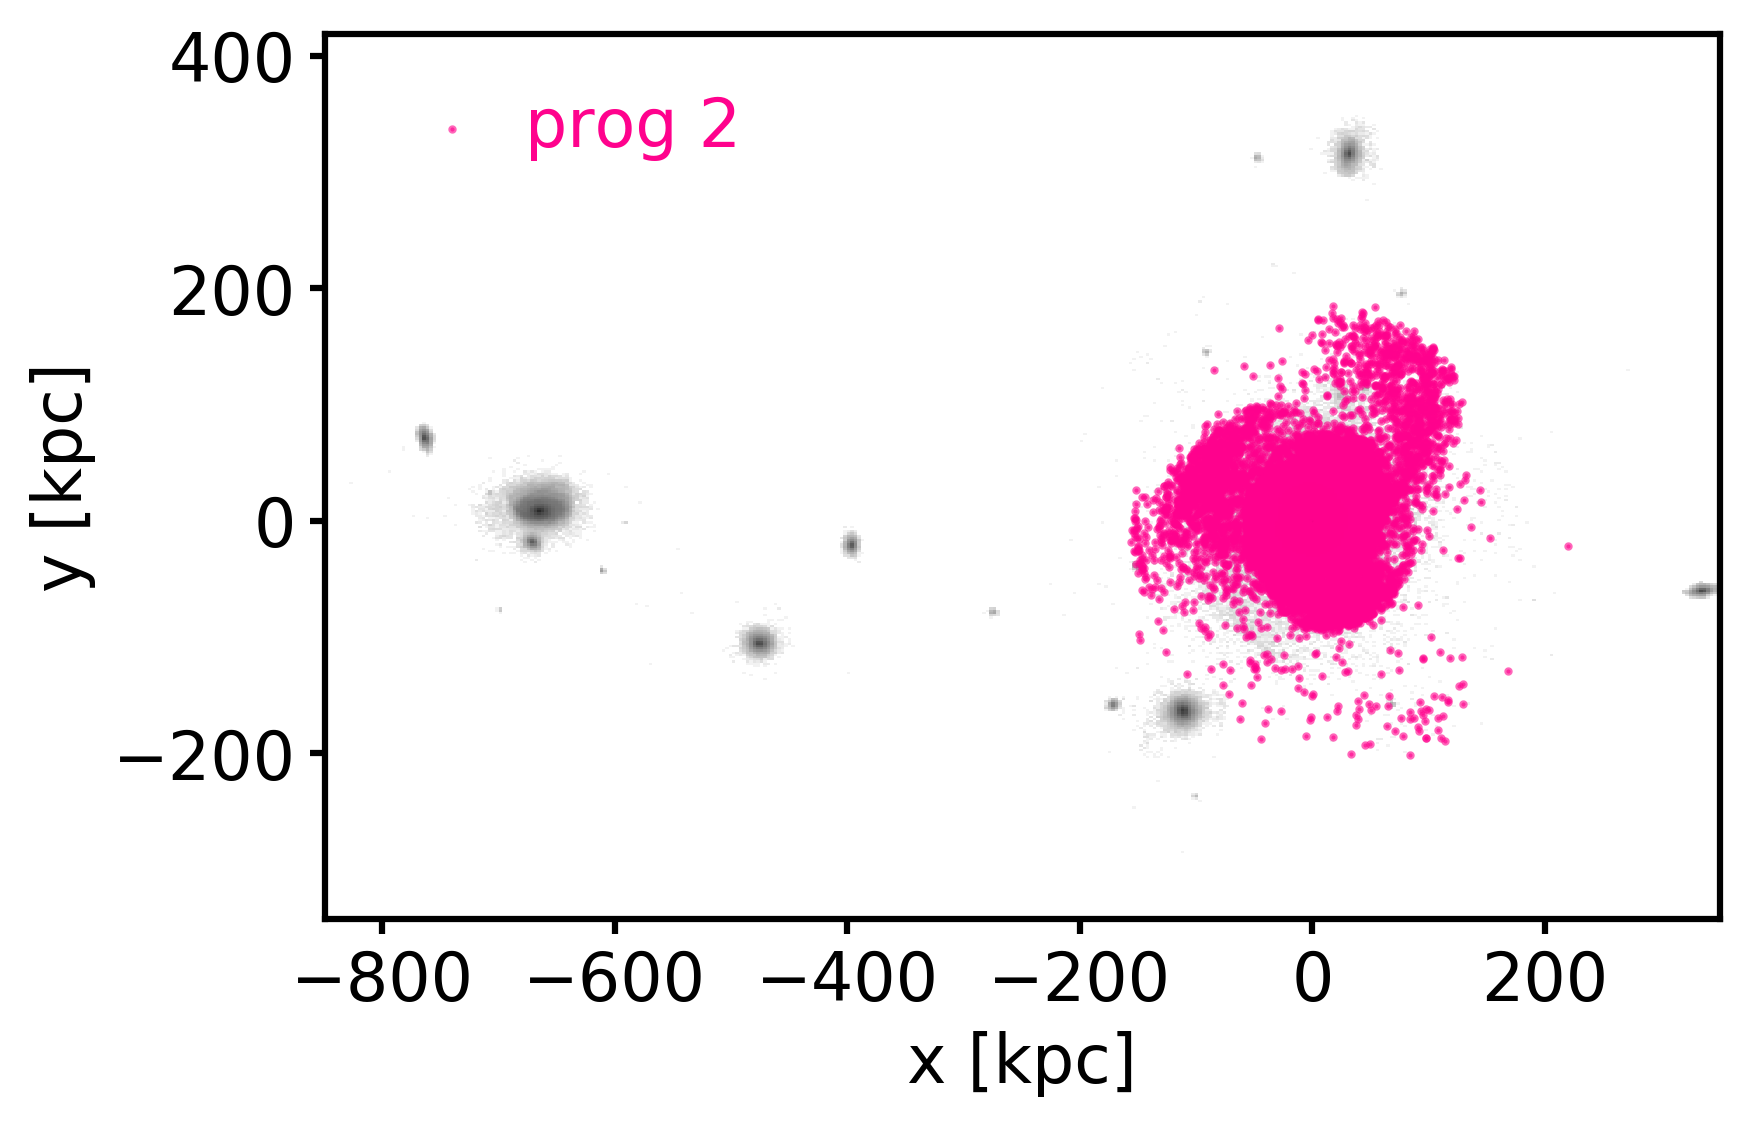
\includegraphics[width=\textwidth]{plots/Dynamics/dist/xy_dist_wodisk_GCs_prog_2_snap_127.png}
    	\label{fig:prog2_xy}
    \end{subfigure}
    ~ %add desired spacing between images, e. g. ~, \quad, \qquad, \hfill etc. 
    %(or a blank line to force the subfigure onto a new line)
    \begin{subfigure}[c]{0.48\textwidth}
        \centering
    	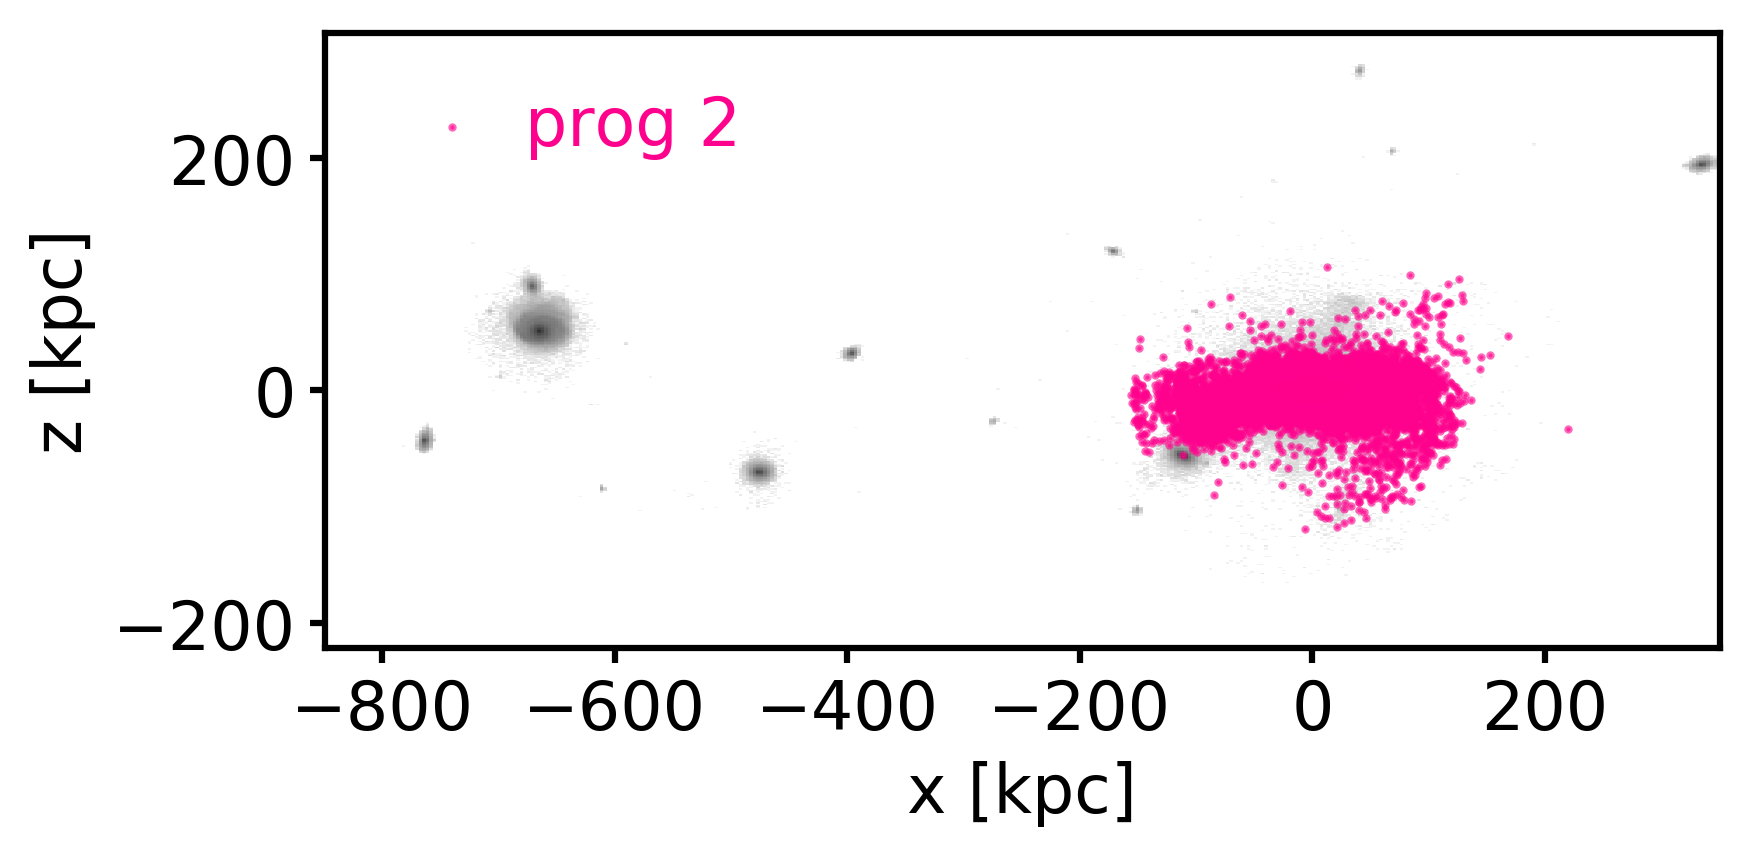
\includegraphics[width=\textwidth]{plots/Dynamics/dist/xz_dist_wodisk_GCs_prog_2_snap_127.png}
	    \label{fig:prog2_xz}
    \end{subfigure}
    
    \begin{subfigure}[c]{0.48\textwidth}
    \centering
    	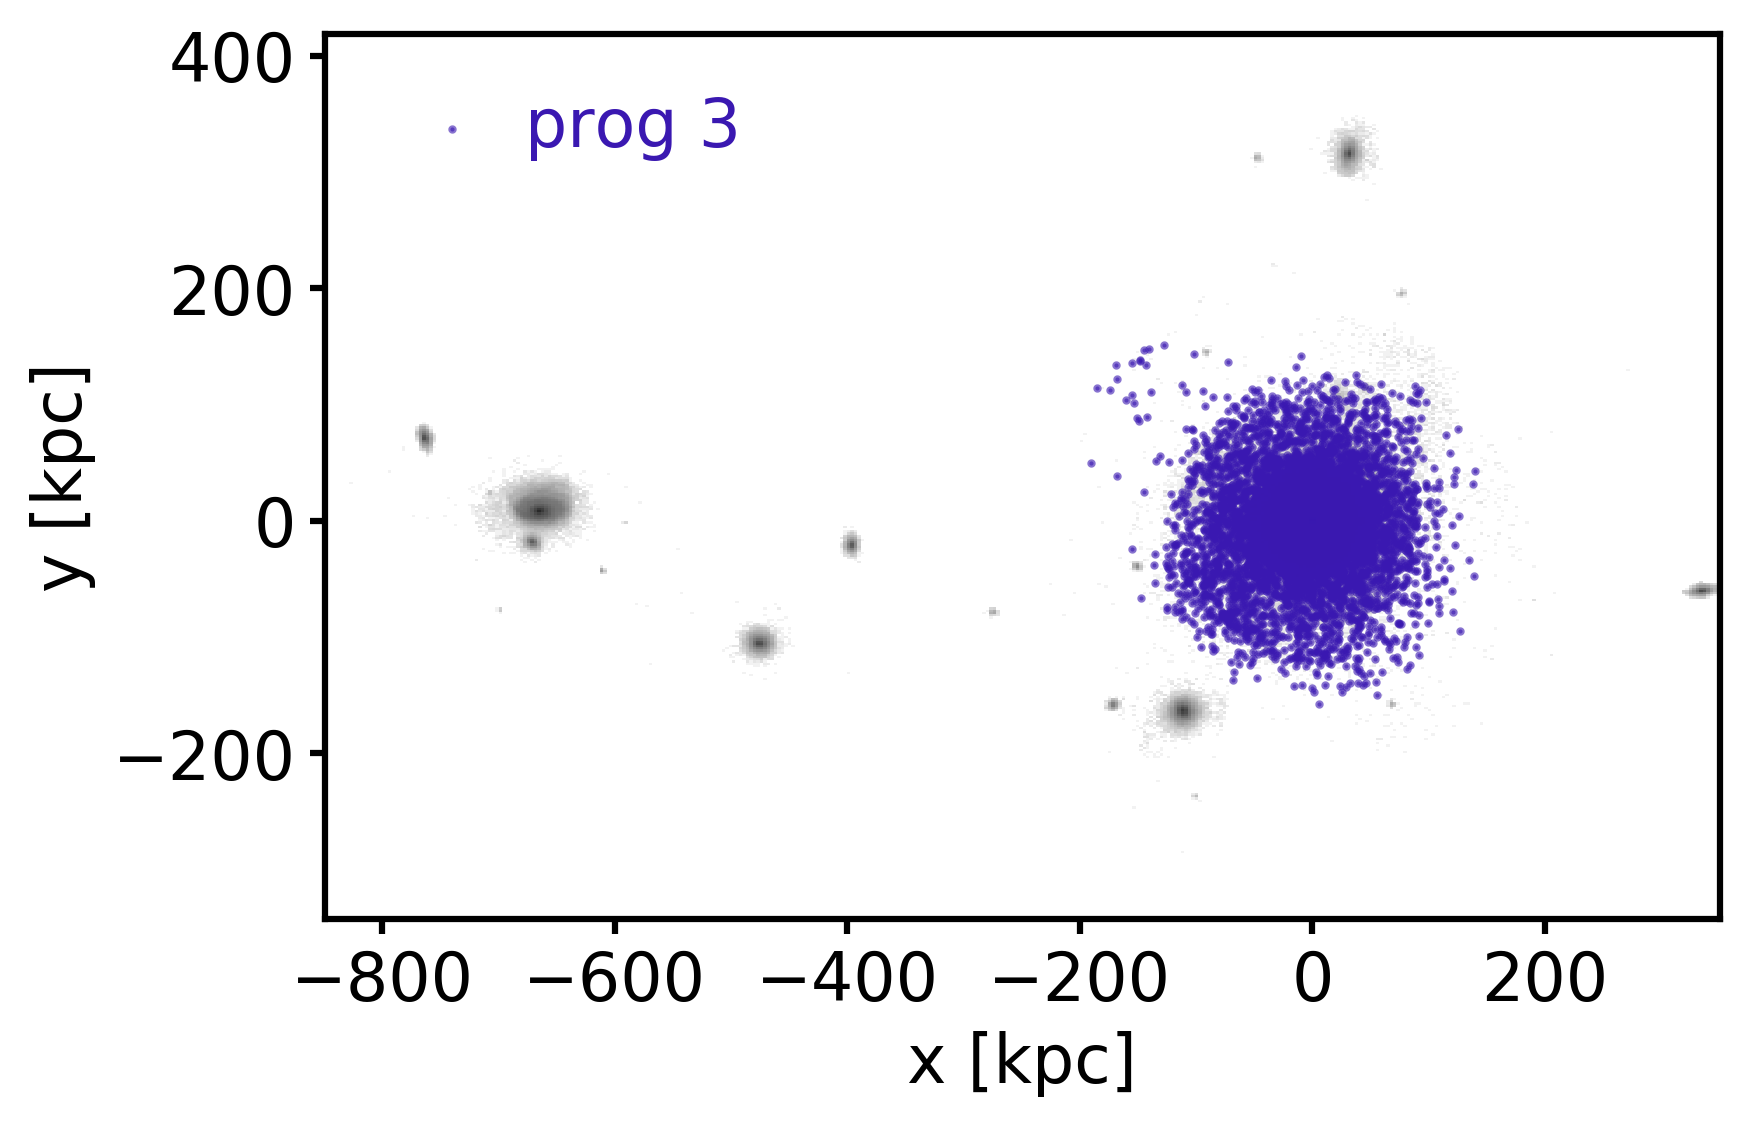
\includegraphics[width=\textwidth]{plots/Dynamics/dist/xy_dist_wodisk_GCs_prog_3_snap_127.png}
    	\label{fig:prog3_xy}
    \end{subfigure}
    ~ %add desired spacing between images, e. g. ~, \quad, \qquad, \hfill etc. 
    %(or a blank line to force the subfigure onto a new line)
    \begin{subfigure}[c]{0.48\textwidth}
        \centering
    	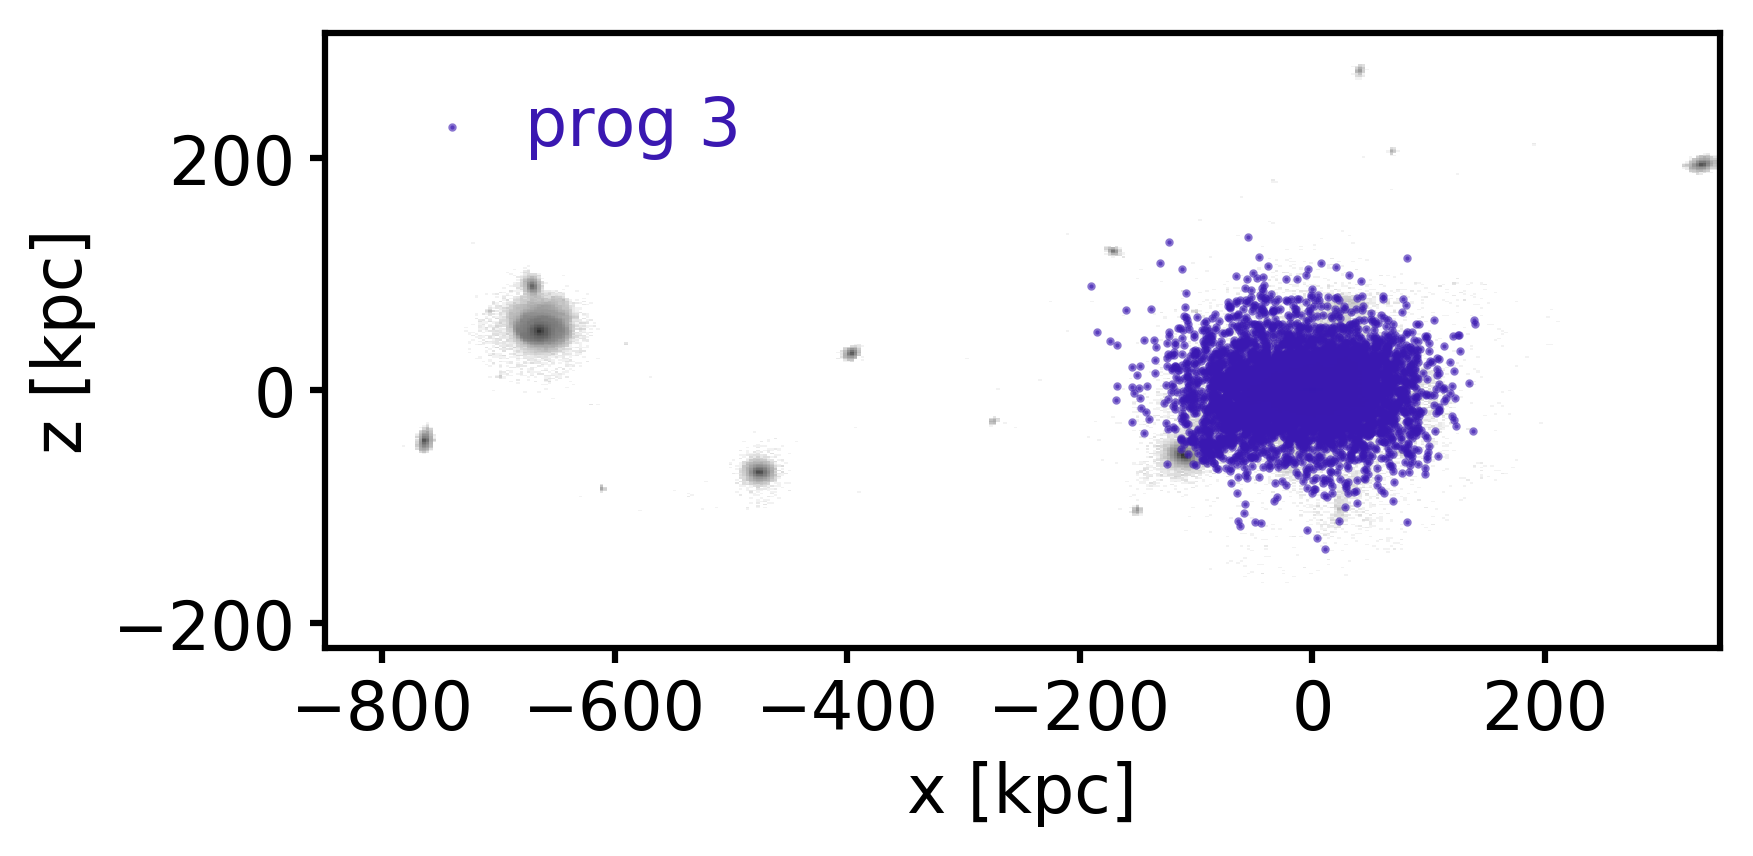
\includegraphics[width=\textwidth]{plots/Dynamics/dist/xz_dist_wodisk_GCs_prog_3_snap_127.png}
	    \label{fig:prog3_xz}
    \end{subfigure}
    
    \begin{subfigure}[c]{0.48\textwidth}
    \centering
    	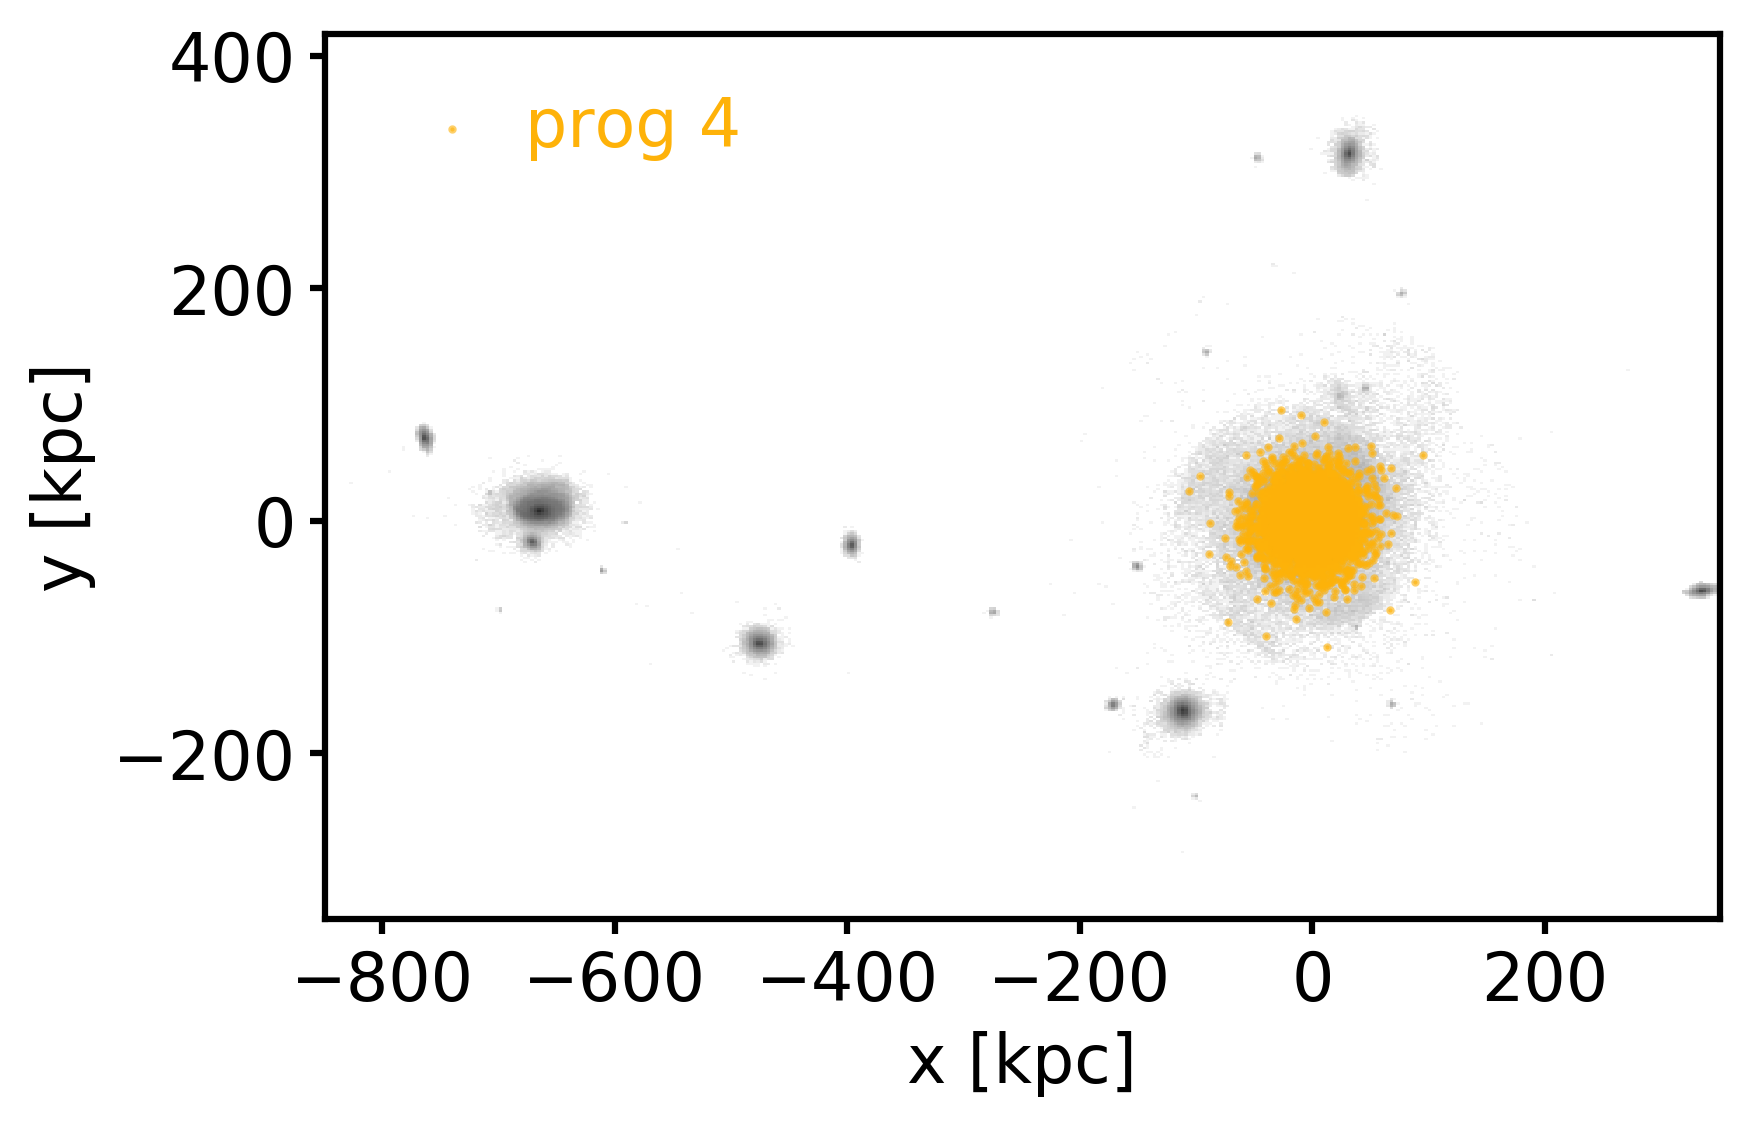
\includegraphics[width=\textwidth]{plots/Dynamics/dist/xy_dist_wodisk_GCs_prog_4_snap_127.png}
    	\label{fig:prog4_xy}
    \end{subfigure}
    ~ %add desired spacing between images, e. g. ~, \quad, \qquad, \hfill etc. 
    %(or a blank line to force the subfigure onto a new line)
    \begin{subfigure}[c]{0.48\textwidth}
        \centering
    	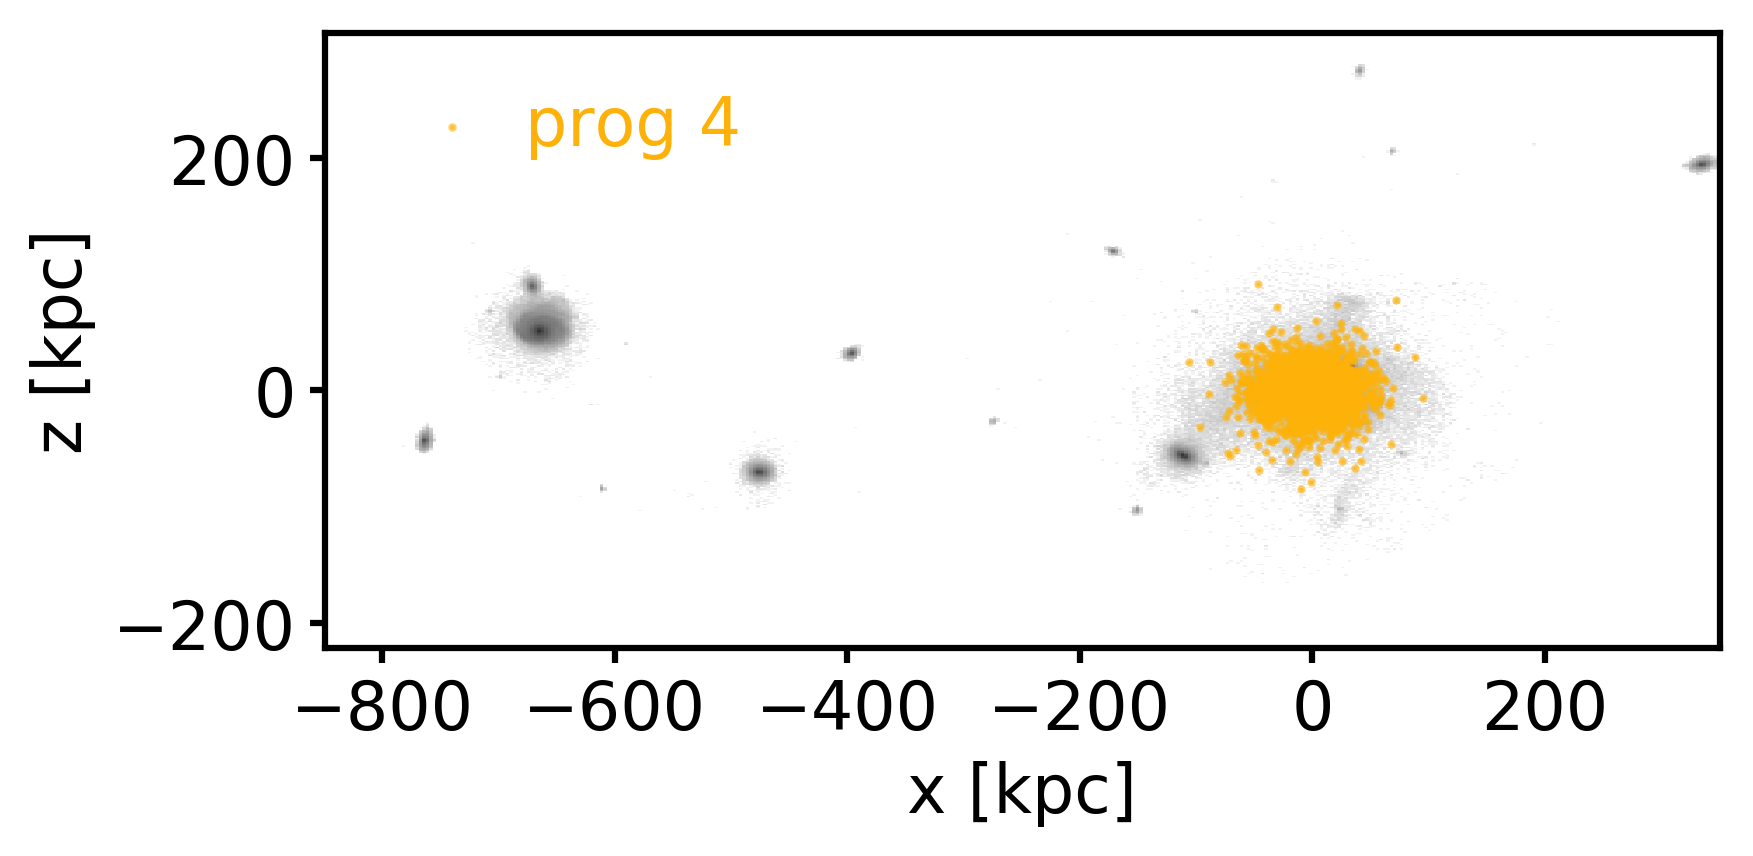
\includegraphics[width=\textwidth]{plots/Dynamics/dist/xz_dist_wodisk_GCs_prog_4_snap_127.png}
	    \label{fig:prog4_xz}
    \end{subfigure}
    \caption{Remnants of the three biggest \ac{DG} mergers which were not destroyed by the disk. The left panels show the x-y number distribution, the right panels the x-z distribution. In grey, the main galaxy and its satellites are plotted (as in Figure \ref{fig:Stars_AU24}). \textit{Upper panels}: The remnants of the most recent merger are plotted in pink. \textit{Middle panel}: The blue points are remnants of the second biggest merger. \textit{Lower panel}: The yellow points are remnants of the third biggest merger which is the most long ago of these three. These remnants will be considered the \ac{GC} populations of each merger event.}\label{fig:progenitors_distribution}
\end{figure}
The positions of the remnants of these three merger events are shown in Figure \ref{fig:progenitors_distribution}. Prog3 and prog4 are totally dispersed in the galaxy while prog2 still shows some merging features such as broad streams, especially visible face-on. Prog2 has nearly a factor of 100 more remaining \acp{GC} than the other two progenitors. This is due to the short time it is in the main galaxy and therefore could these \acp{GC} are neither as much dissolved as the others nor as much disrupted by the disk. Since these three mergers are so different at redshift 0, it is interesting to test their behaviour in action space, where dynamical features are expected to be visible longer. 

\subsection{Globular clusters in action space}\label{subsec:GCs_action_space}
Now, we look at the \ac{GC} distribution in action space. Our assumption is that in the "true" potential, \acp{GC} are very clumped since they should retain dynamical memory from their former \ac{DG} and therefore their \ac{DF} should be a delta function. In section \ref{subsubsec:GCs_actions_right_pot}, we will look at the distribution in the fitted potential at redshift 0. In section \ref{subsubsec:GCs_actions_varying_pot}, we evaluate actions in varying potentials to test our assumption of \acp{GC} being most clumped in action space in the "true" potential. 

\subsubsection{Best fit potential}\label{subsubsec:GCs_actions_right_pot}

\begin{figure}[htbp]
\captionsetup{format=plain}
    \centering
    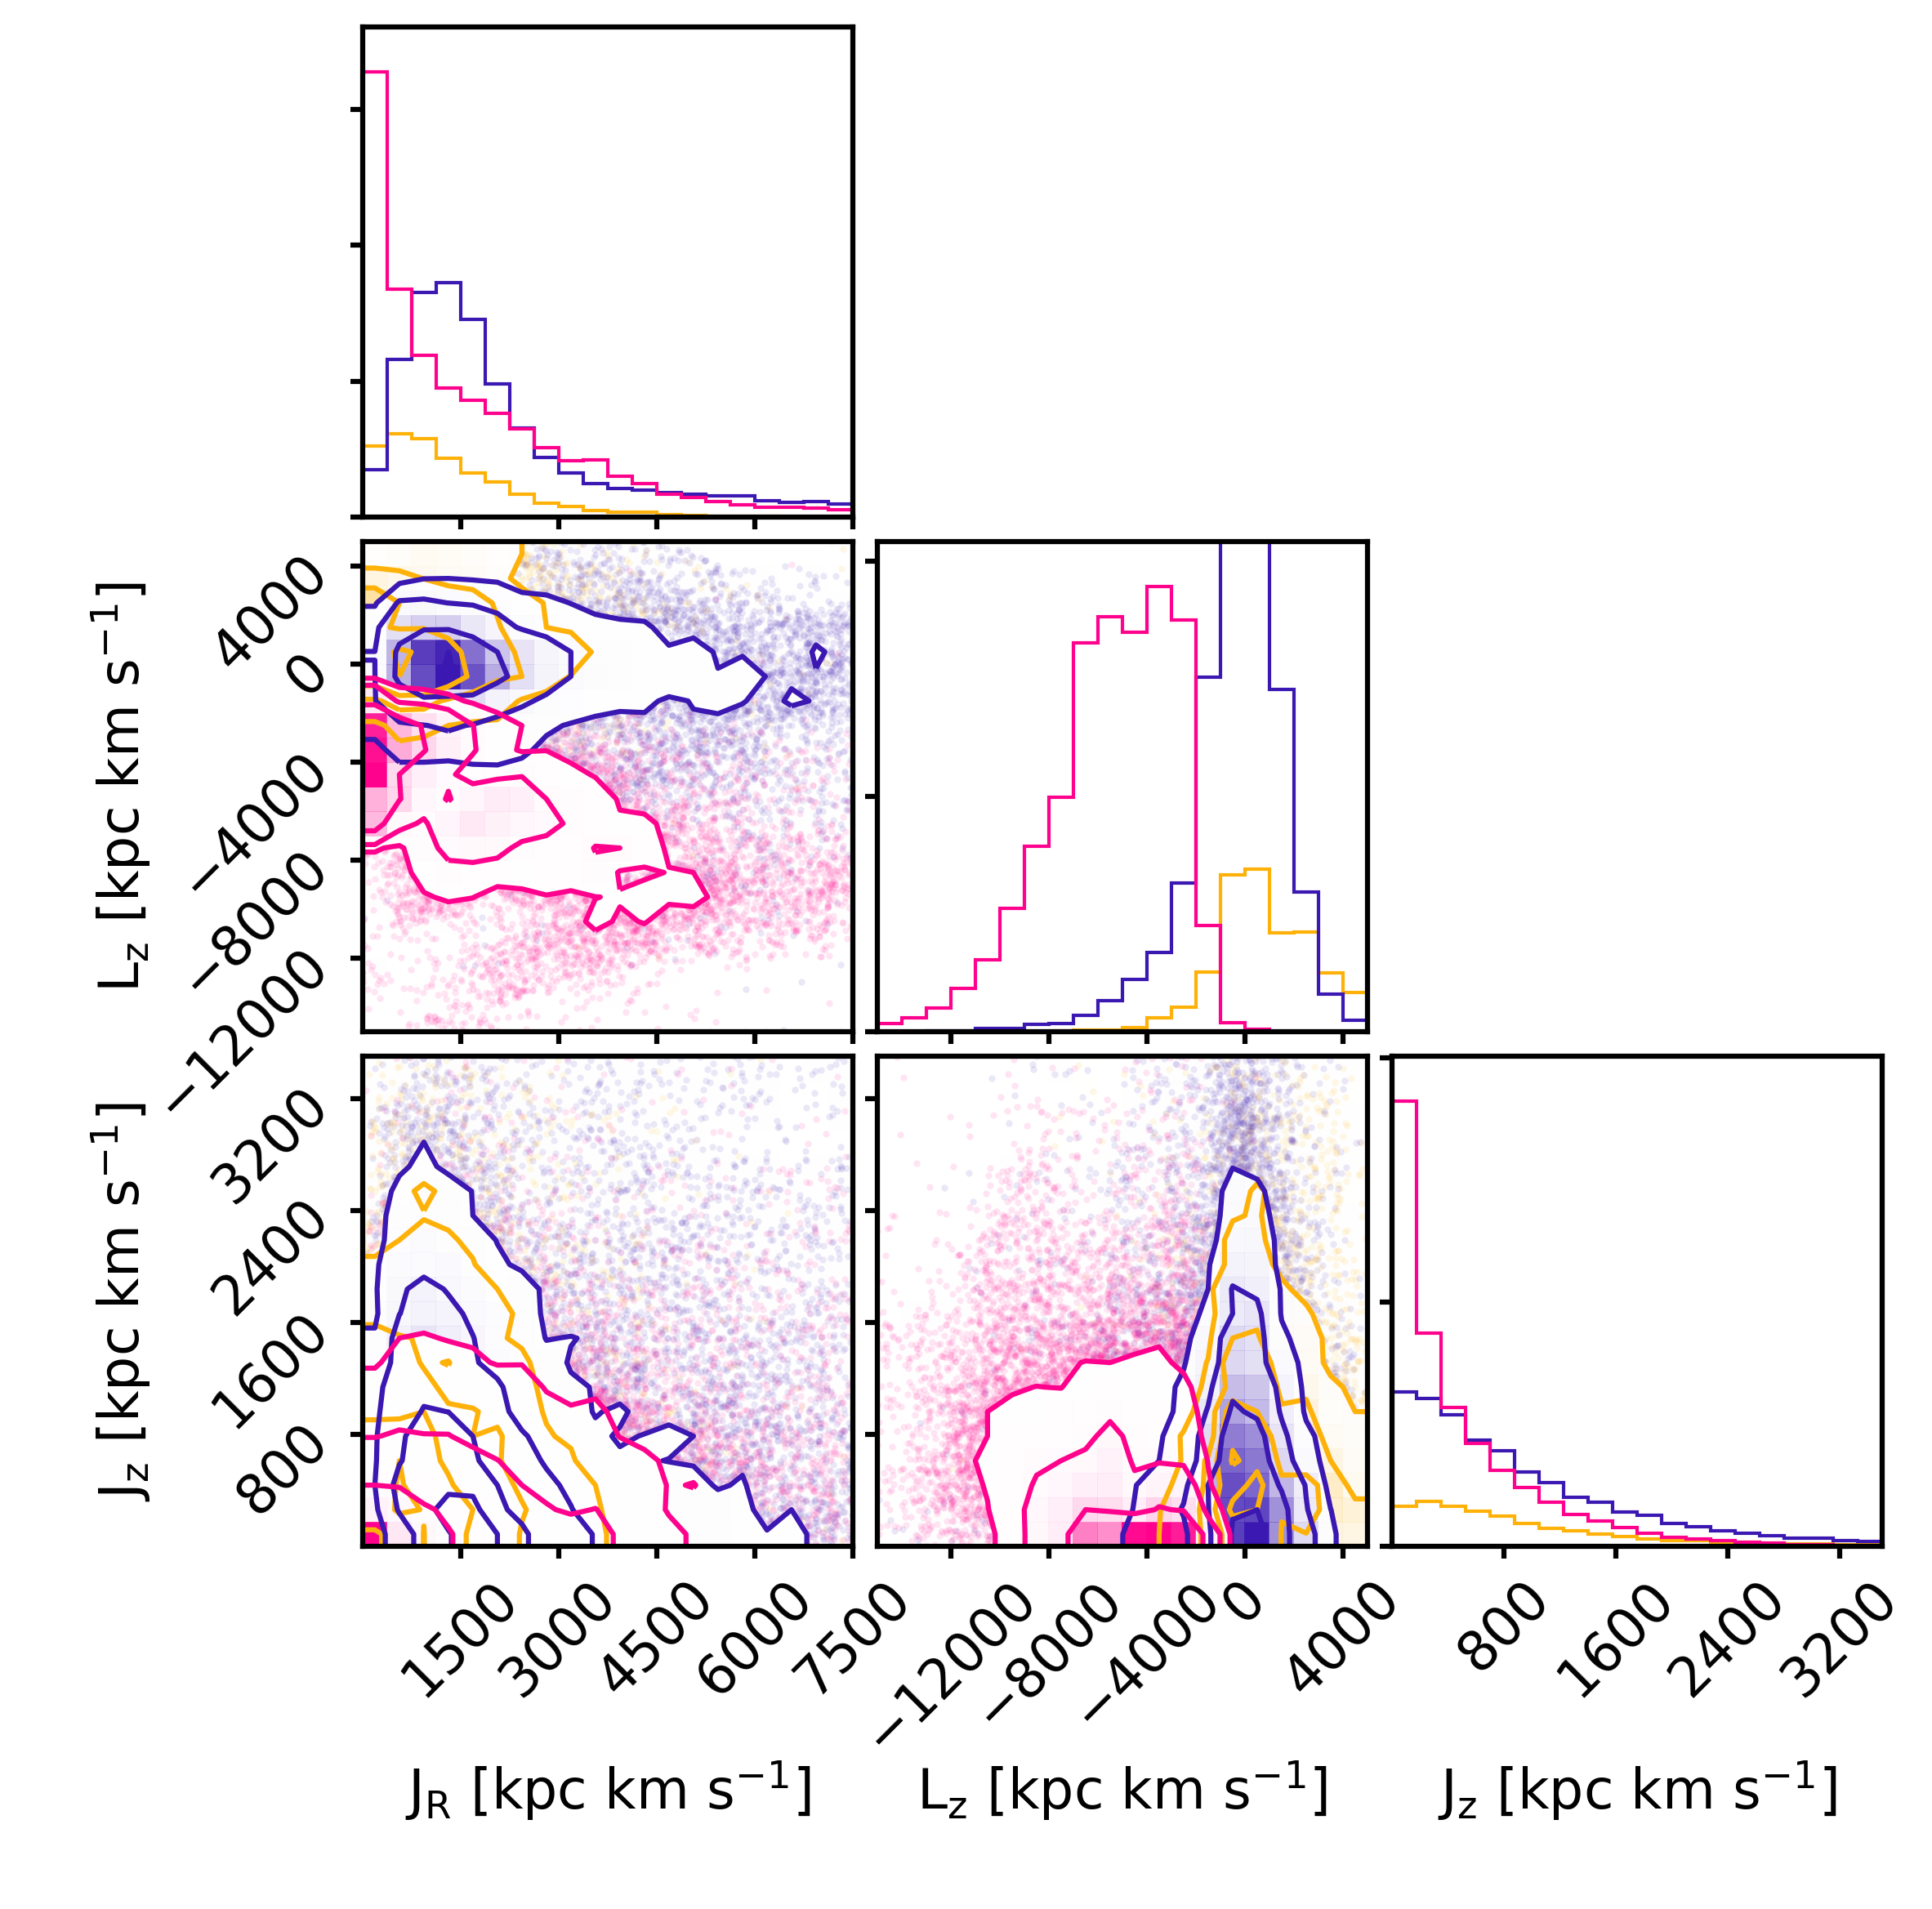
\includegraphics[width=1.0\textwidth]{plots/Dynamics/prog234_GCwodisk_actions_snap_127.png}
    \caption{Selected \acp{GC} from three different \acp{DG} in action space. The diagonal elements show histograms of each action and the other panels show 2D histograms of each action pair. In pink/blue/yellow, we see the action distribution of the remnants of prog2/prog3/prog4. Since we have many more particles from prog2, the histograms in the diagonal elements are dominated by their distribution. In the correlation panels, we can clearly distinguish prog 2 and prog 4 while prog 3 is very dispersed and does not have an identifiable center in any action. Even though the merger of prog4 happened the longest ago, it is still very clumped in all combinations, with the most clumpiness in $J_R - L_z$. The distribution of prog2 is narrow in $L_z$ but very broad in $J_R - J_z$. prog2 is corotating with the disk but with a higher angular momentum than the disk has (\(\overline{L_z} = SI{-2235}{kpc.km.s^{-1}}\)). prog4 is clearly counter rotating.}
    \label{fig:act_all_merg_best_pot}
\end{figure}
We calculate the actions of the remnants of each progenitor in the best fit potential and plot them in Figure \ref{fig:act_all_merg_best_pot}. The remnants of the different merger events are best distinguishable in L$_\mathrm{Z}$. Prog2 is corotating with the disk but with higher angular momentum. Prog4 is counter rotating. Prog3 is more dispersed in L$_\mathrm{Z}$ but its mean is corotating with the disk as well. In the vertical action, the three remnant groups are not distinguishable and have means at \SI{1000-2000}{kpc.km.s^{-1}}. In J$_\mathrm{R}$, the groups are again distinguishable. 
\\The idea of this method is that in the right potential, these groups minimize their spread in action space. Prog4 is the most compact group, while especially prog3 is very dispersed. To quantify the compactness, we measure the standard deviation of each action. In the next Section, we compare the standard deviations of the radial and vertical actions of each group in different potentials to see, if we minimize them in the 'true' potential.

\subsubsection{Varying potentials}\label{subsubsec:GCs_actions_varying_pot}
To vary the potential in way it should affect the groups the most, we vary the \ac{DM} halo. We do this by keeping all best fit potential parameters constant and only vary the scale length $a_\mathrm{NFW}$. For the three groups in these potentials, we calculate the actions in the $z=0$ snapshot.
\begin{figure}[!ht]
\captionsetup{format=plain}
   \subfloat{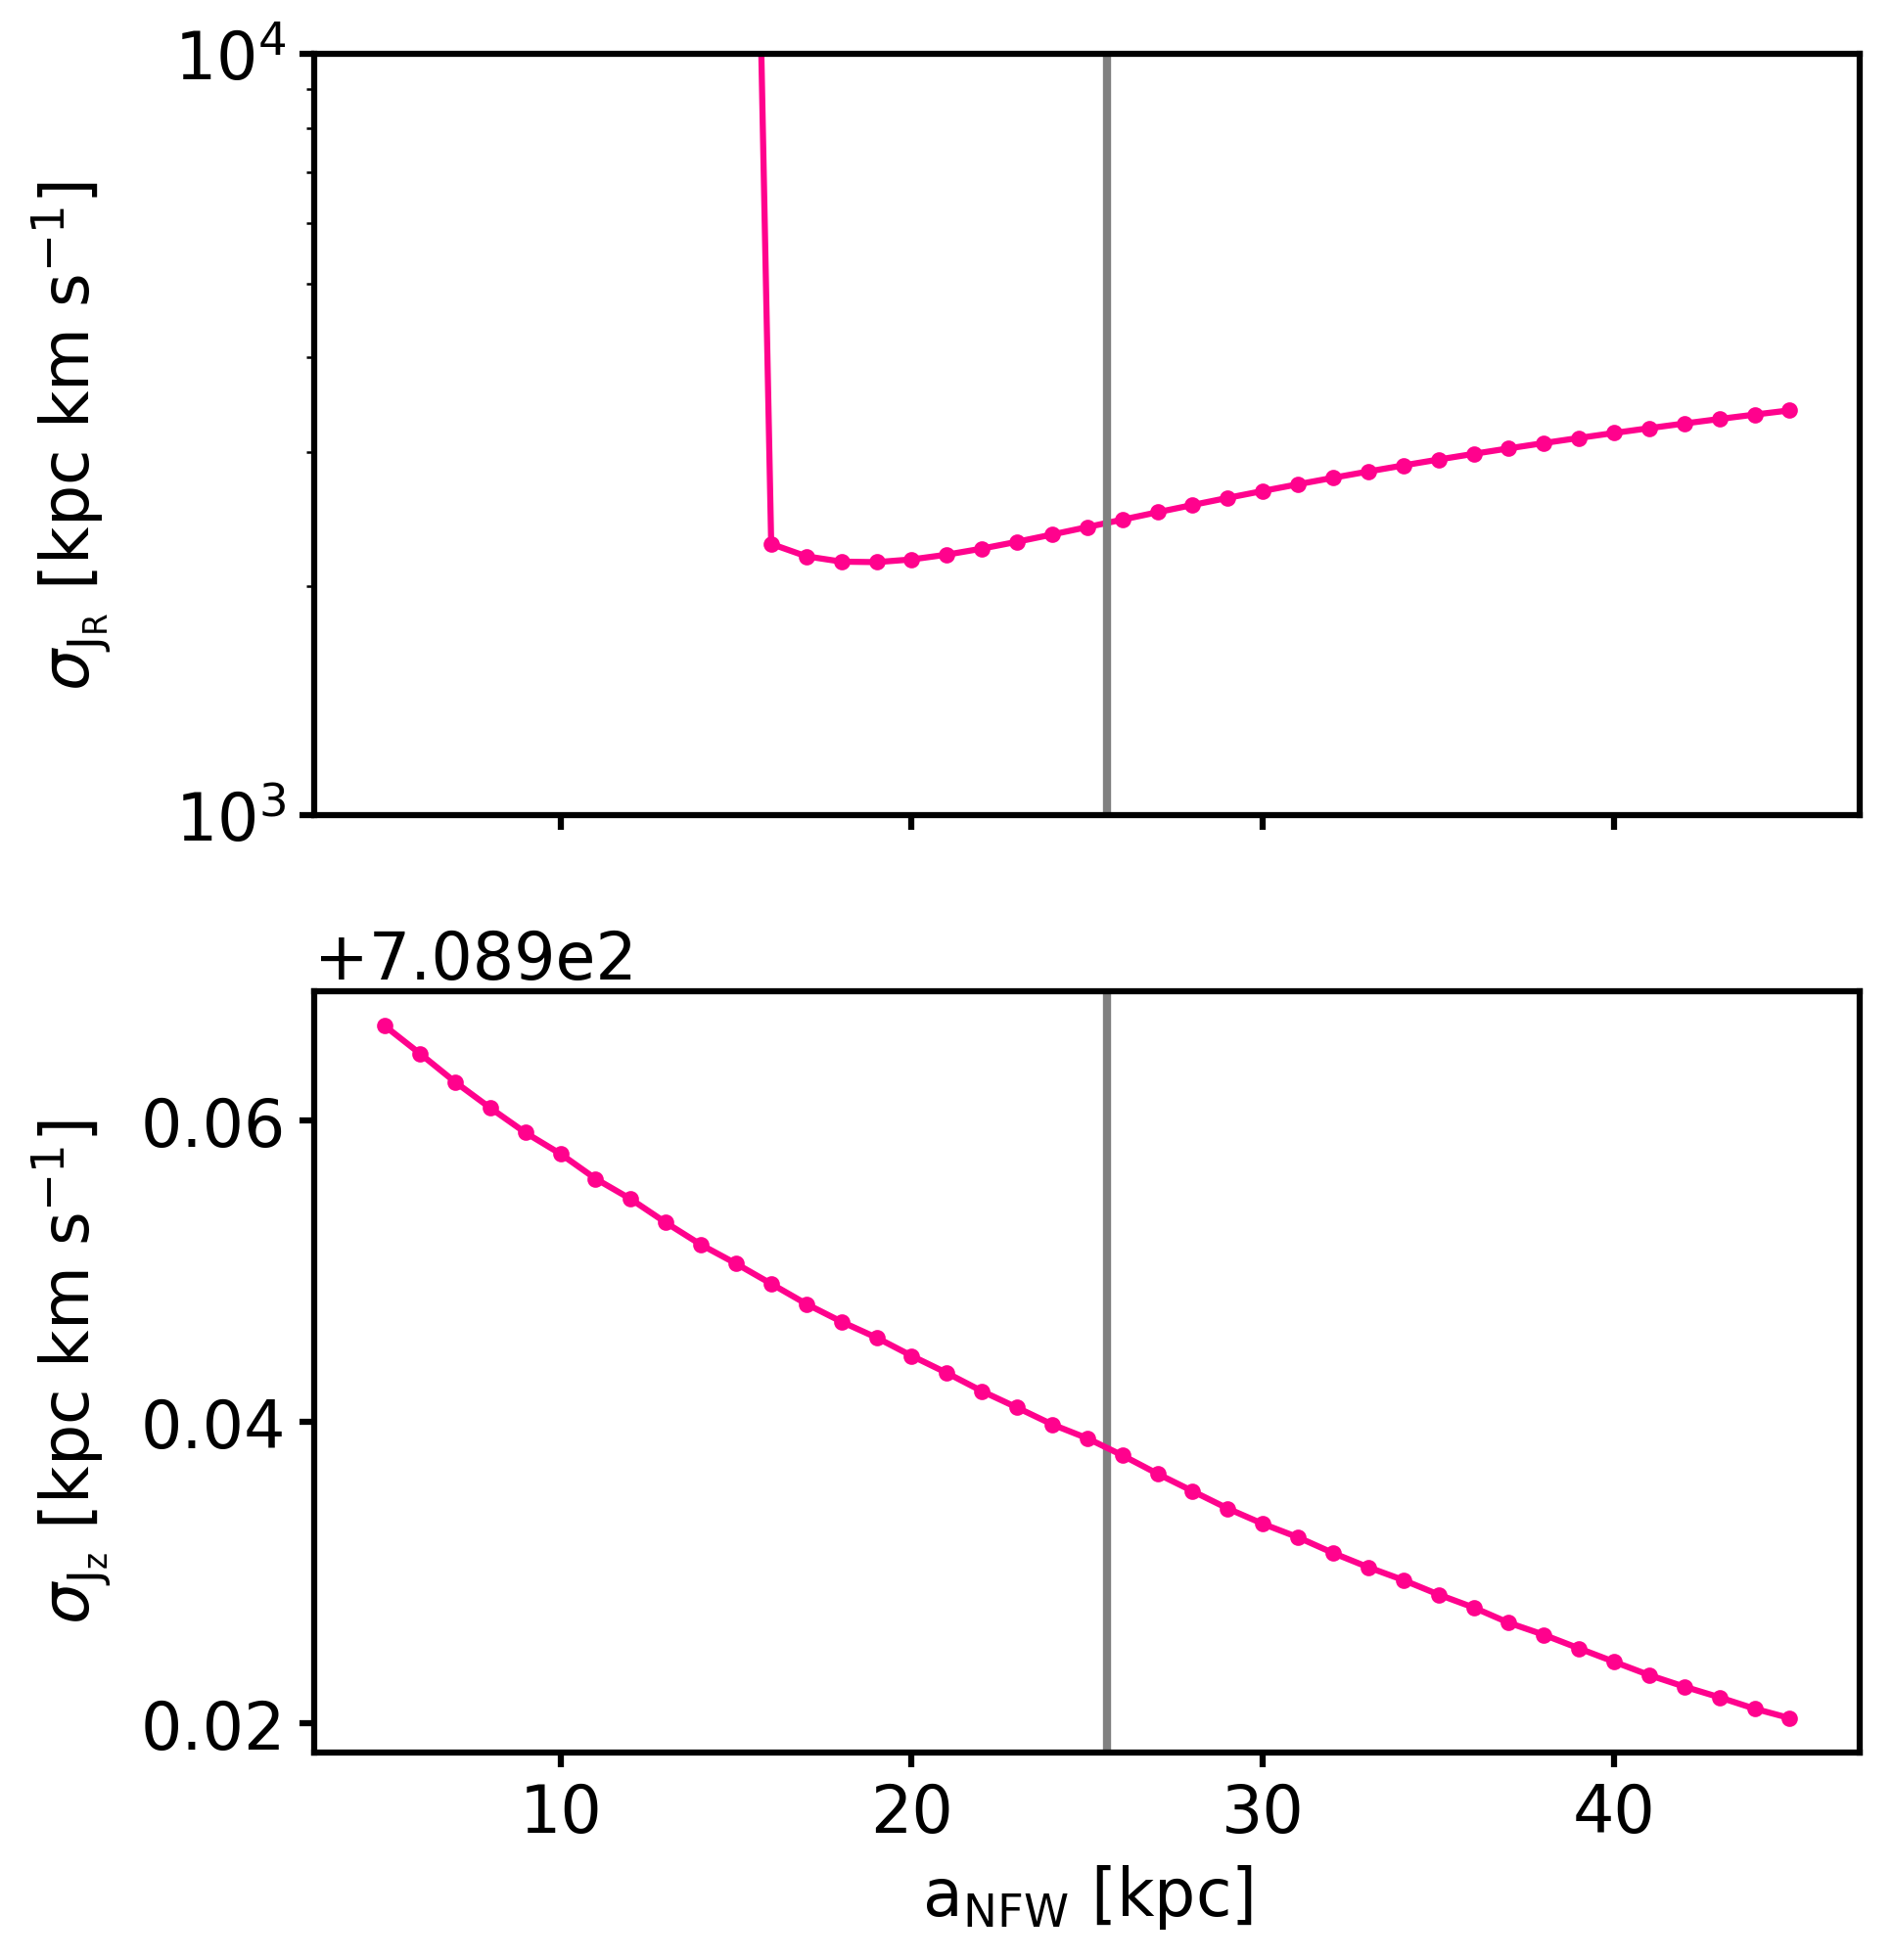
\includegraphics[width=0.48\textwidth]{plots/Dynamics/prog2/a_NFW_diagnostic_plot_std_prog2_all.png}}\hfill%
   \subfloat{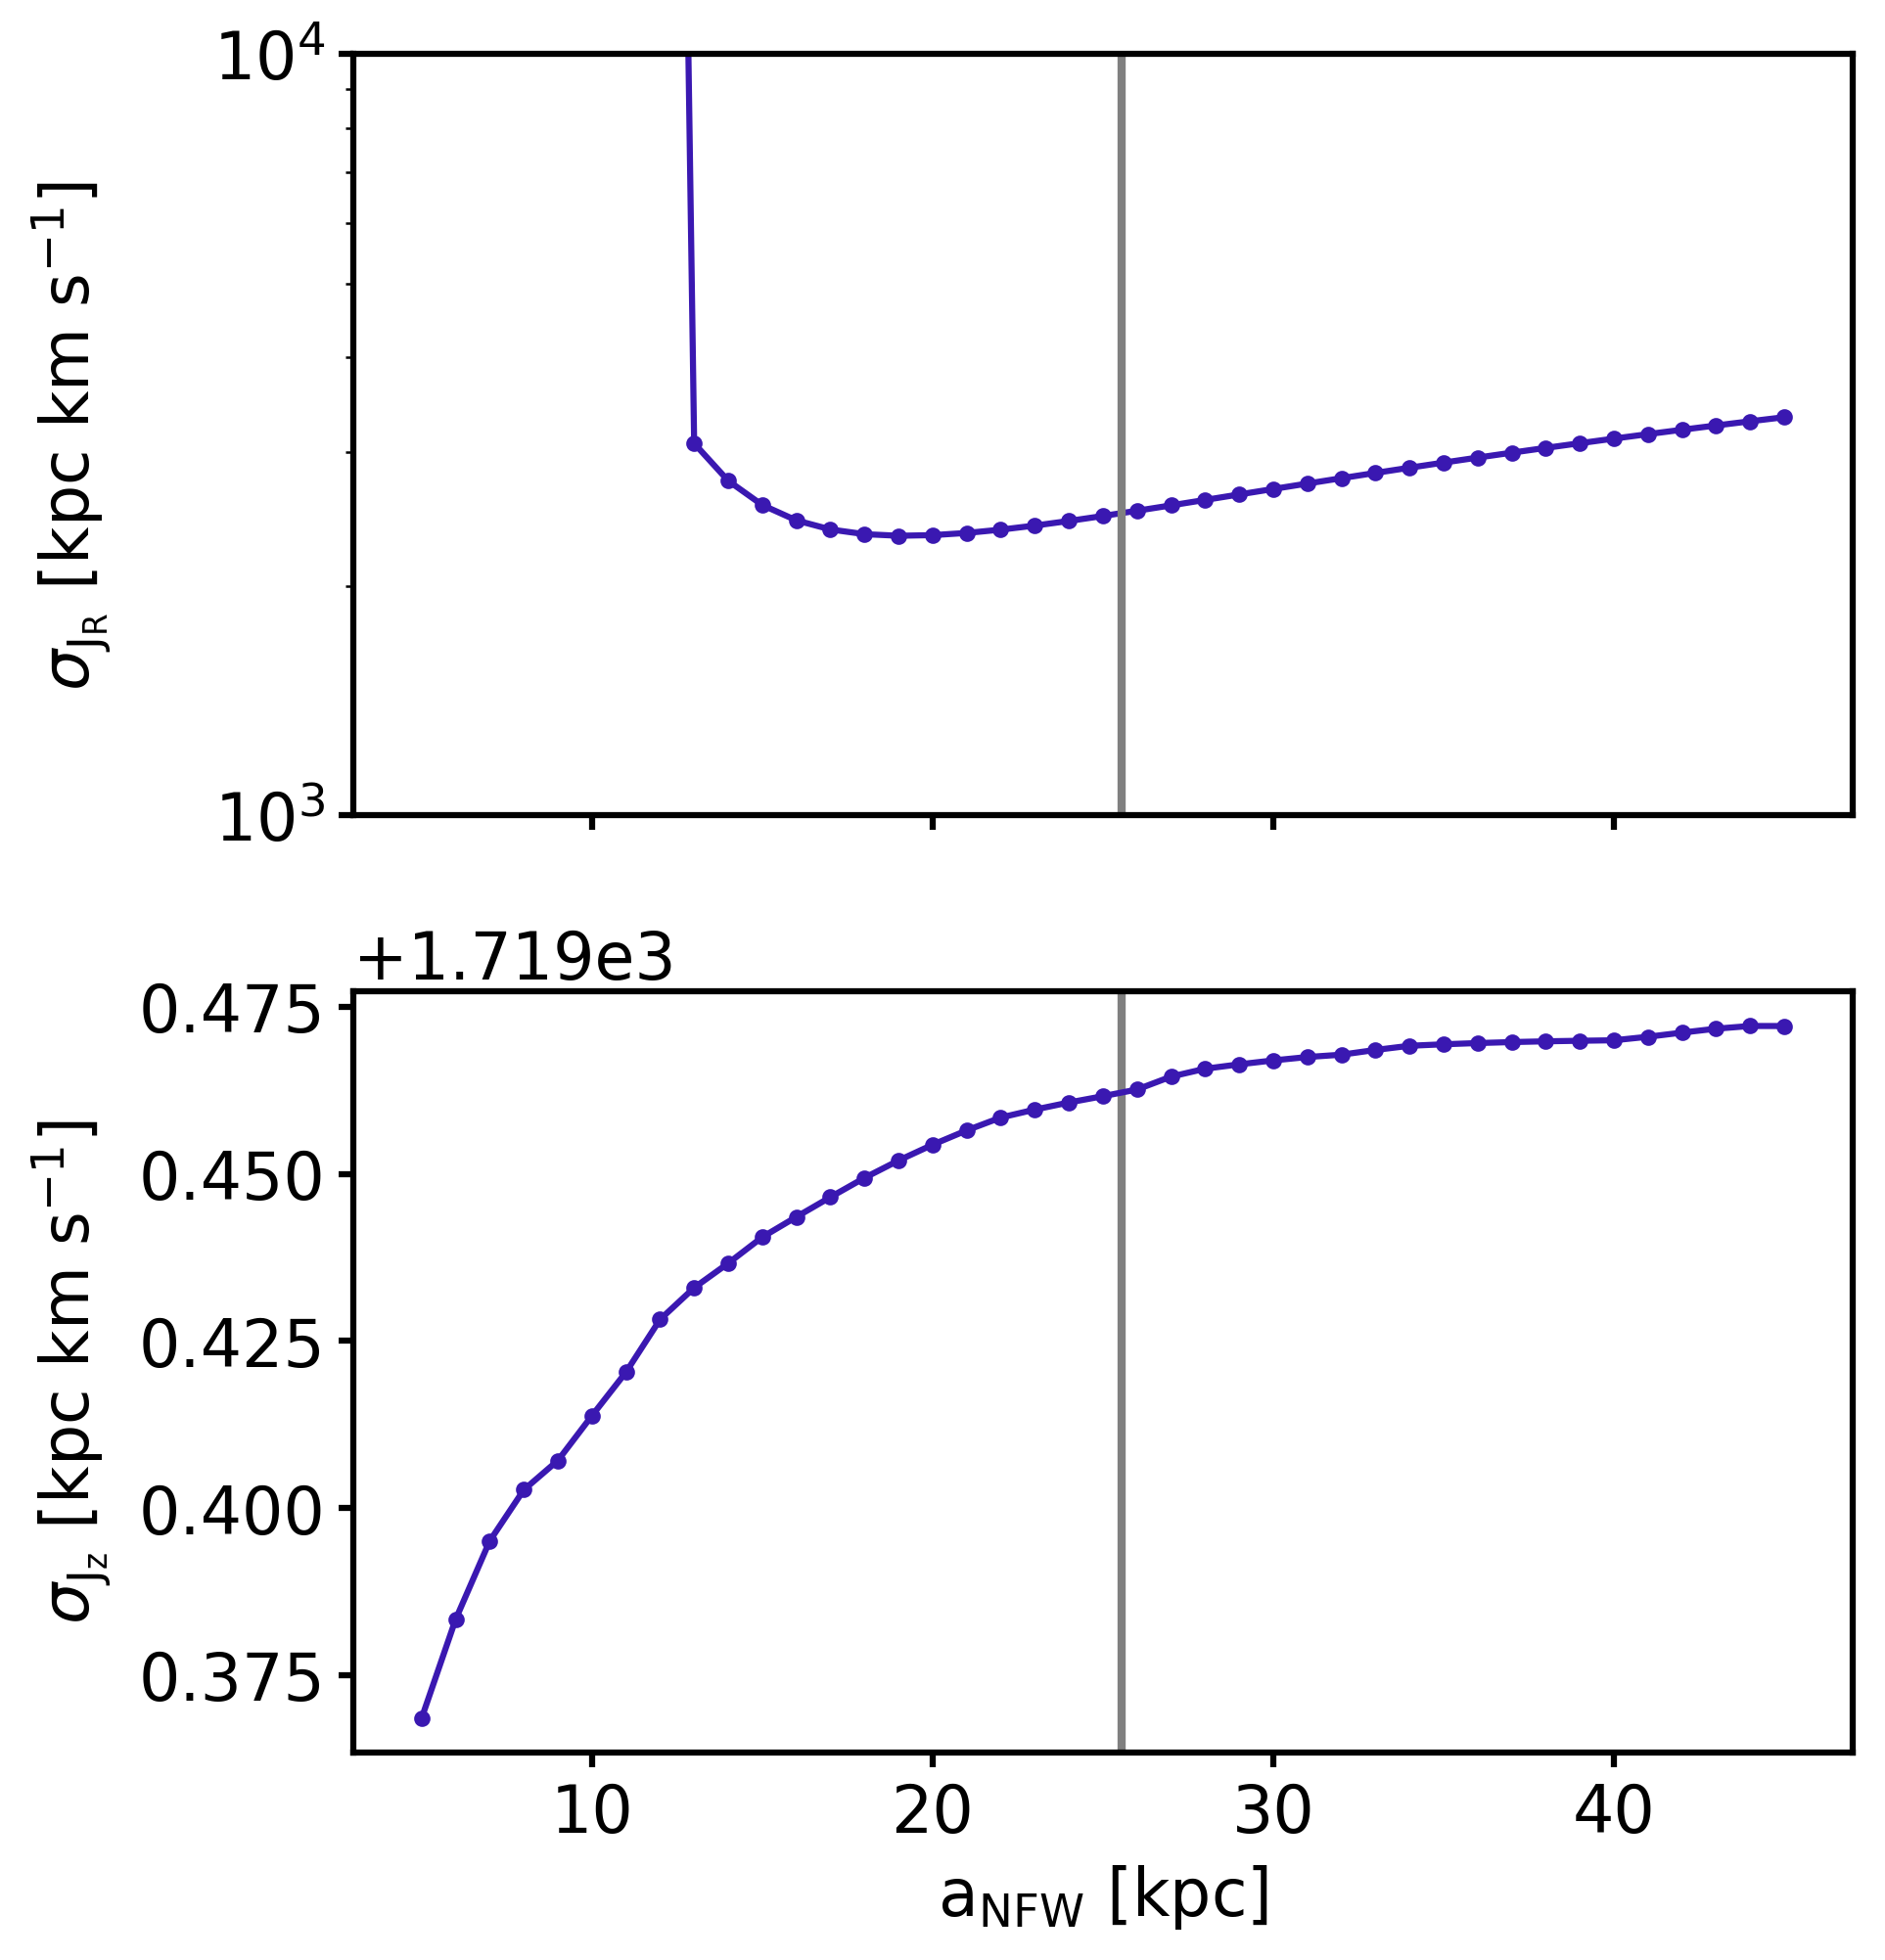
\includegraphics[width=0.48\textwidth]{plots/Dynamics/prog3/a_NFW_diagnostic_plot_std_prog3_all.png}}\vspace*{0.5cm}\par
   \subfloat{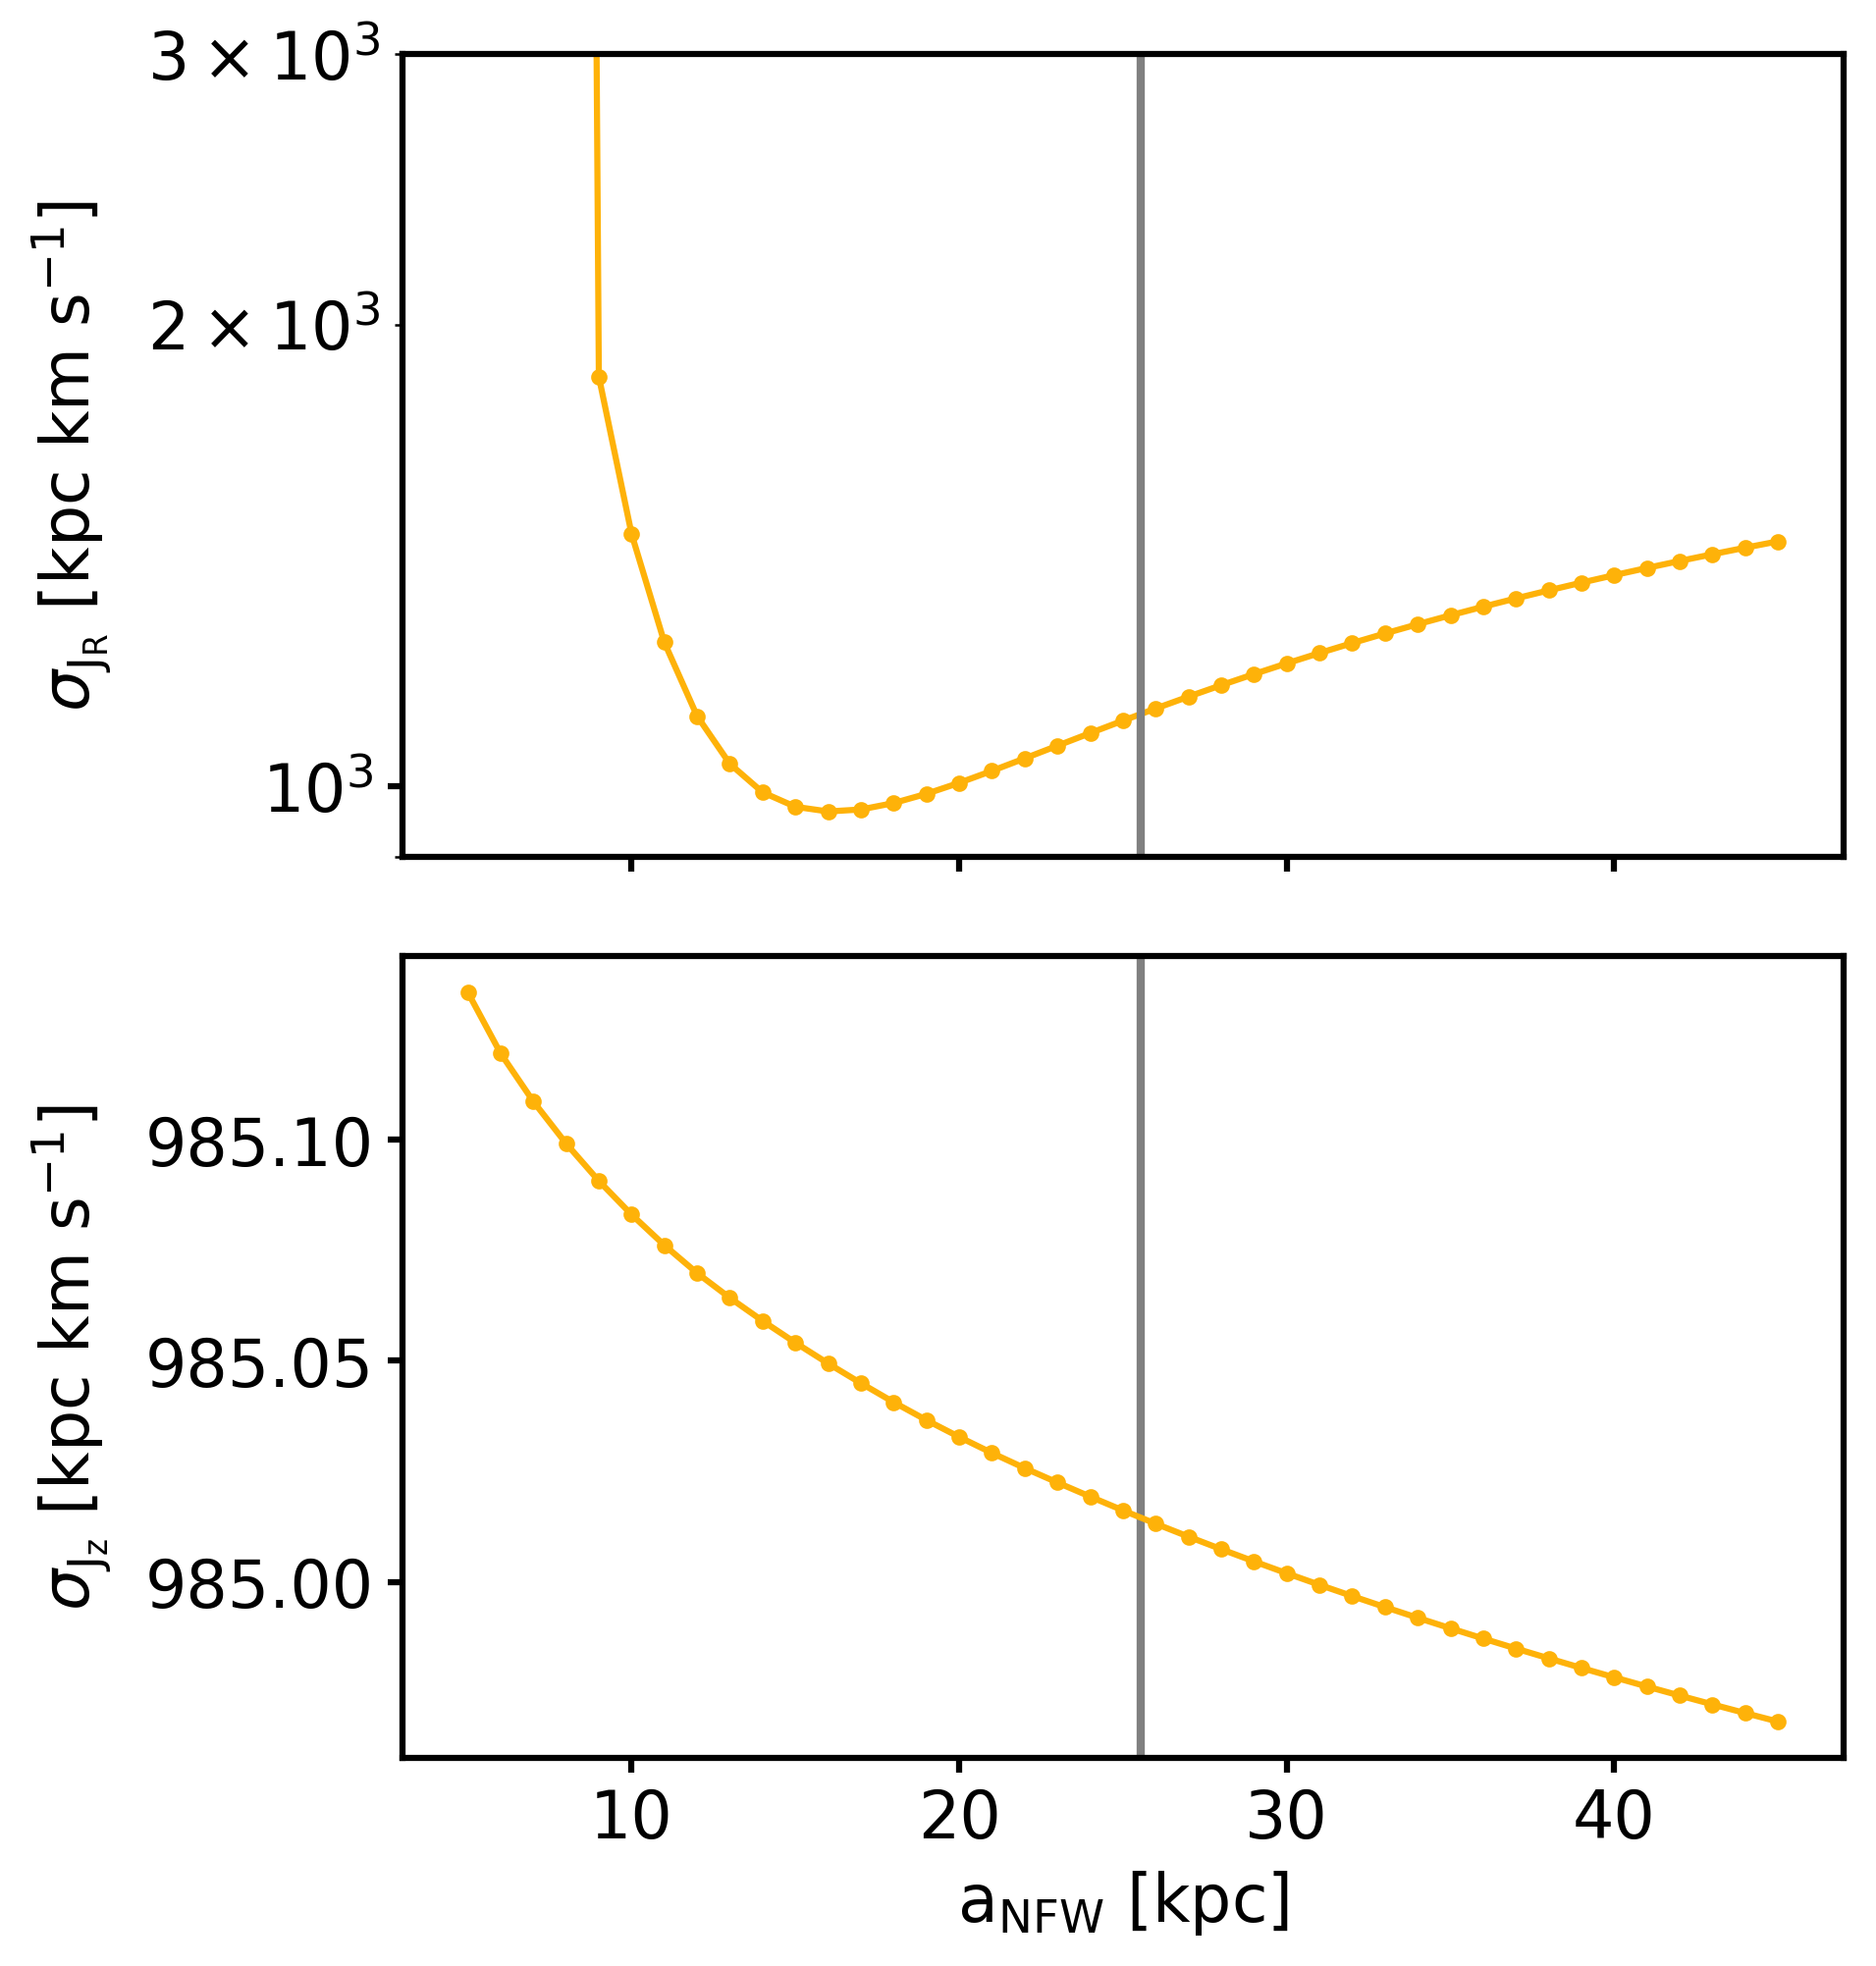
\includegraphics[width=0.48\textwidth]{plots/Dynamics/prog4/a_NFW_diagnostic_plot_std_prog4_all.png}}\hfill%
   \parbox[b][.3\textheight]{.48\textwidth}%
     {\vskip-\abovecaptionskip\RawCaption{\caption{Standard deviations of the radial and vertical actions of all three mergers (prog2-pink / prog3-blue / prog4-yellow) in potentials with varying scale length of the \ac{DM} halo and all other parameters kept on their best fit value. We would expect the standard deviation to be mimized at the best fit potential which is indicated with the vertical grey line. We see that the radial action would prefer a lower scale length (at \SI{17}{kpc}) while two of the three vertical actions would prefer higher scale lengths. The differences in $\sigma_{J_z}$ are much smaller than the one in $\sigma_{J_R}$. \textcolor{red}{update with new selected GCs coming}}\vfill\label{fig:a_NFW_diagnostic_plots}}}
\end{figure}
In Figure \ref{fig:a_NFW_diagnostic_plots}, we see how the standard deviations of the radial and vertical actions evolve in the different potentials. For all three \acp{GC} groups we see that in the radial action they would prefer a smaller scale length of the halo potential. The changes in vertical action are very small but two of three groups would prefer a larger scale length. 
\\\\This leads us to the conclusion that in the 'true' potential, the \acp{DF} of accreted \acp{GC} of one \ac{DG} are not $\delta$-functions but more complex. We cannot constrain an analytic axisymmetric gravitational potential by only minimizing the spread of these \acp{GC} in action space.

\subsection{Time evolution of actions}\label{subsec:time_evo_actions}
We evaluate the time evolution of the orbits of the accreted \acp{GC} to investigate how the actions evolved and to see if there was a point - probably shortly after their mergers - where the \acp{GC} were more clumped in action space and the \ac{DF} could have been a $\delta$-function. If that would be true, we could at least determine the potential of galaxies which are in a state shortly after a minor merger. We calculate the actions of the selected particles in the best fit potential in each snapshot.  

\subsubsection{Best fit potential}\label{subsubsec:GCs_action_time_right_pot}
With the method described in Section \ref{subsec:best_fit_pot} we fit an analytic axisymmetric potential to each snapshot individually. We trace back the \acp{GC} we considered as merged and calculate their actions in each snapshot for both after and before the merger. 
\begin{figure}[htbp]
\captionsetup{format=plain}
    \centering
	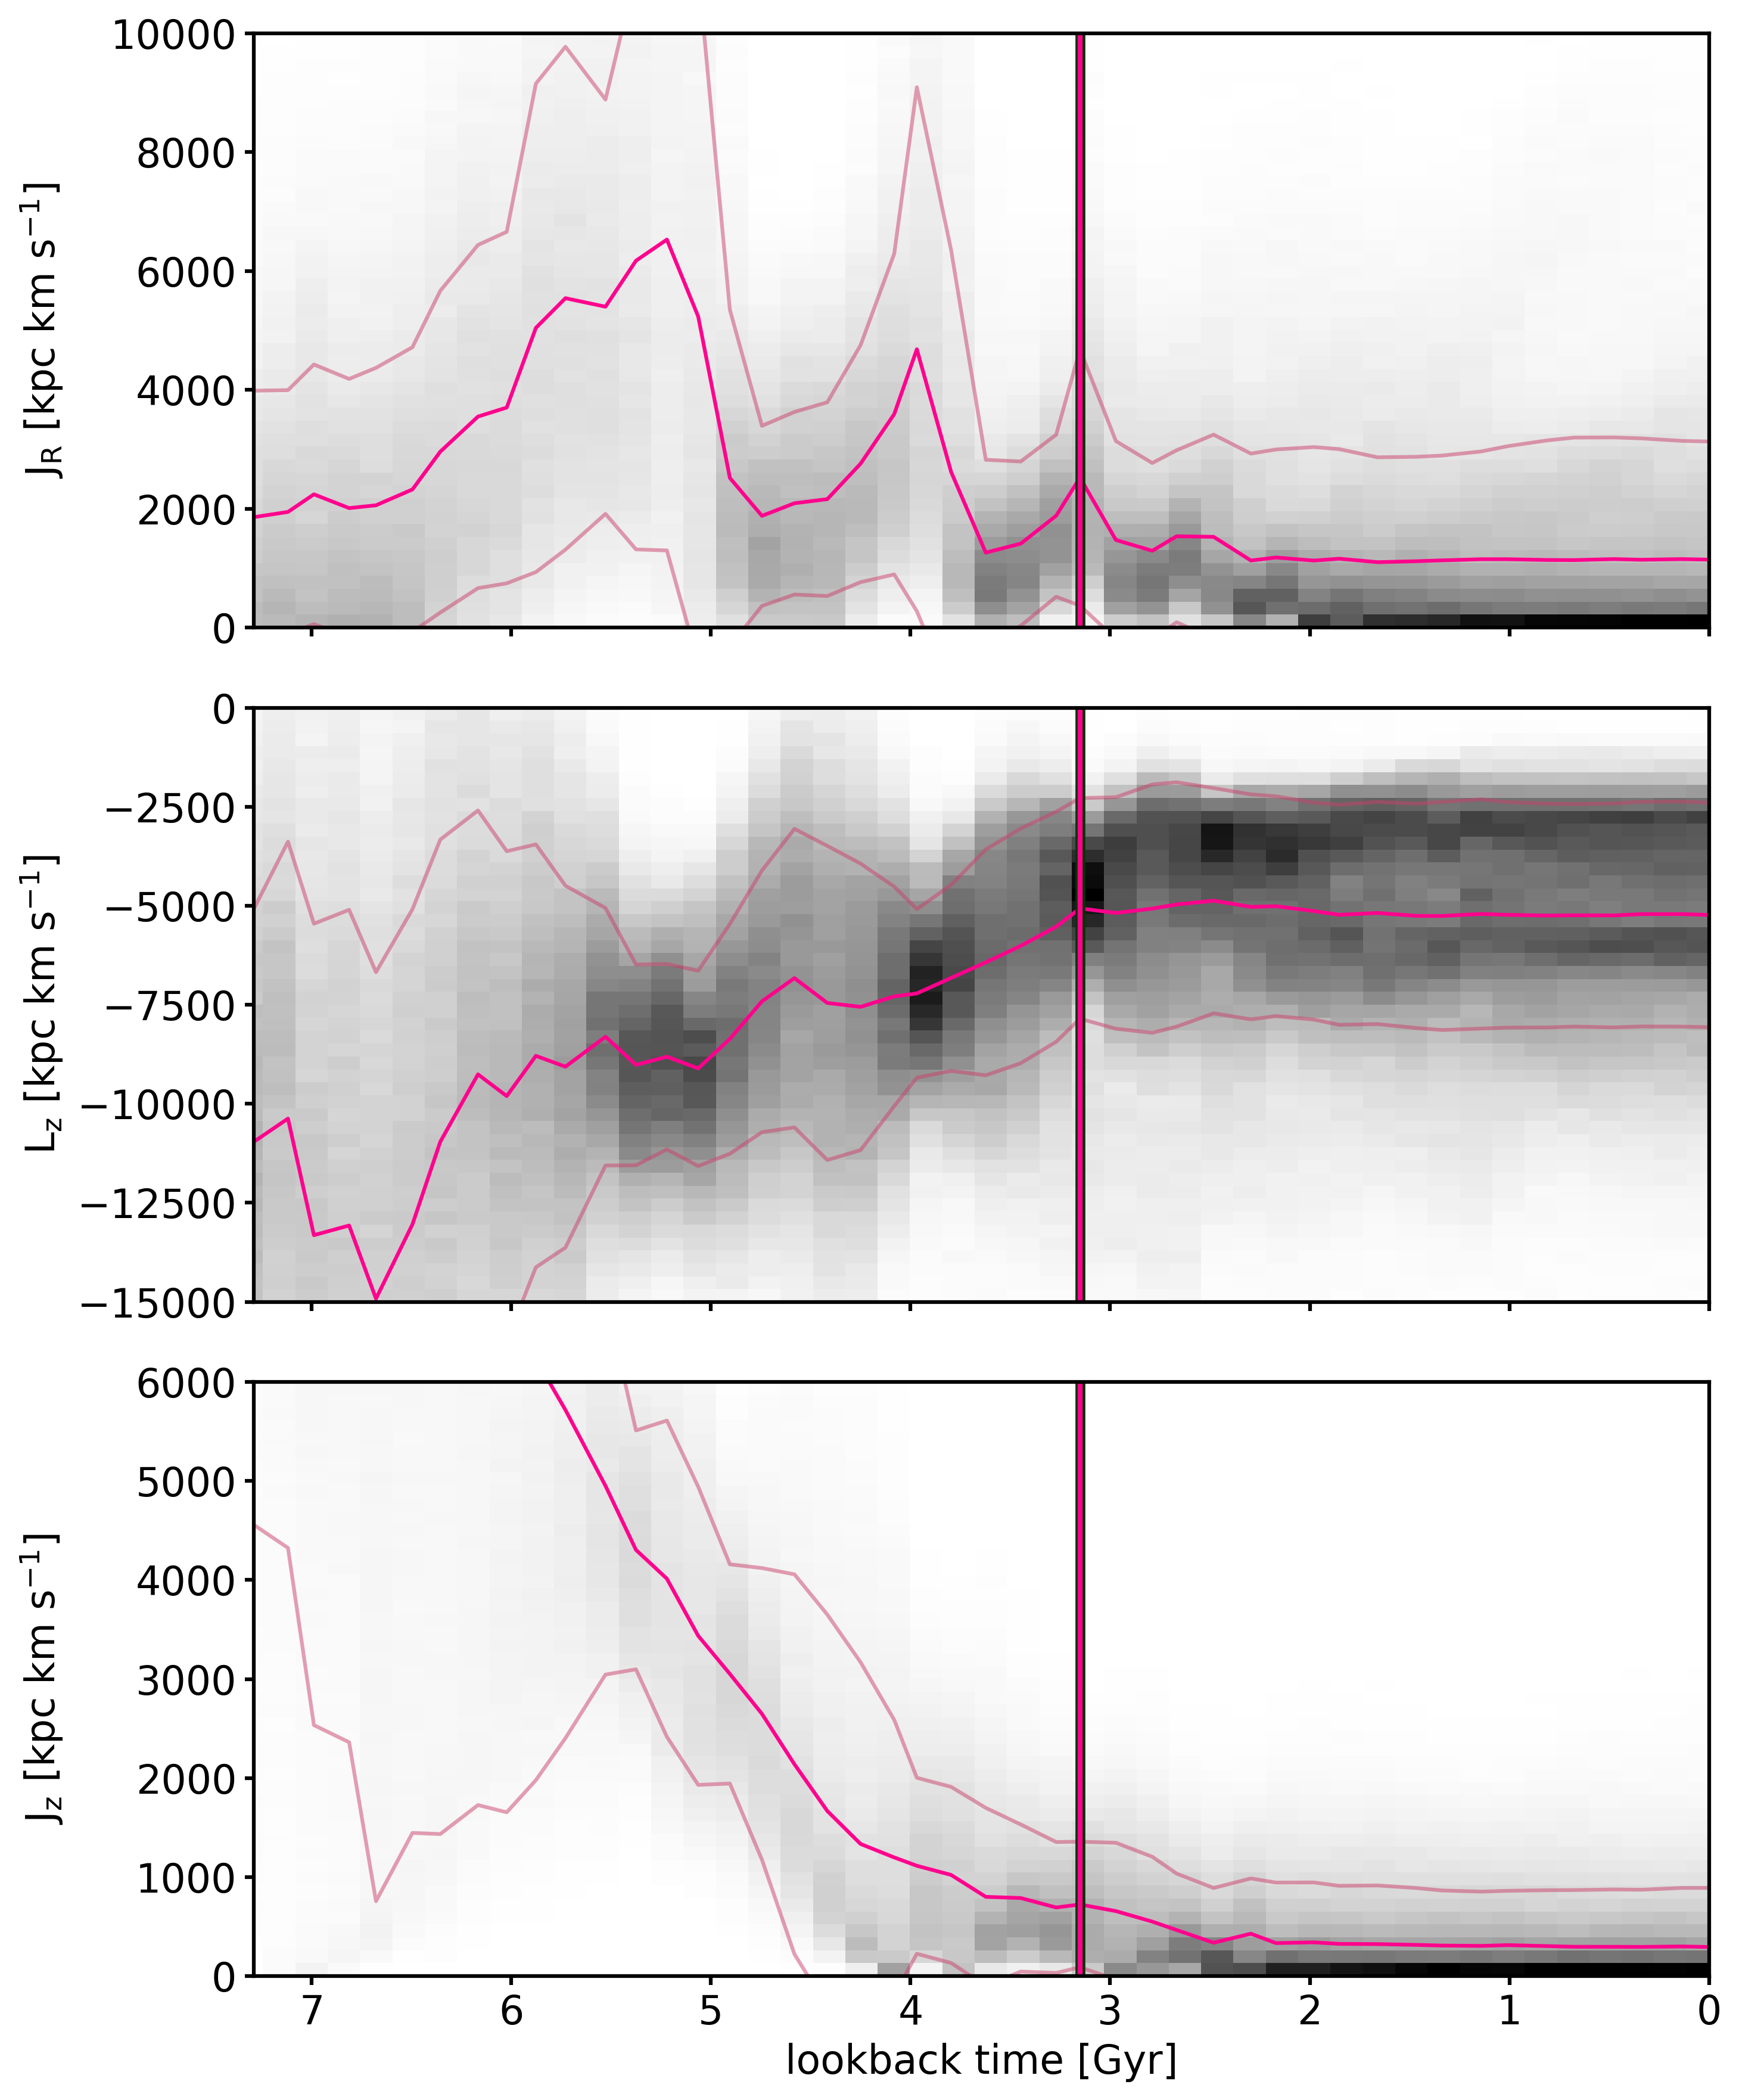
\includegraphics[width=\textwidth]{plots/Dynamics/prog2/action_time_evolution_wodisk_hist_mean.png}

	\caption{Evolution of actions of prog2 \acp{GC} over time. The pink vertical line indicates the time of the merger. The other pink lines follow the median (bright pink) and the standard deviation (light pink). \textit{Upper panel}: Radial action. \textit{Middle panel}: Angular momentum. \textit{Lower panel}: Vertical action. Before the merger, radial and vertical action were much higher and all three actions had higher standard deviations. With the merger, they have settled and$L_z$ and $J_z$ have a constant mean and standard deviation. $J_R$ has minimized in median and standard deviation shortly before the merger but since then both have increased again.}\label{fig:actions_time_evolution_prog2}
\end{figure}

\begin{figure}
\captionsetup{format=plain}
    \centering
	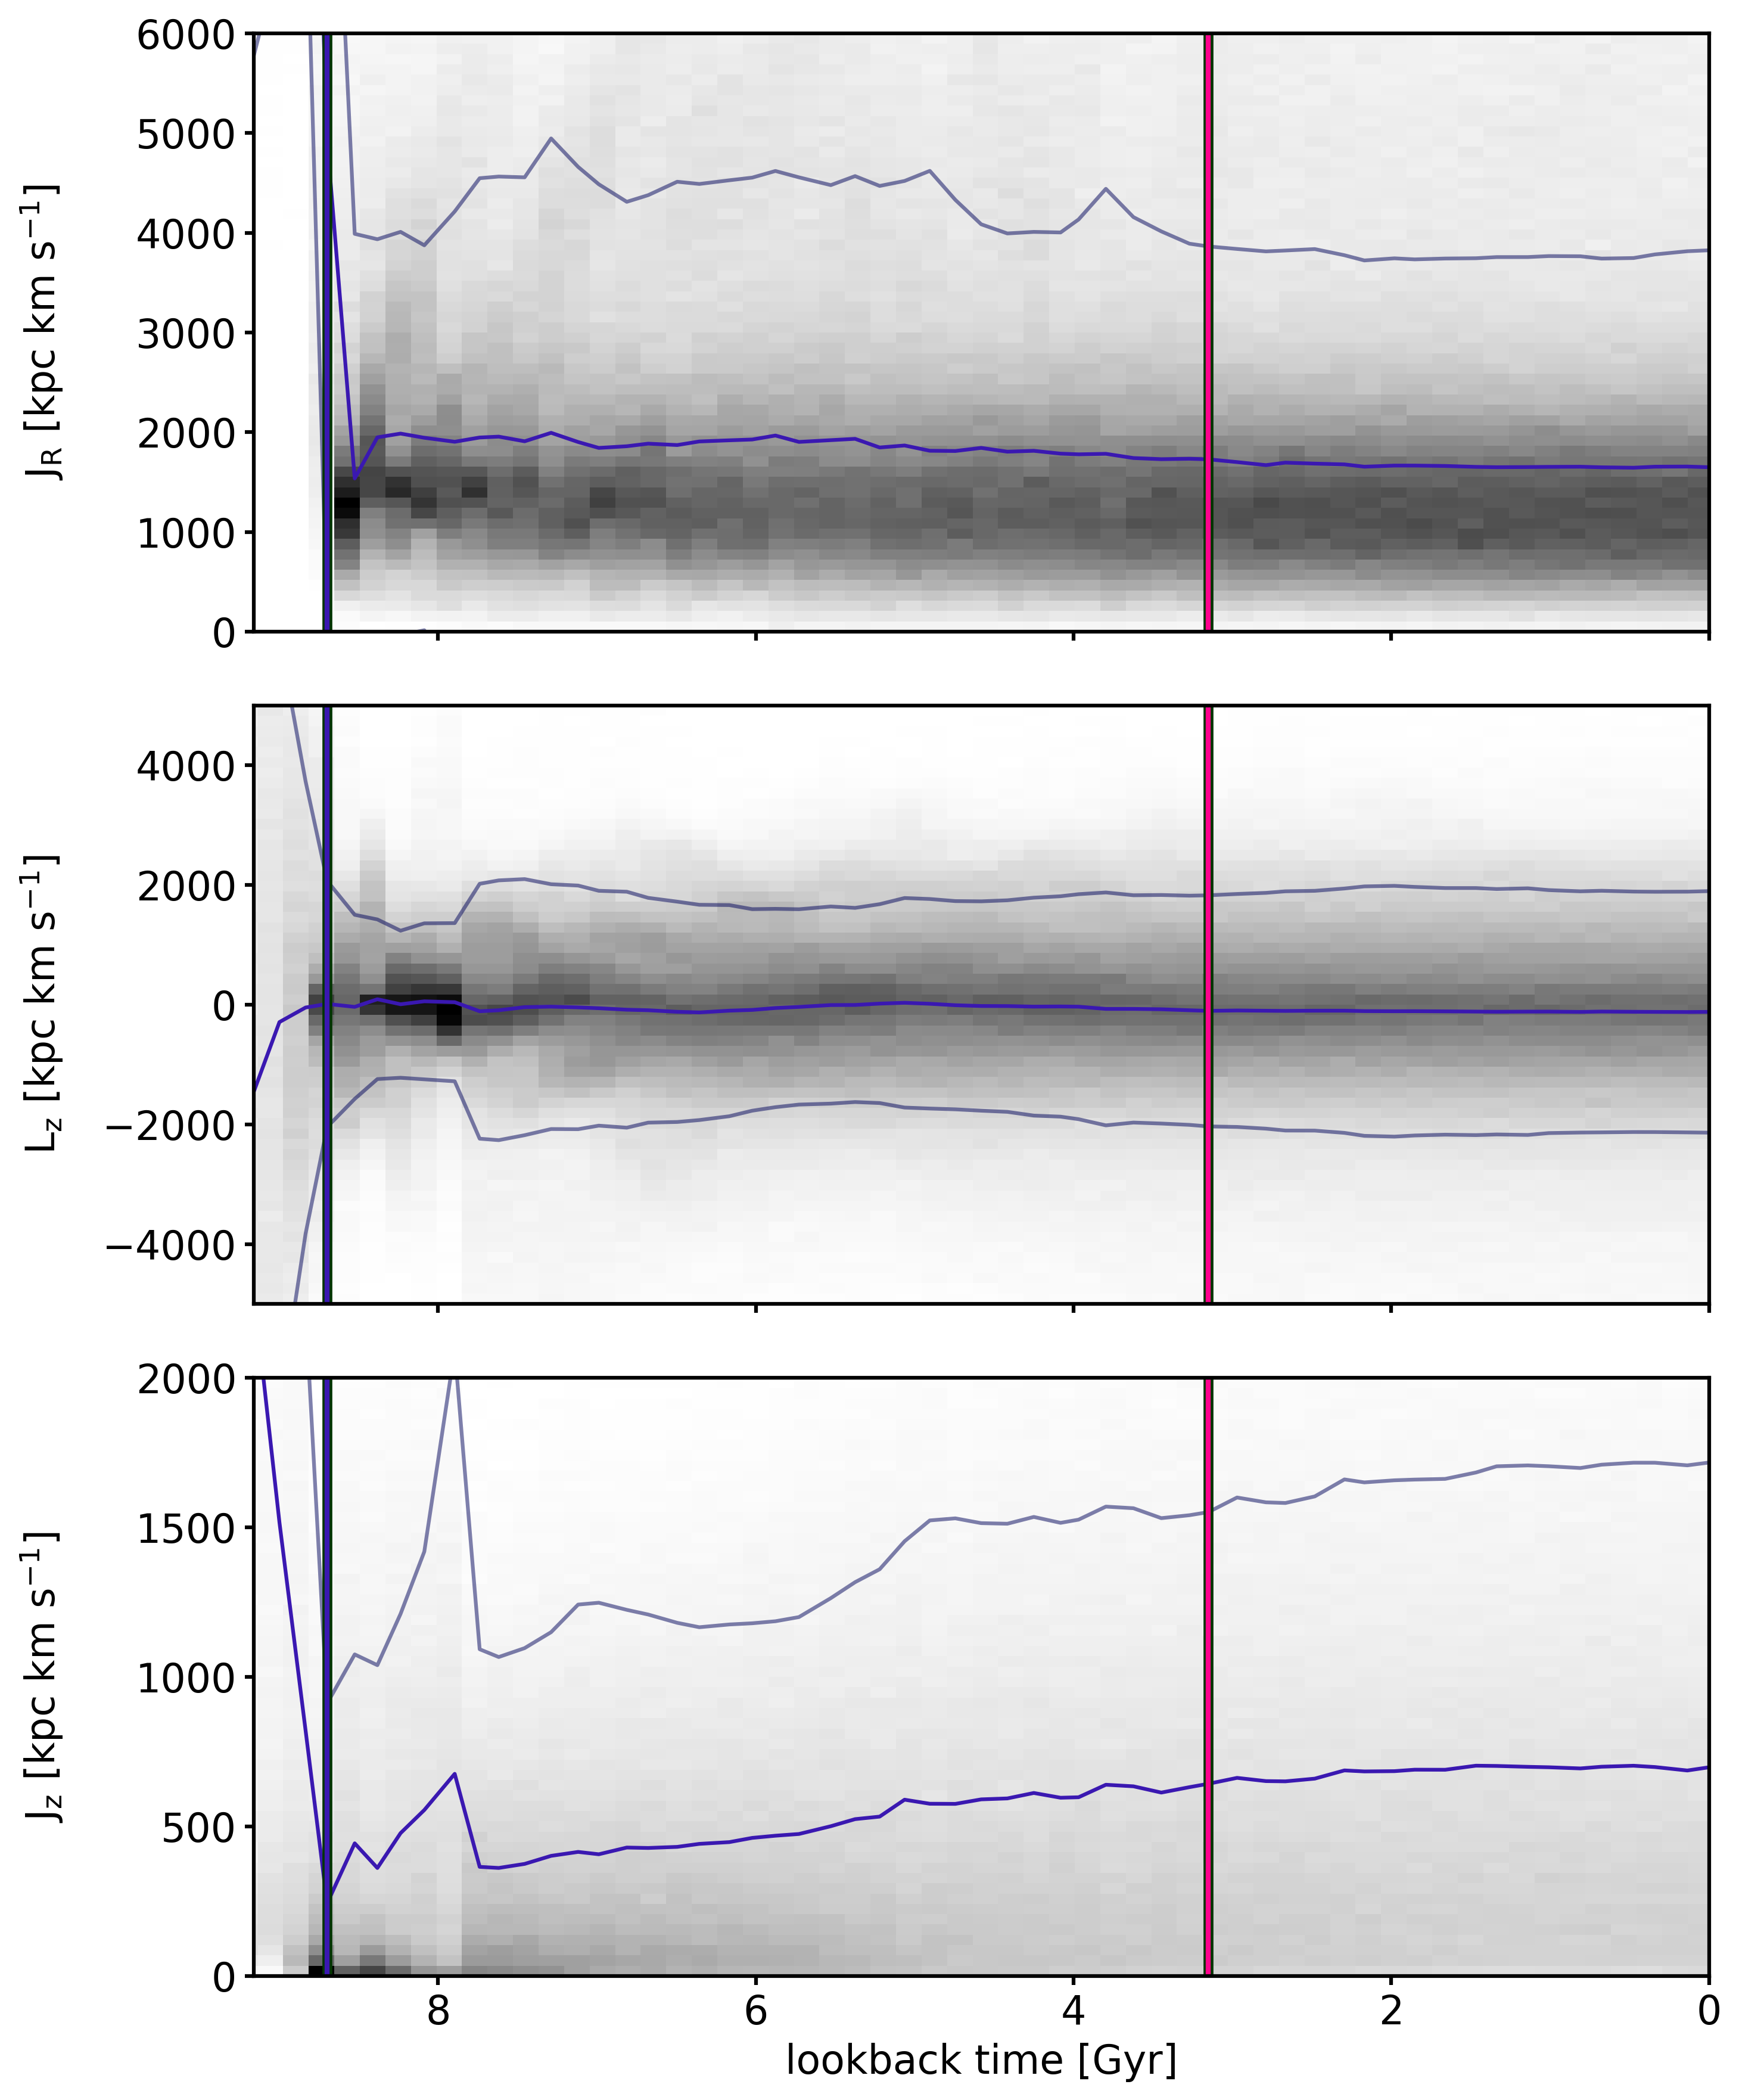
\includegraphics[width=\textwidth]{plots/Dynamics/prog3/action_time_evolution_wodisk_hist_mean.png}
    \caption{Time evolution of actions of prog3. The pink and blue lines indicate times of the mergers of prog2 and prog3, respectively. The other blue lines are the mean and the standard deviation. The panels are the same as in Figure \ref{fig:actions_time_evolution_prog2}. During the merger of prog3, $\overline{J}_z$ and $\sigma{_J_z}$ minimize. Shortly after the merger, the spread in $J_R$ and in $L_z$ minimizes while at the same time the median of $J_z$ and $\sigma{_J_z}$ rise steeply. The following evolution is rather constant for all actions with the spread slowly increasing.}\label{fig:actions_time_evolution_prog3}
\end{figure}

\begin{figure}[htbp]
\captionsetup{format=plain}
    \centering
	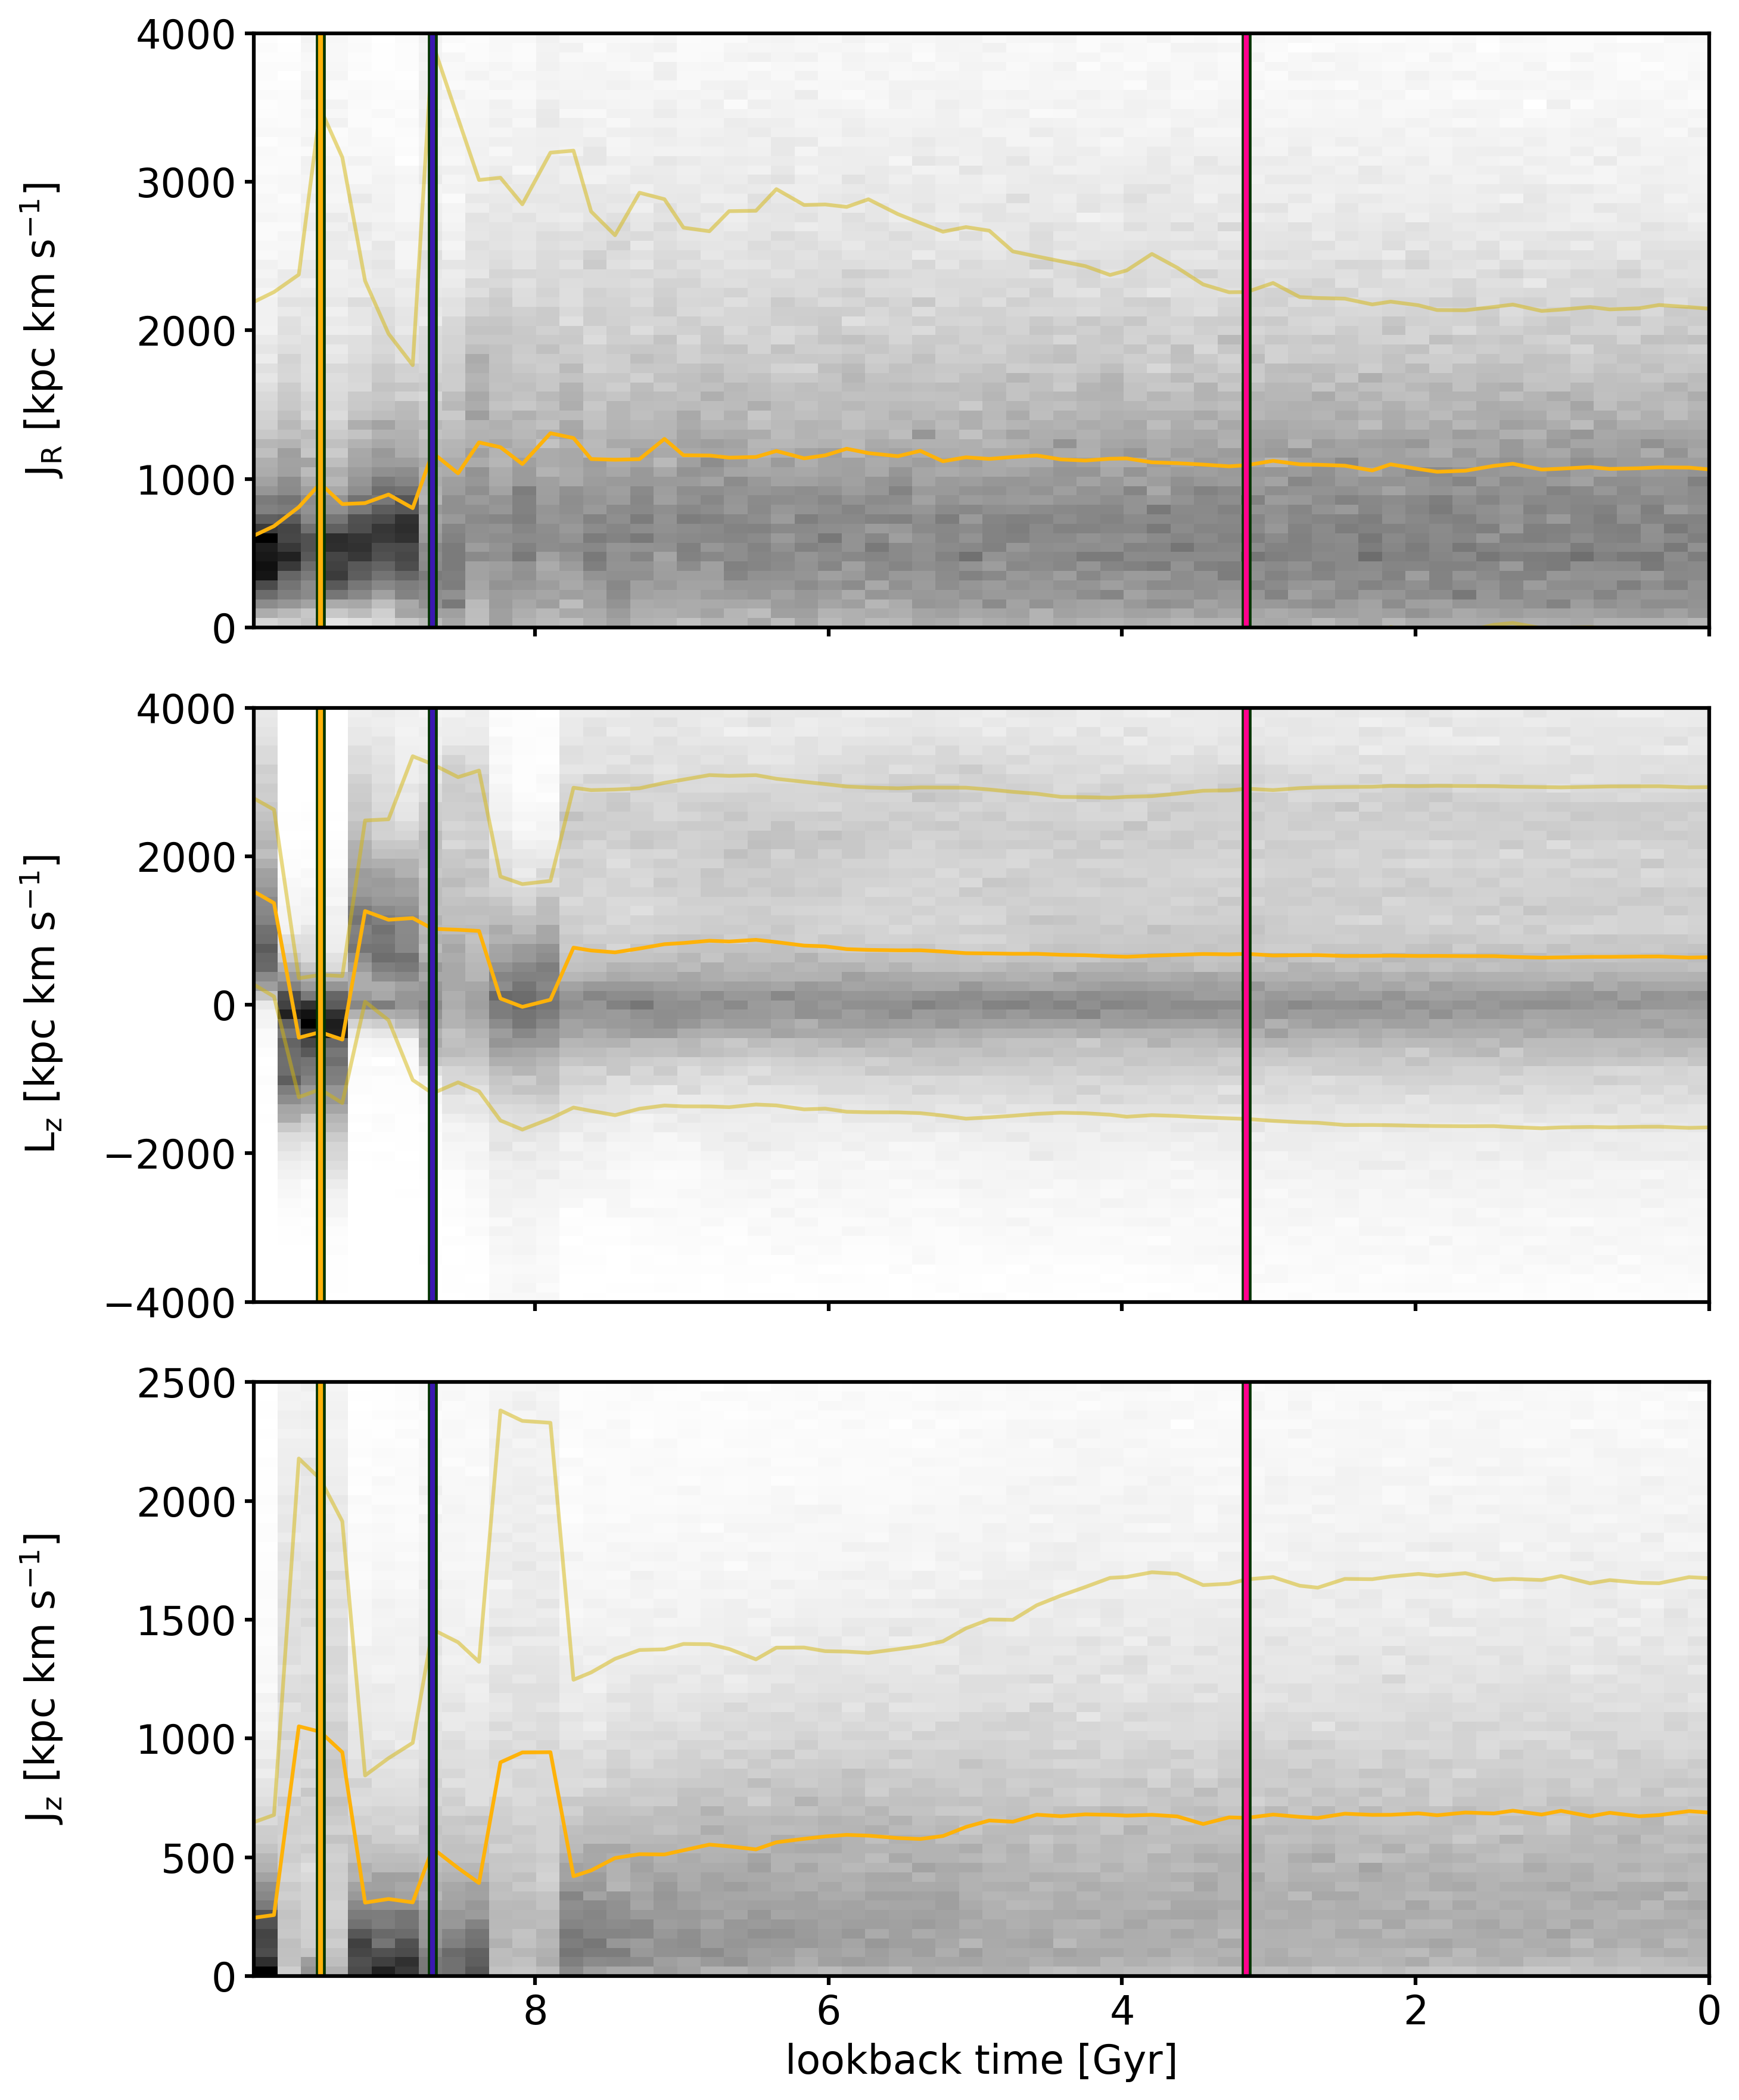
\includegraphics[width=\textwidth]{plots/Dynamics/prog4/action_time_evolution_wodisk_hist_mean.png}
    \caption{Prog4's \acp{GC} time evolution in action space. The pink, blue and yellow lines indicate times of the mergers of prog2, prog3 and prog4, respectively. The yellow lines are median and standard deviation. The panels are the same as in Figure \ref{fig:actions_time_evolution_prog2}. During the merger of prog4, radial and vertical actions have a steep rise while $L_z$ drops below 0. Something similar happens shortly after the merger of prog3. Since \SI{7.5}{Gyr} the actions stay constant and with the merger of prog2, the scatter in $J_R$ and $J_z$ becomes even less.}\label{fig:actions_time_evolution_prog4}
\end{figure}
In Figures \ref{fig:actions_time_evolution_prog2}, \ref{fig:actions_time_evolution_prog3} and \ref{fig:actions_time_evolution_prog4} we present these time evolutions for the \acp{GC} of prog2 / prog3 / prog4, respectively. For the prog2 \acp{GC}, Figure \ref{fig:actions_time_evolution_prog2}, we see nicely how before the merger the actions where very widely spread and towards the merger and especially afterwards their variance becomes smaller and the mean of each action stays constant. Since the merger, more significant clumping than in the last snapshot is not seen. In prog3, we find a strong clump shortly after the merger. The actions of prog4 are strongly varying shortly after the merger for about \SI{2}{Gyr} before they become steady.

\subsubsection{Mean best fit potential}\label{subsubsec:GCs_actions_time_mean_right_pot}
The idea that actions do not change over time is valid in a static or only slowly varying potential. Even though the overall action distribution did not change to much over time, we will see in Section \ref{subsec:box_GCs} that individual orbits vary drastically over time. Therefore, we need to test if the assumption of having a potential which only varies slowly is true. A rather simple execution is to calculate the action evolution in a static potential and check if it varies from our results. To do so, we calculate the mean of each potential parameter since the last big merger event (prog2). 
\begin{figure}[htbp]
\captionsetup{format=plain}
    \centering
	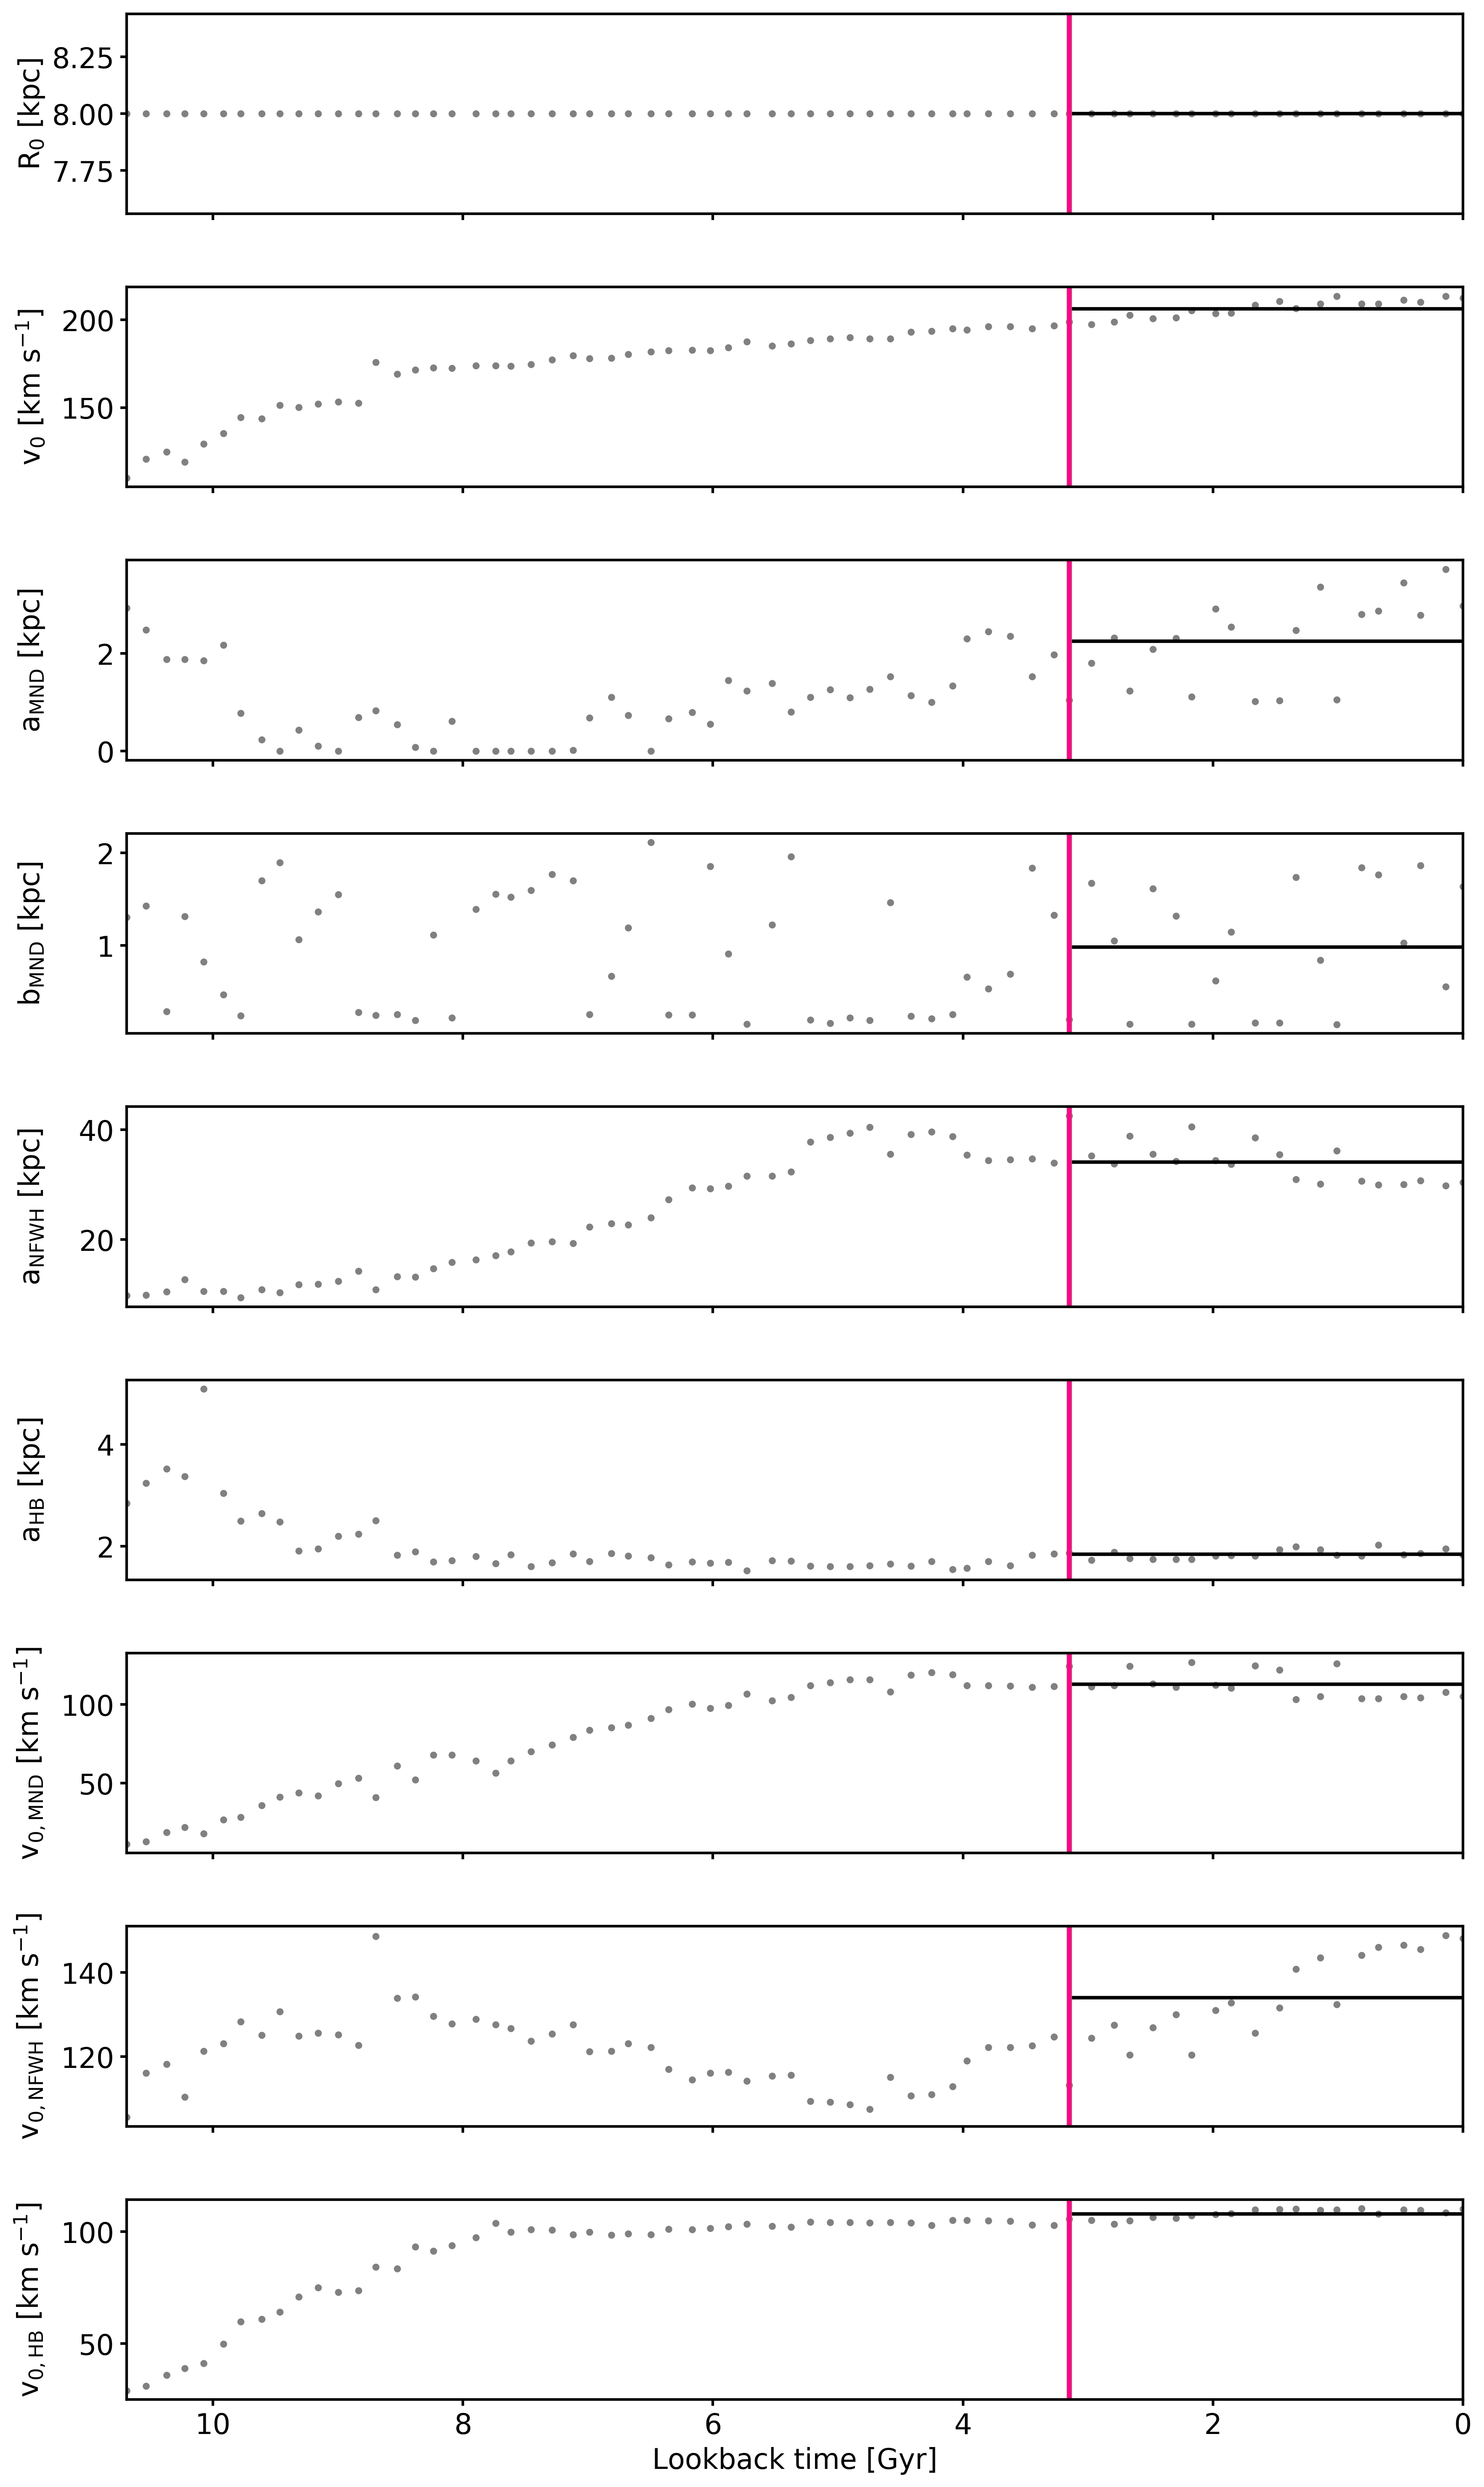
\includegraphics[width=0.8\textwidth]{plots/Dynamics/mean_pot/potential_evolution_with_mean_jan19.png}
    \caption{Time evolution of best fit potential parameters and their mean values since the merger of prog2 (indicated in pink). The scatter of disk and halo parameters is relatively large while the bulge parameters stay constant in this time range. We use this potential to compare the actions in the slowly varying potential (Figure \ref{fig:pot_val_evol}) to the actions in this static potential.}\label{fig:potential_mean_evolution}
\end{figure}
In Figure \ref{fig:potential_mean_evolution}, we show again the parameter evolution and the mean value for each which we use to set up the static gravitational potential. Since we have large scatter in the disk and halo parameters it is interesting to see if ignoring their slopes has any consequences on the action calculation. 
\begin{figure}[htbp]
\captionsetup{format=plain}
    \begin{subfigure}[c]{0.48\textwidth}
    \centering
    	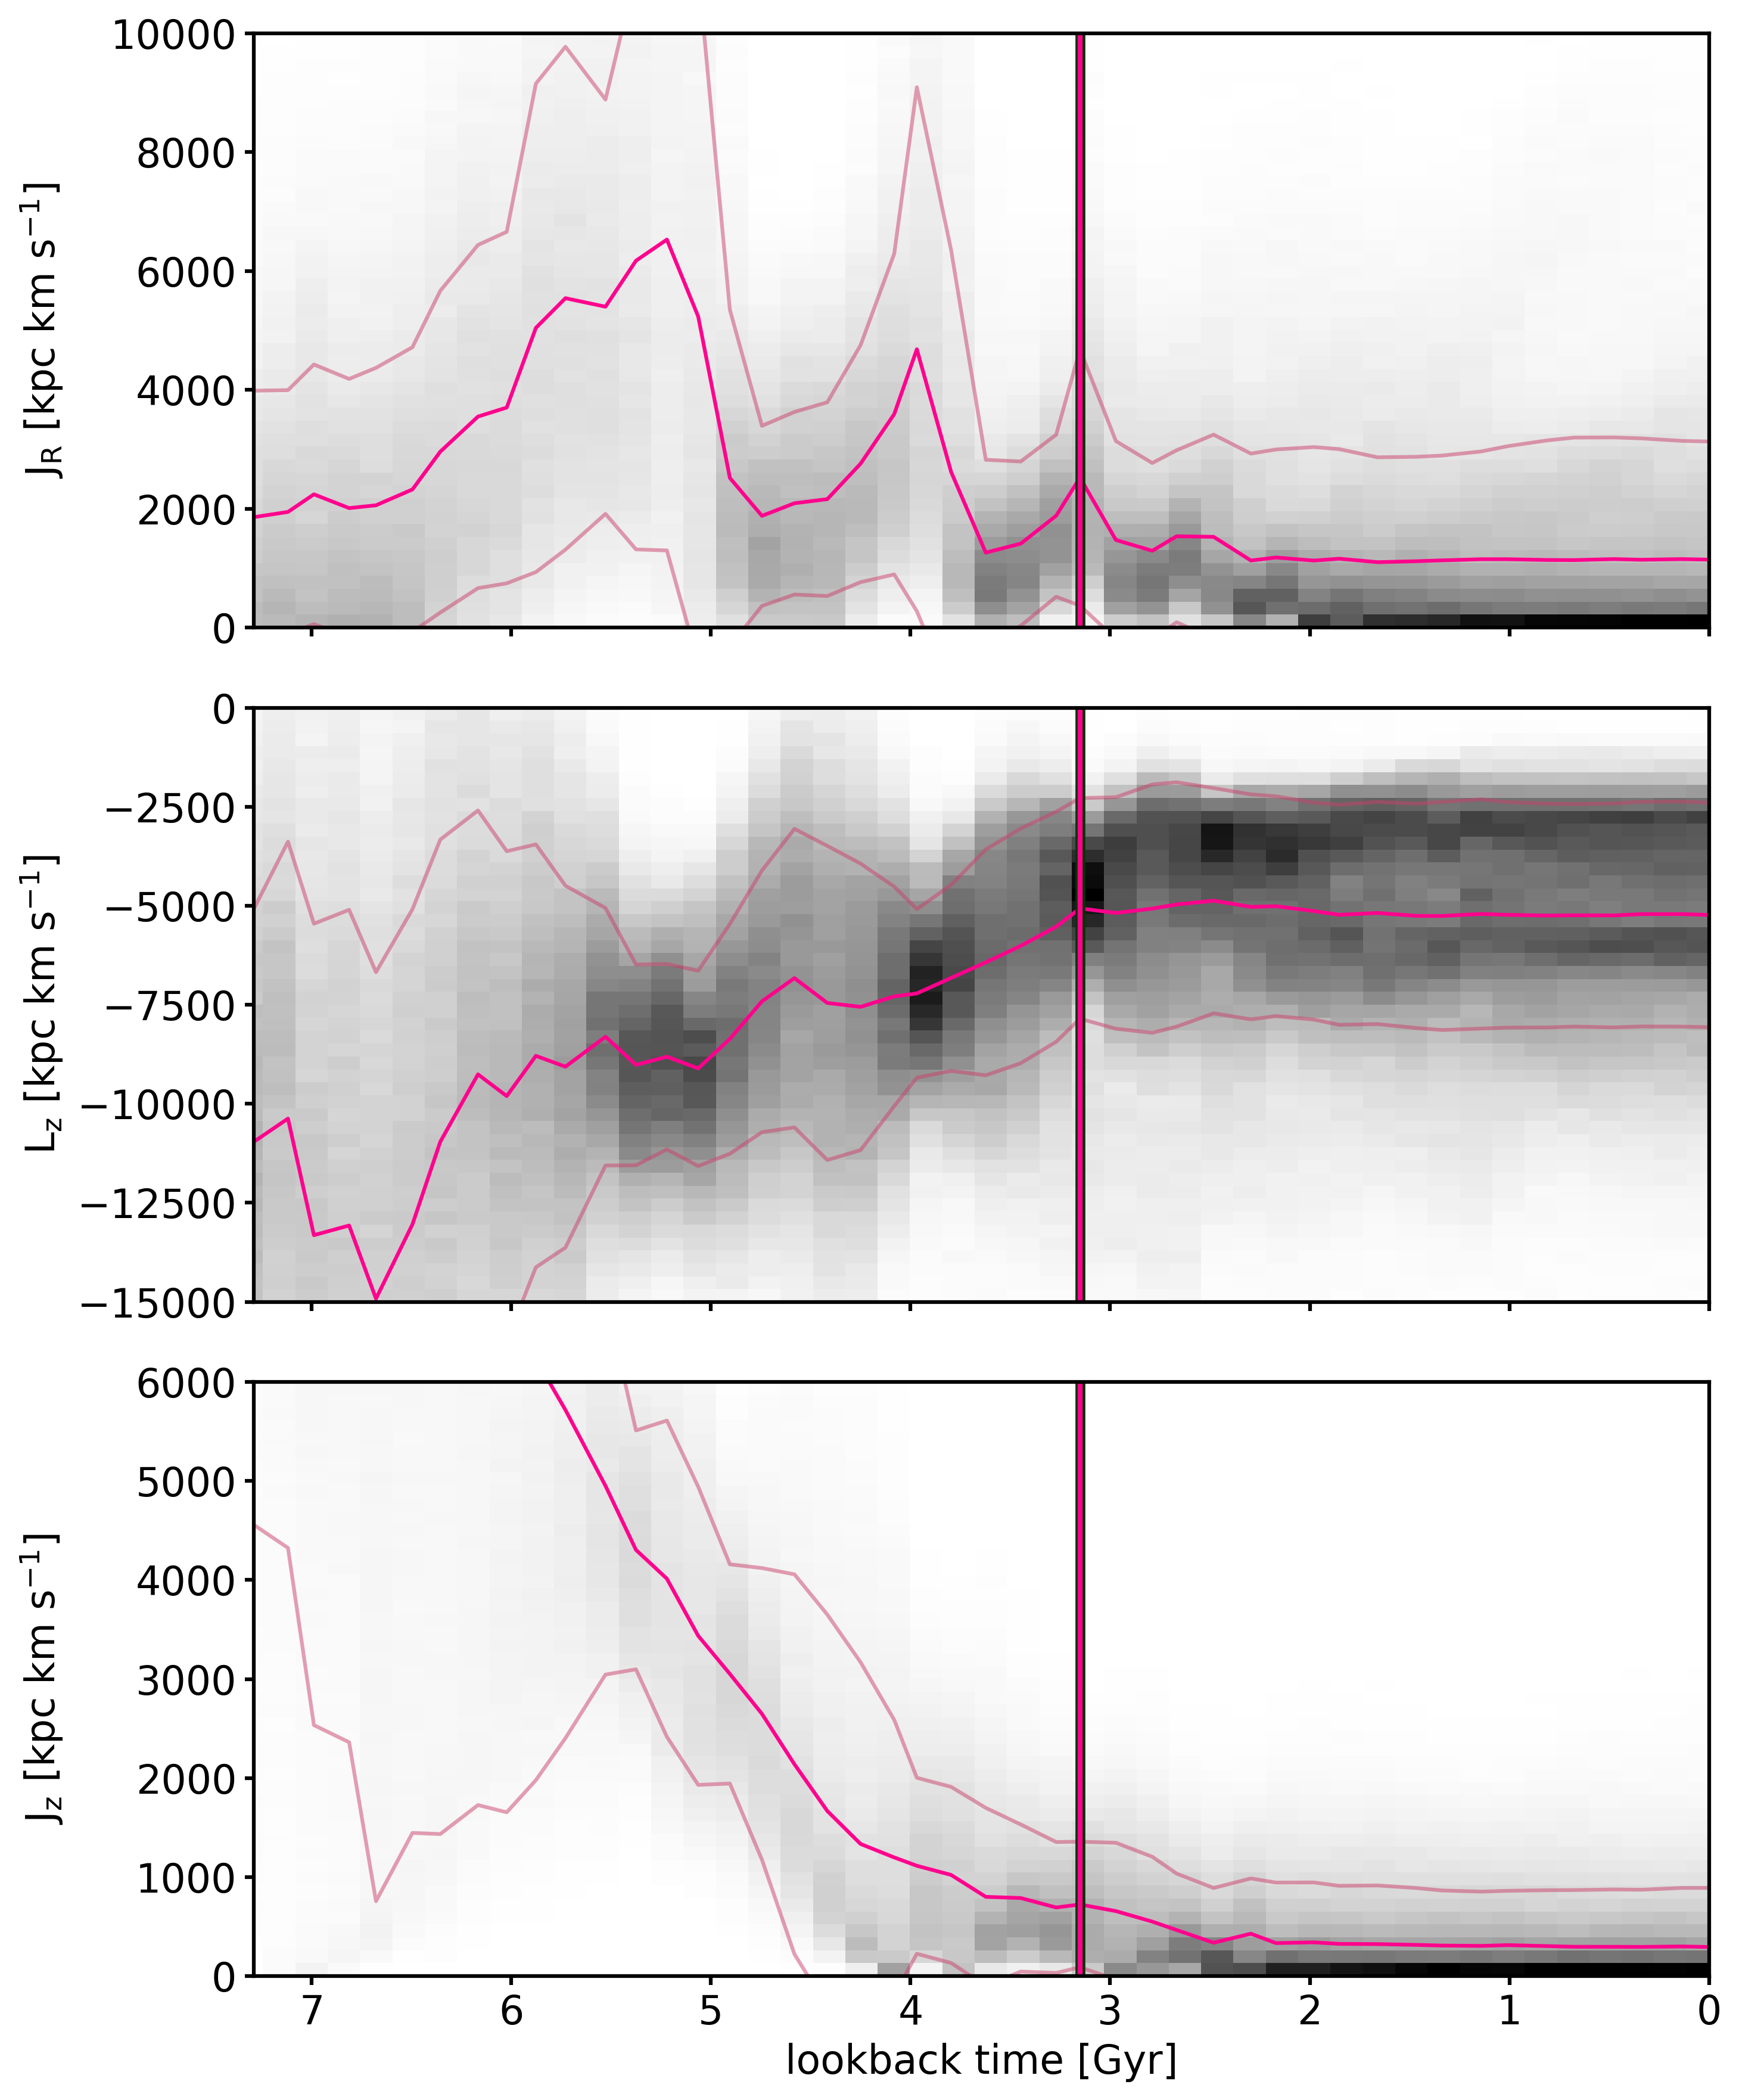
\includegraphics[width=\textwidth]{plots/Dynamics/prog2/action_time_evolution_wodisk_hist_mean.png}
    \end{subfigure}
    ~
    \begin{subfigure}[c]{0.48\textwidth}
    \centering
	    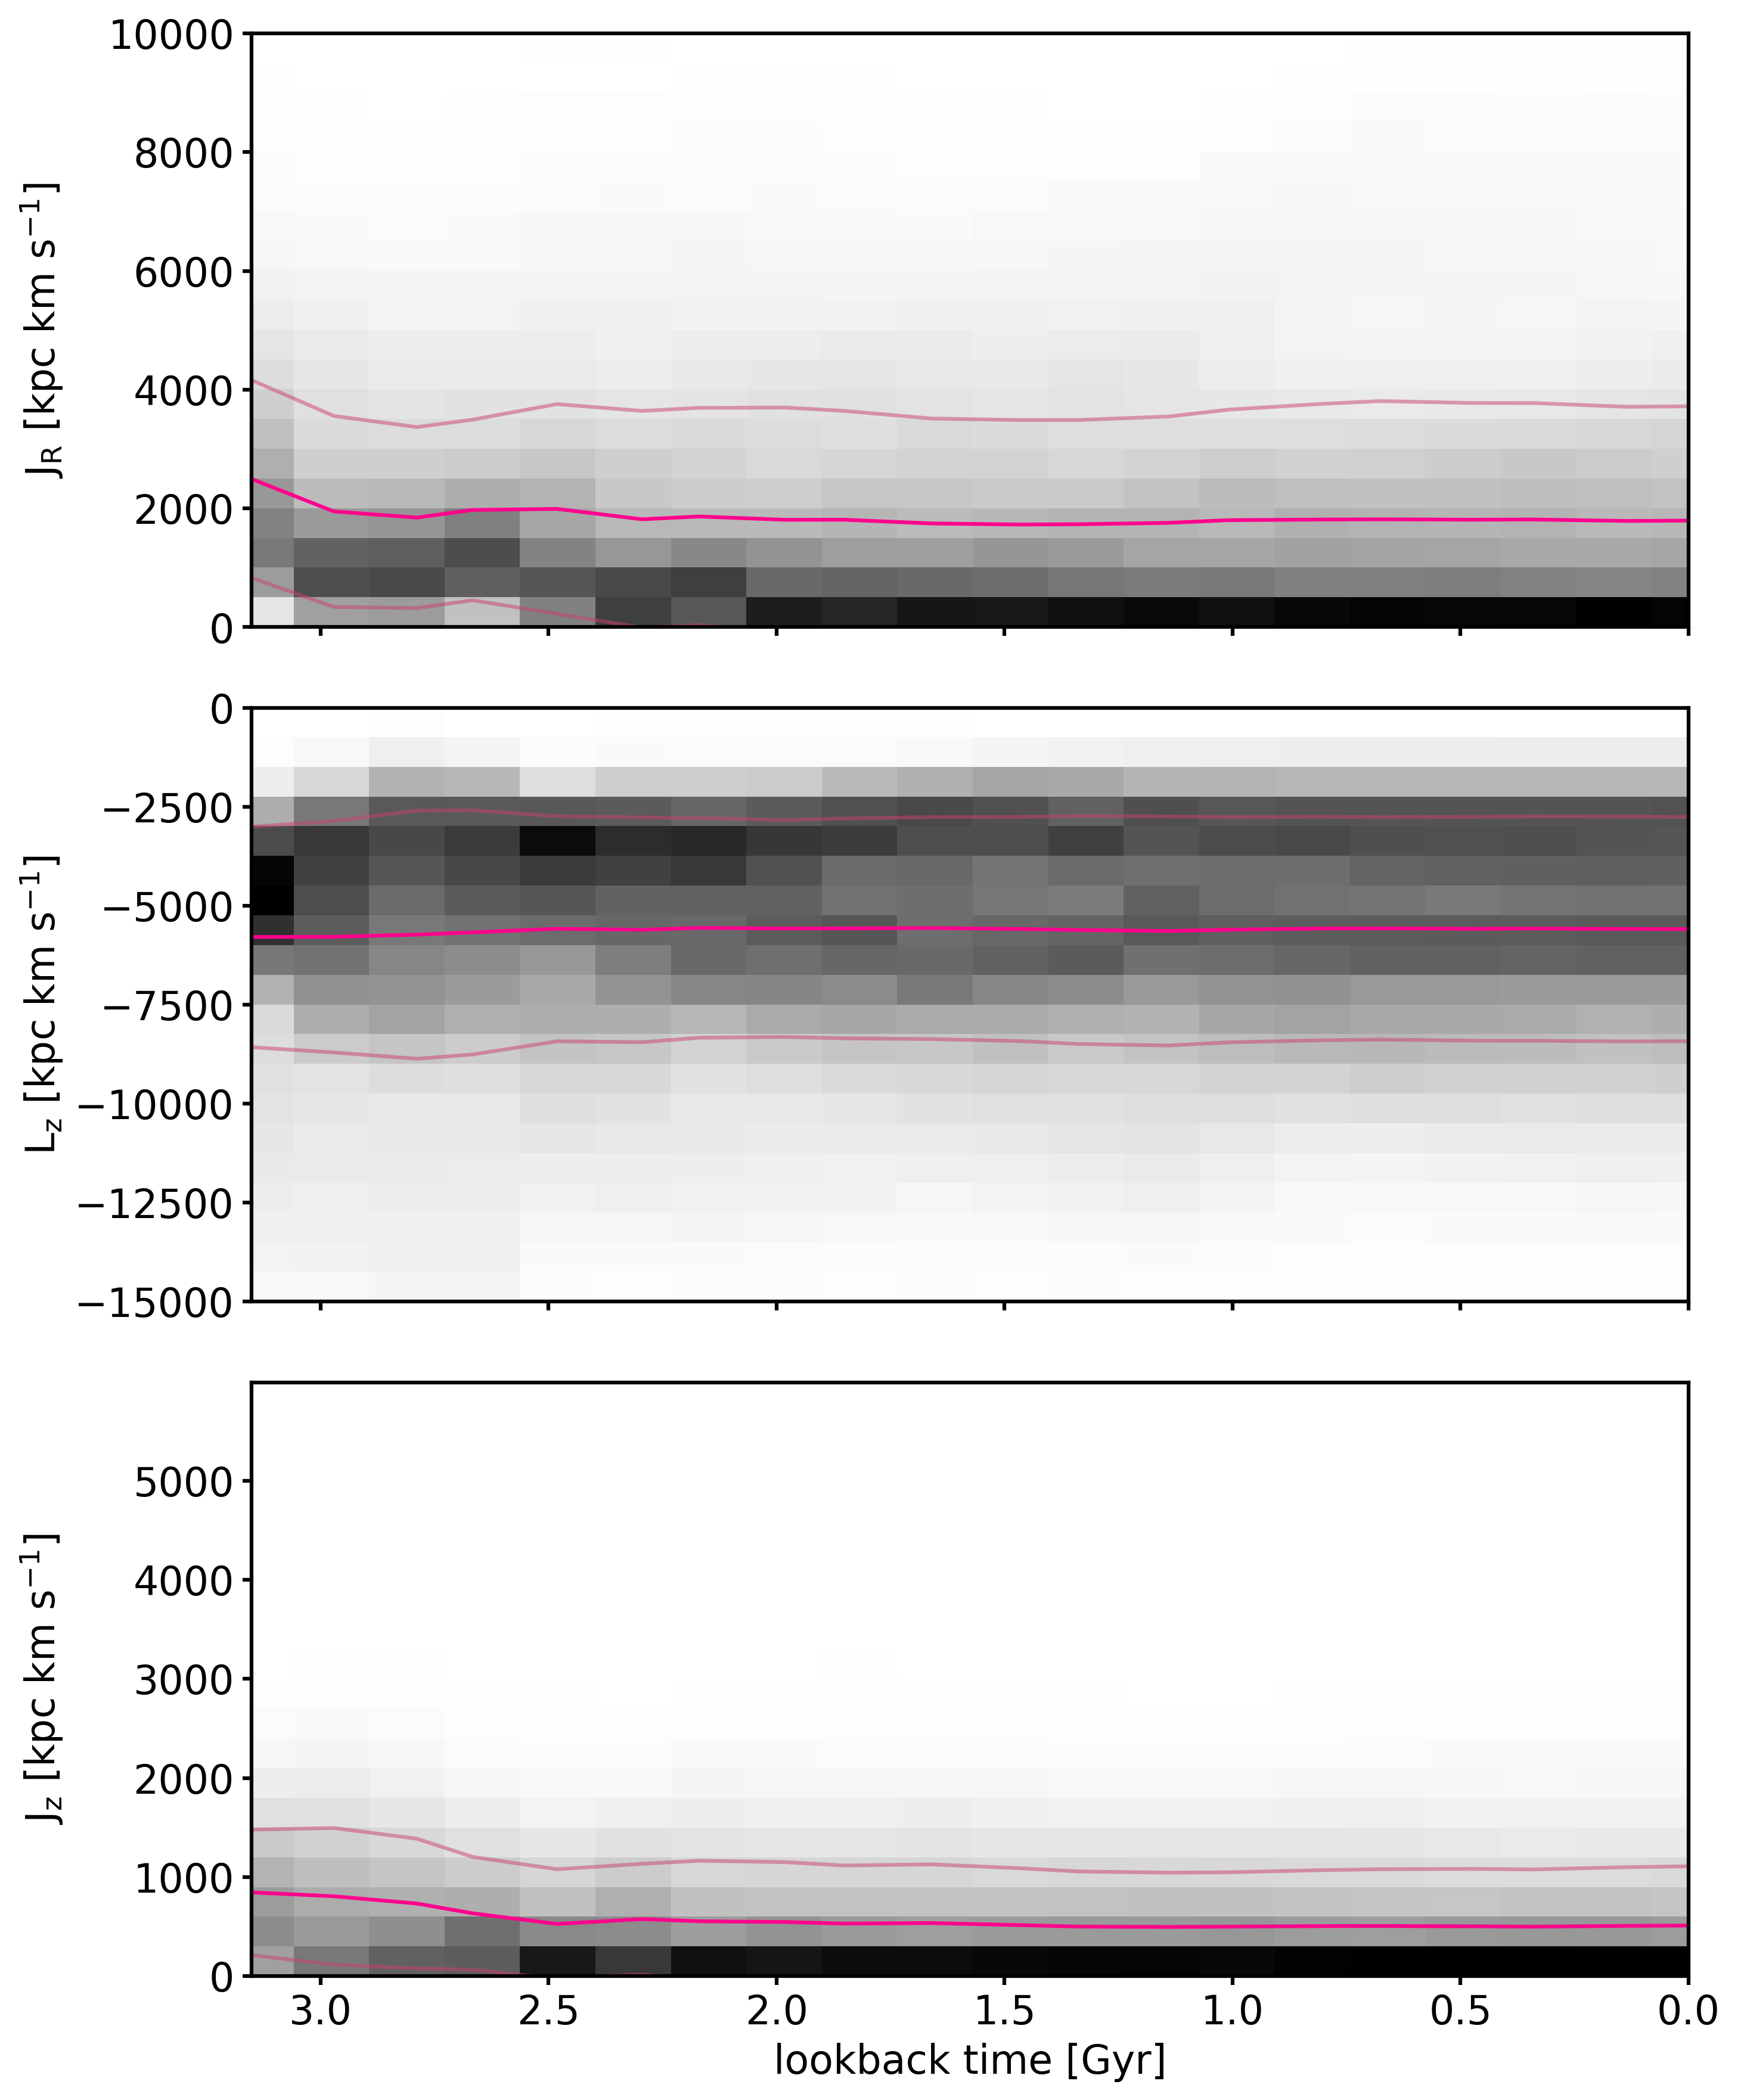
\includegraphics[width=\textwidth]{plots/Dynamics/prog2/action_wodisk_time_evolution_hist_mean_static_pot.png}
    \end{subfigure}
    \caption{Same as Figure \ref{fig:actions_time_evolution_prog2}, only for a constant potential since the merger of prog2.\textcolor{red}{update with new selected GCs coming}}\label{fig:comparison_actions_time_evolution_mean_pot_prog2}
\end{figure}
In the time regime since the last merger we calculated the actions of each progenitor group in the static potential. In Figure \ref{fig:comparison_actions_time_evolution_mean_pot_prog2}, we compare the \acp{GC} of prog2 in action space in the varying potential (left) and the static potential (right). There is no difference in the time evolution visible. We did the same for the \acp{GC} of prog3 and prog4 and they also show no differences. Therefore, the assumption of having a slowly evolving potential can be considered correct.
\iffalse
\begin{figure}
\captionsetup{format=plain}
    \centering
	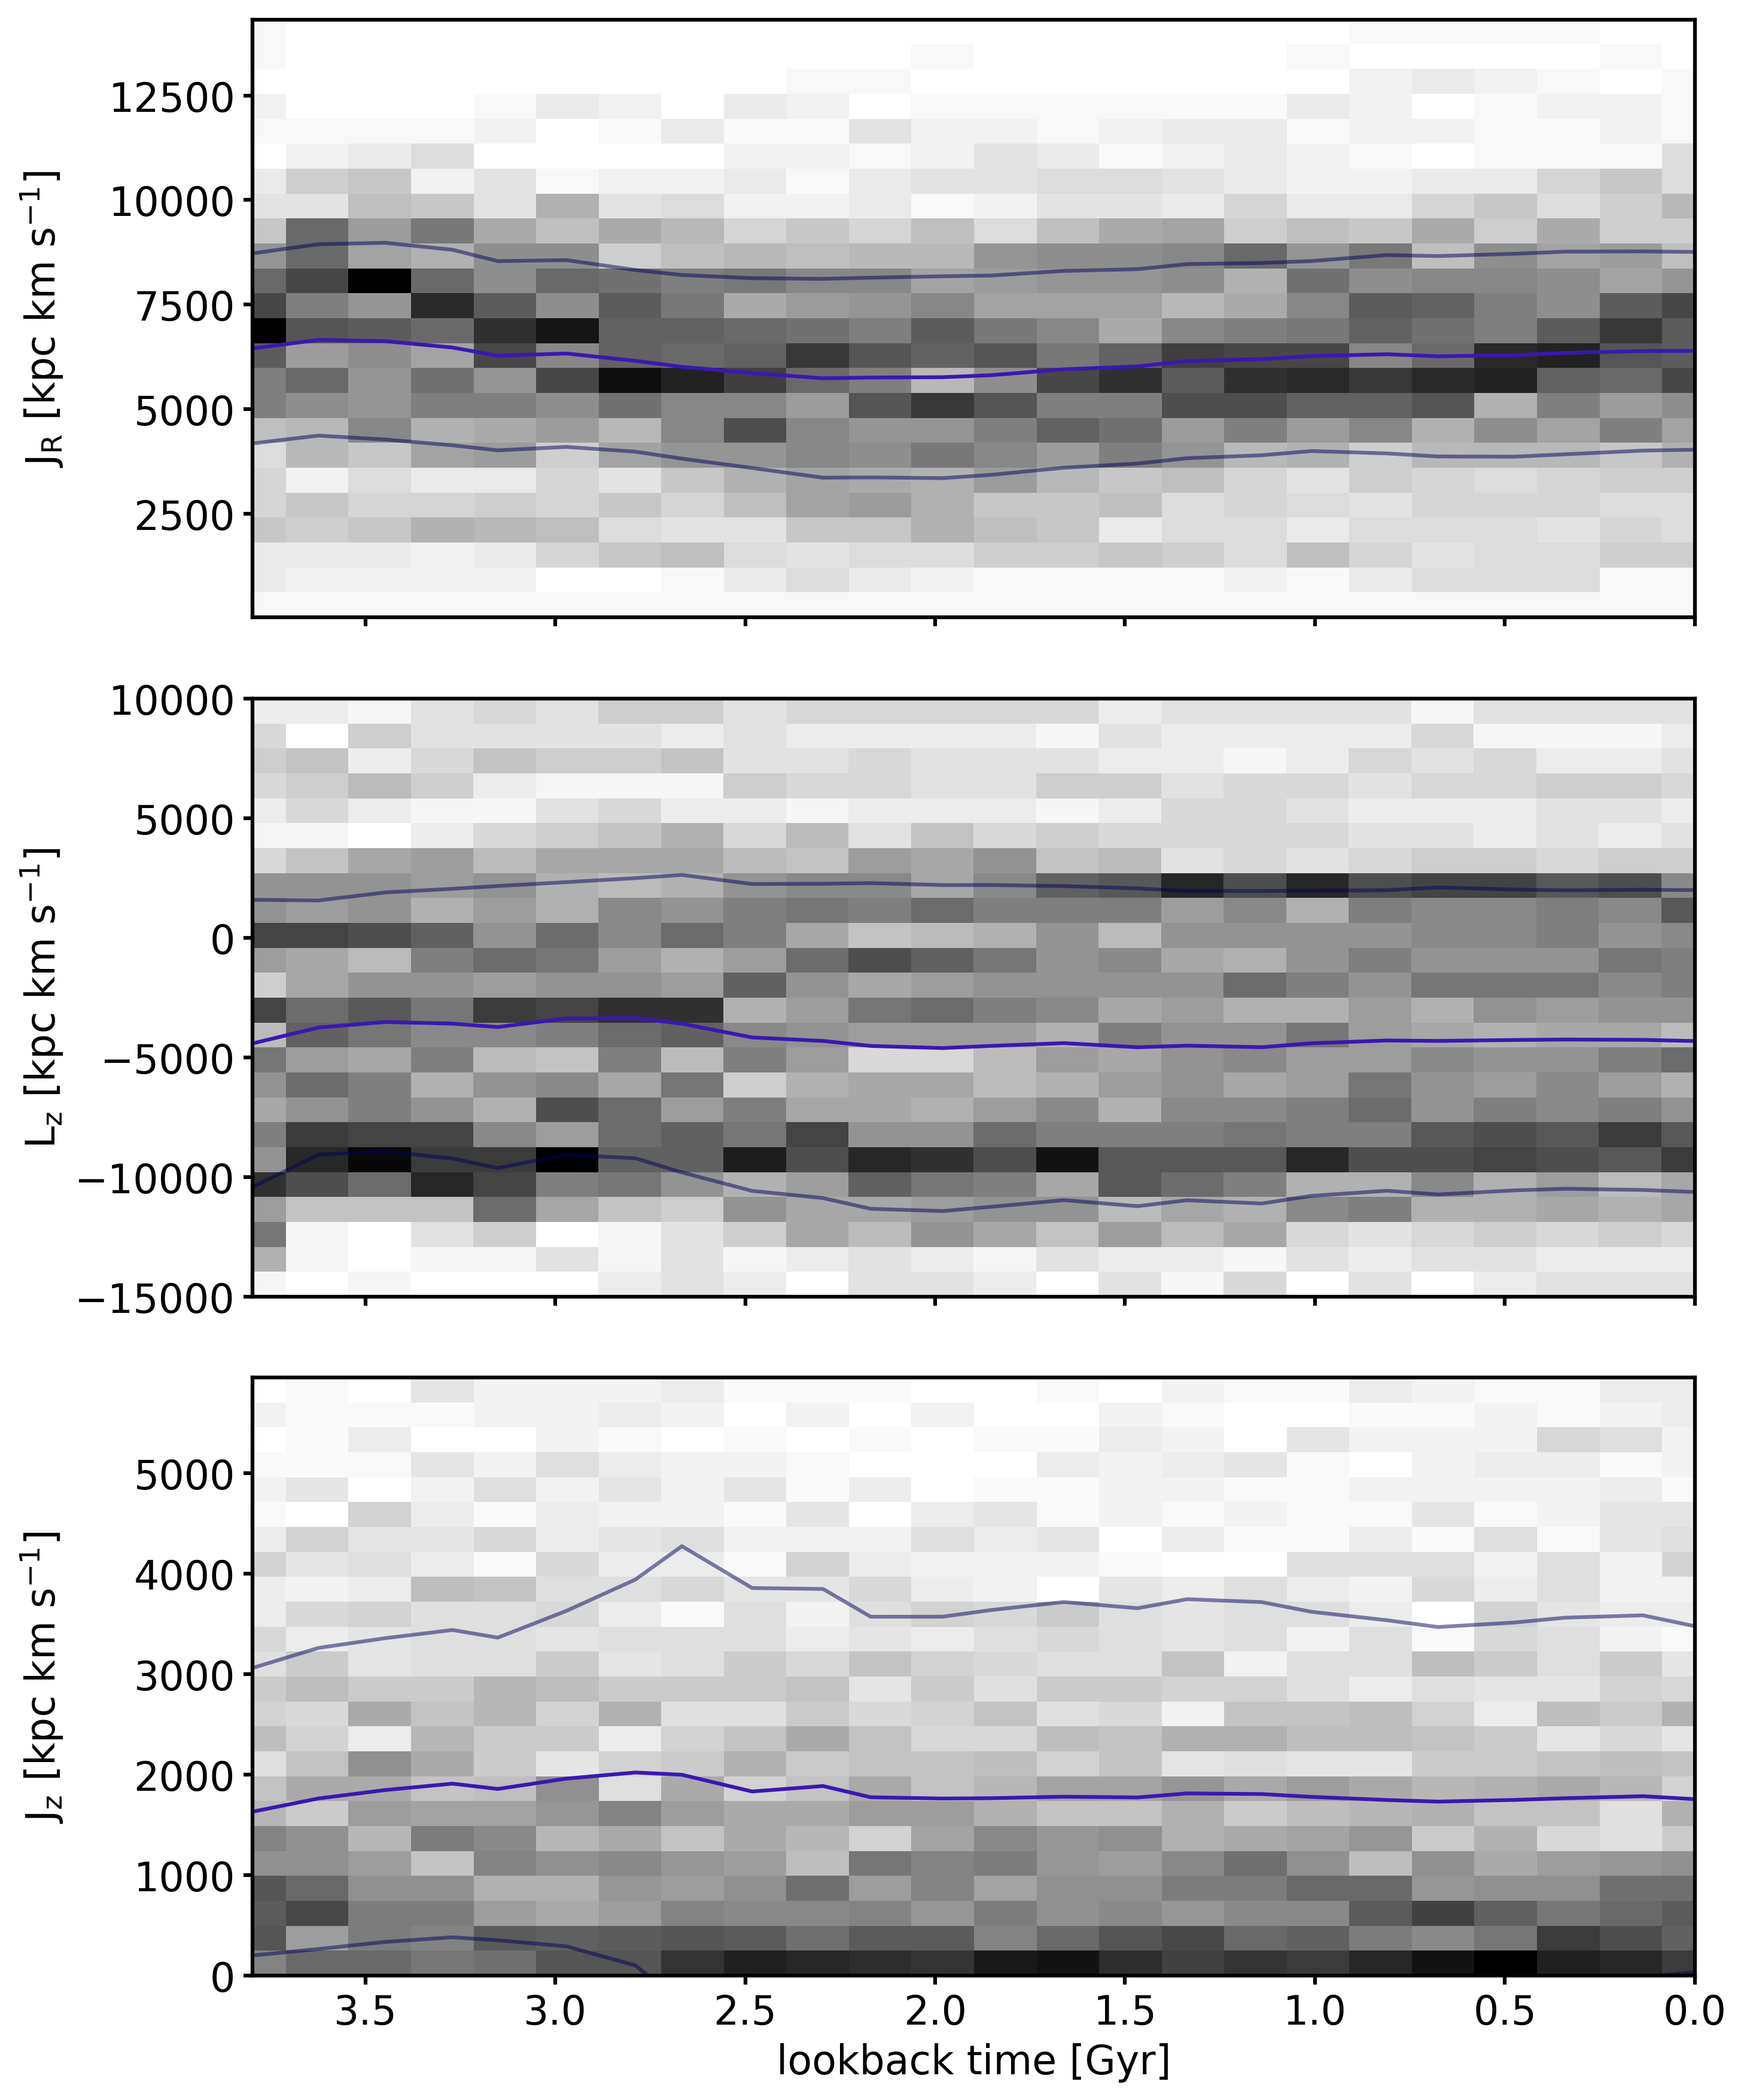
\includegraphics[width=\textwidth]{plots/Dynamics/mean_pot/action_time_evolution_hist_mean_prog3.png}
    \caption{Same as Figure \ref{fig:actions_time_evolution_prog3}, only for a constant potential since the merger of prog2.}\label{fig:actions_time_evolution_mean_pot_prog3}
\end{figure}

\begin{figure}[htbp]
\captionsetup{format=plain}
    \centering
	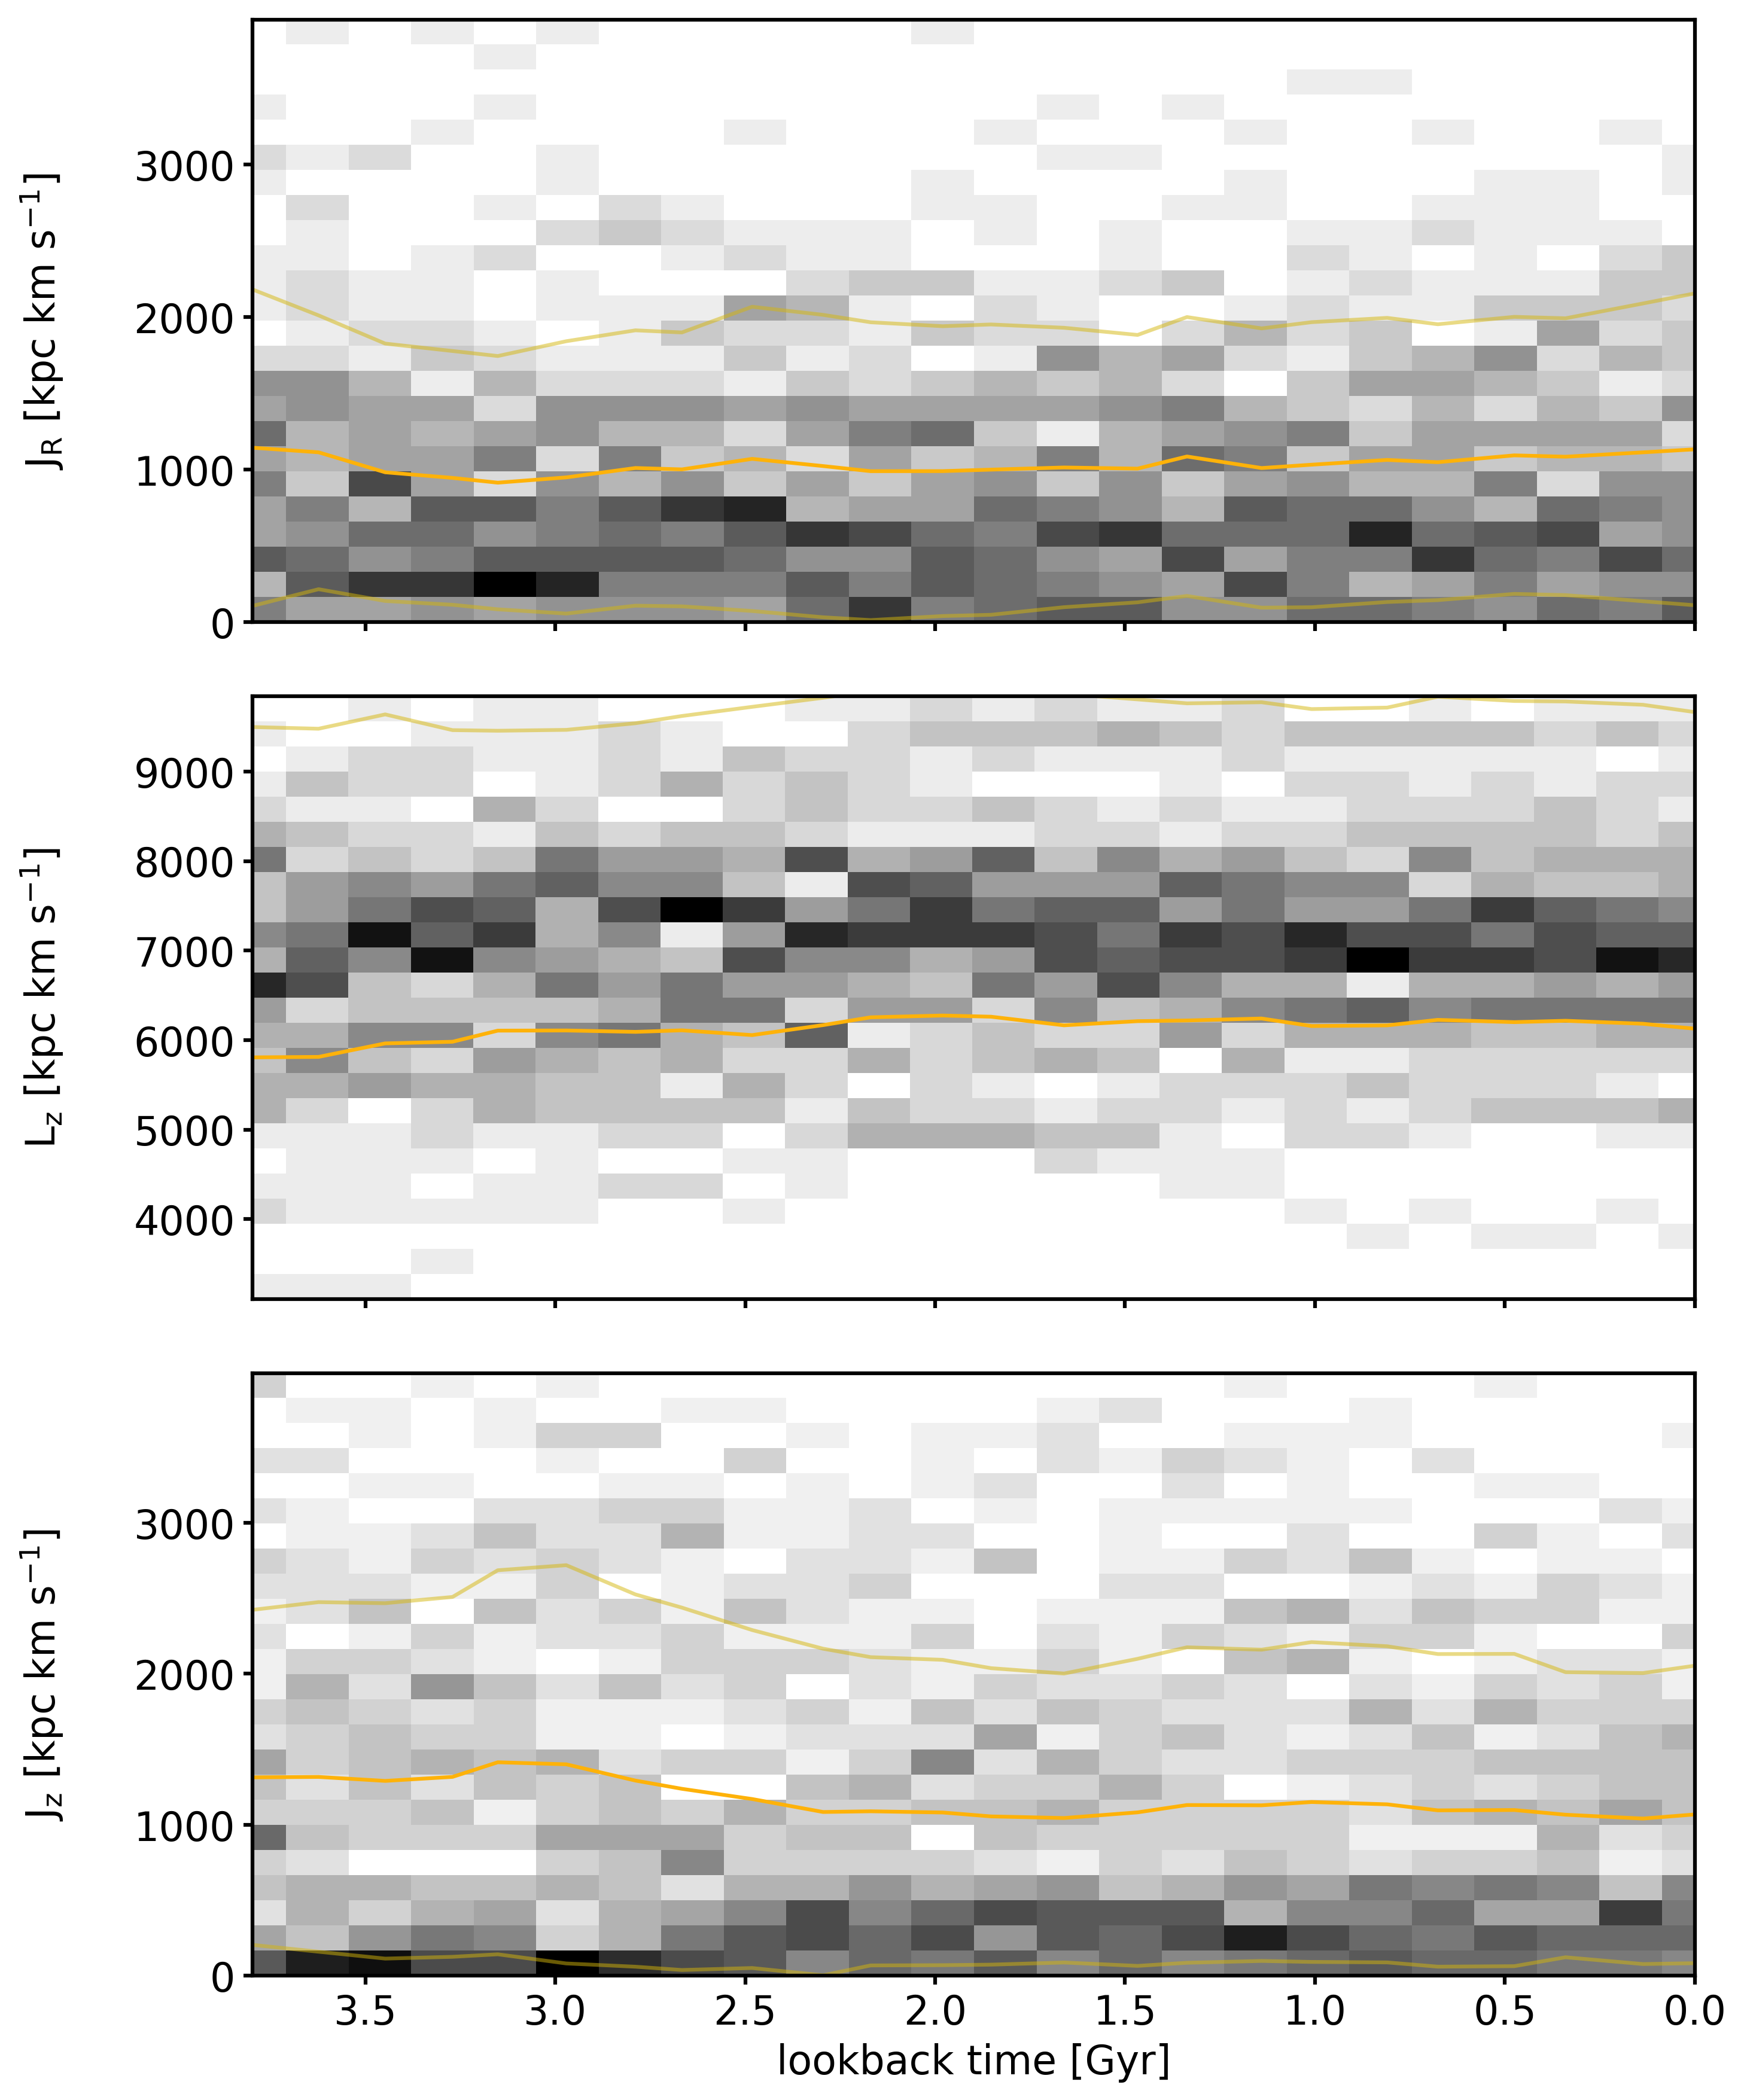
\includegraphics[width=\textwidth]{plots/Dynamics/mean_pot/action_time_evolution_hist_mean_prog4.png}
    \caption{Same as Figure \ref{fig:actions_time_evolution_prog4}, only for a constant potential since the merger of prog2.}\label{fig:actions_time_evolution_mean_pot_prog4}
\end{figure}
\fi

\subsubsection{Energy evolution}\label{subsubsec:energy_evol}
Another assumption under which we calculated the radial and vertical actions were the use of St\"ackel potentials. To test if variations and the missing of clumpiness could be due to numerical problems in this approach we can have a look at the other \ac{IoM}, angular momentum and energy. Since $L_z$ was rather constant in Figures \ref{fig:actions_time_evolution_prog2} - \ref{fig:actions_time_evolution_prog2} and \ref{fig:comparison_actions_time_evolution_mean_pot_prog2} we now evaluate the energy. It is calculated according to Equation \ref{eq:energy_hamiltonian} where $v = \Sigma v_i$. We can derive the energy directly from the data by taking the potential value from the simulation and we compare it to our potential model. The kinematic term of Equation \ref{eq:energy_hamiltonian} is identical for data and model.

\begin{figure}[htbp]
\captionsetup{format=plain}
    \centering
	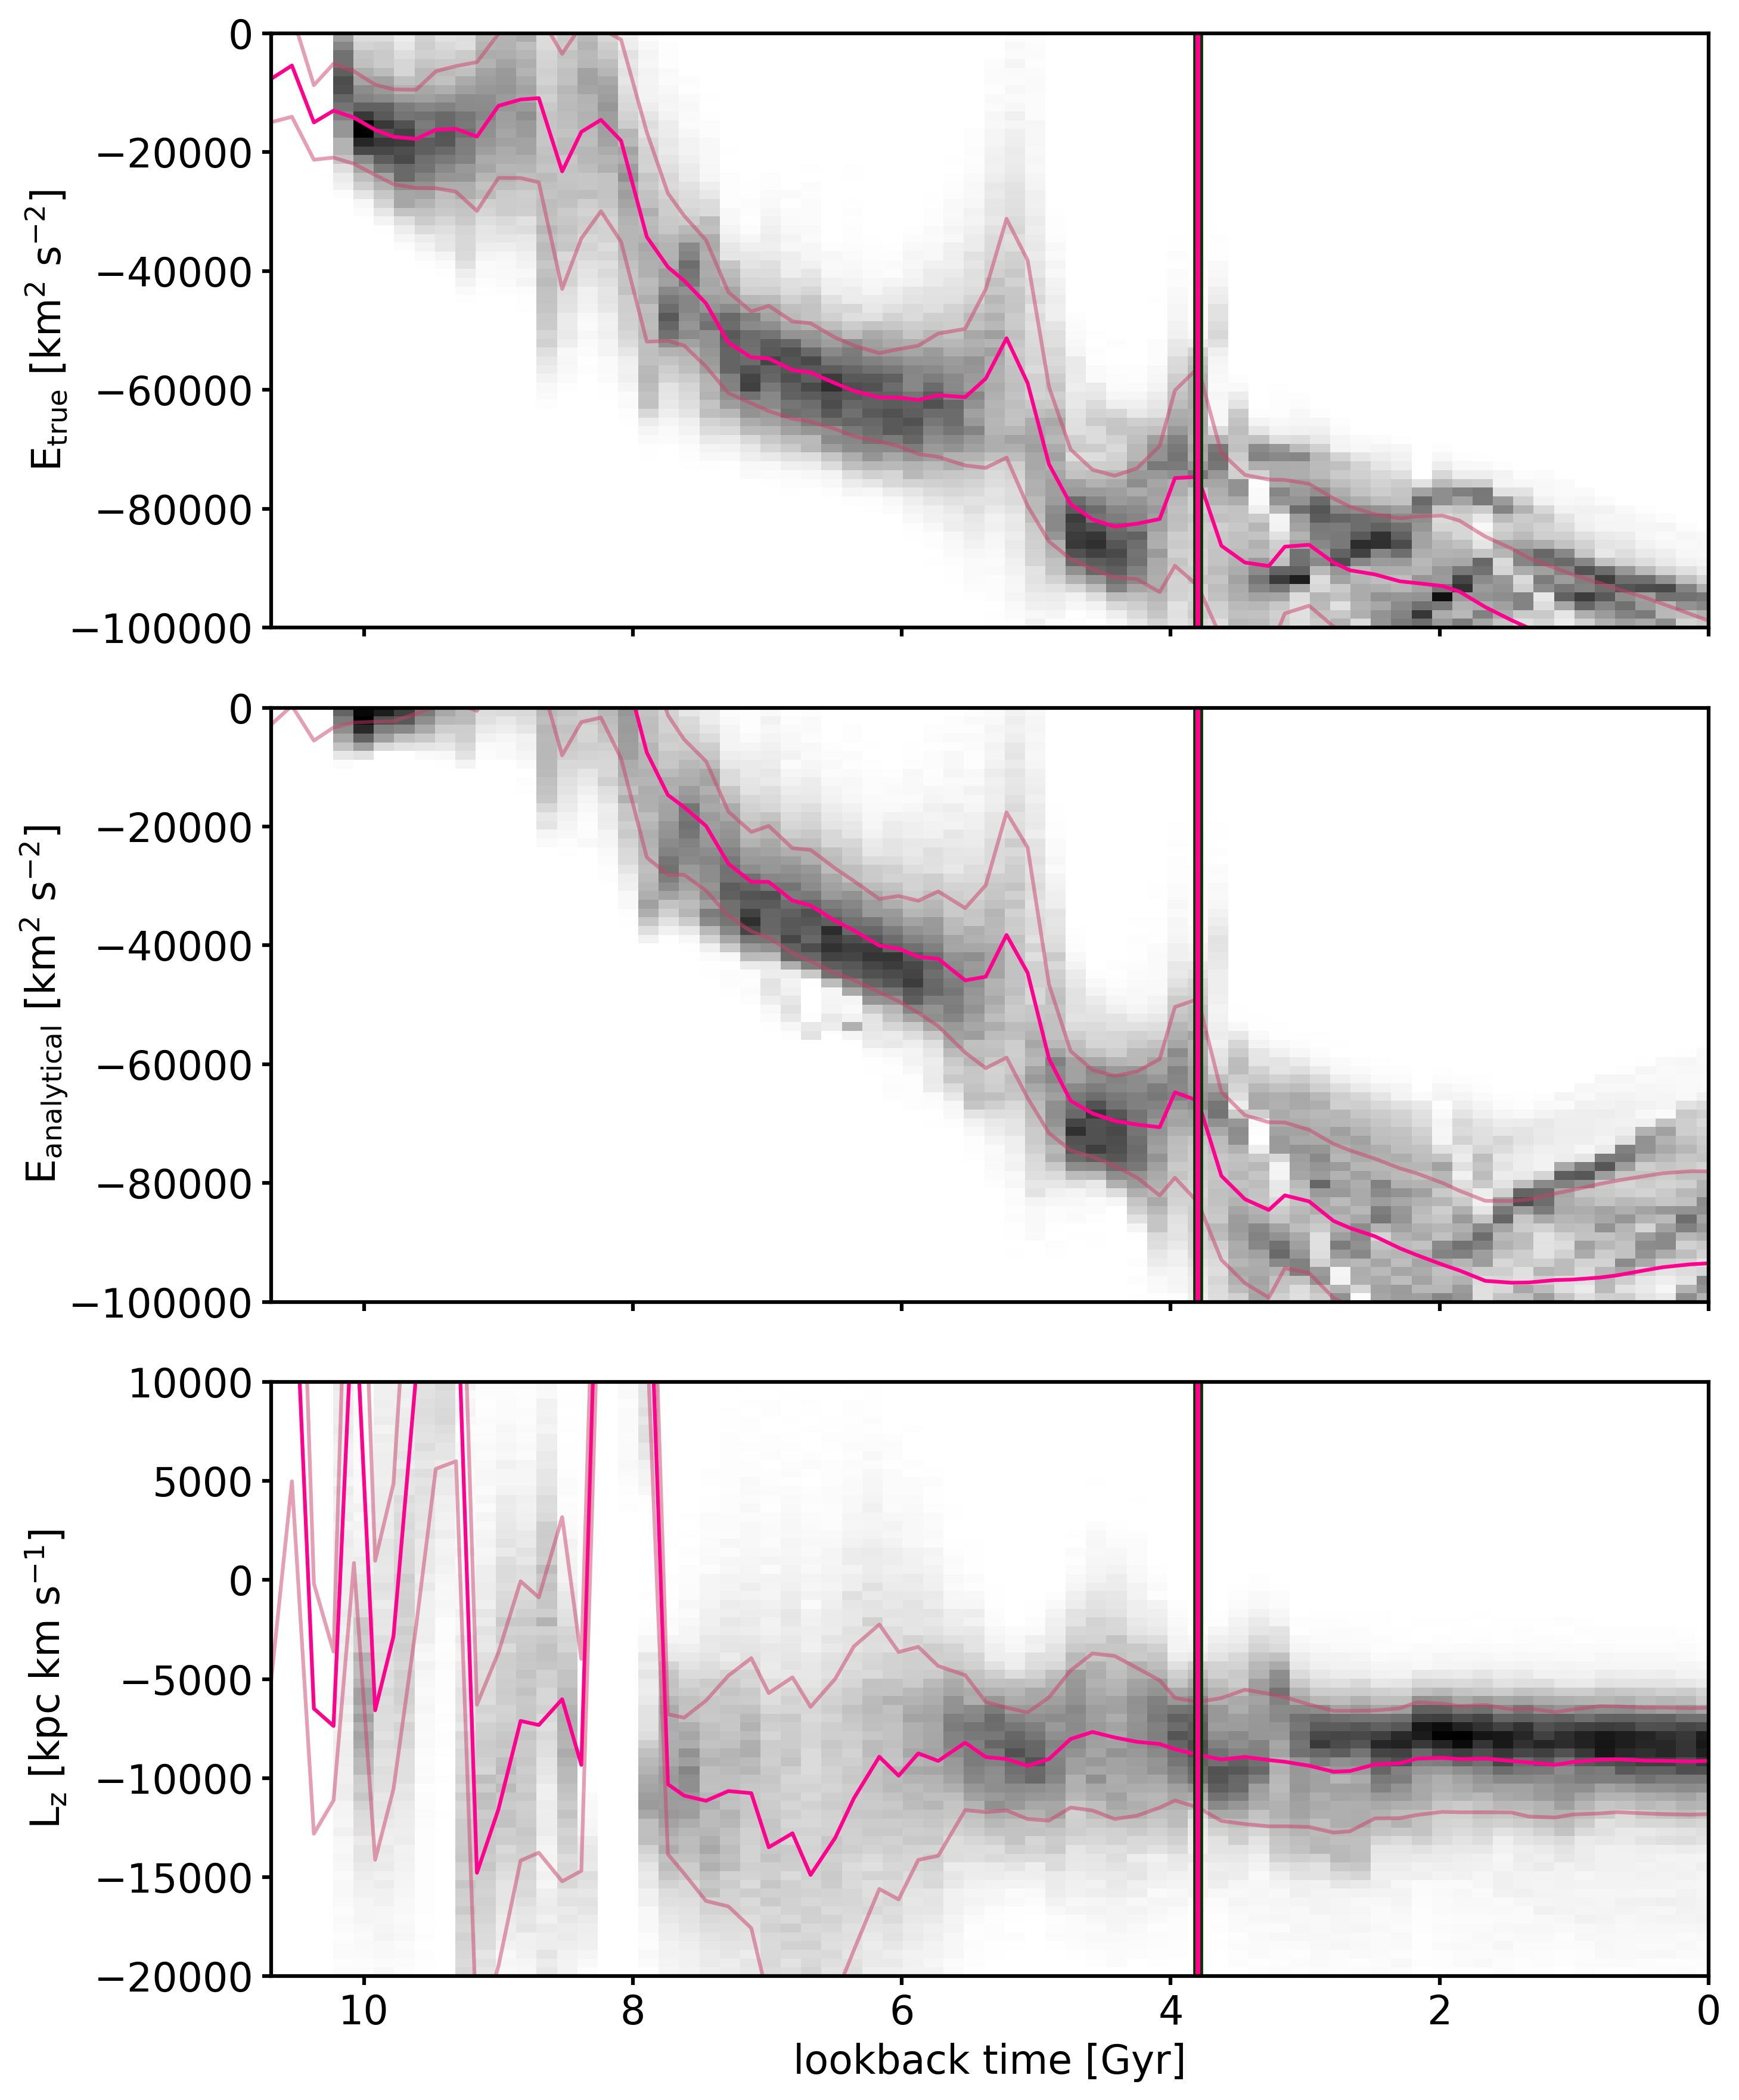
\includegraphics[width=\textwidth]{plots/Dynamics/prog2/energy_time_evolution_hist_mean.png}
	\caption{Time evolution of the energy of the particles of prog2. \textit{Upper panel}: The true energy, which the particles have according to their kinetic energy and their potential value. \textit{Middle panel}: Energy calculated in the best fit potential. \textit{Lower panel}: Angular momentum.\textcolor{red}{update with new selected GCs coming}}\label{fig:energy_time_evolution_prog2}
\end{figure}

We show the energy evolution in Figure \ref{fig:energy_time_evolution_prog2}. Here it again becomes obvious, that the potential fit could be better since the model overestimates the energy by a few \SI{1000}{km^{2}.s^{-2}}. The overall trend is still similar. As the \ac{DG} spirals in it falls deeper into the potential well. This trend continues even after the merger so. Therefore it still gains energy which makes it even less constant than the actions. We find the same trend for prog3 and prog4. 
\\\\This gives another evidence that within our goal to evaluate the galaxy in an analytic axisymmetric form we do not have problems with our assumptions but it seems that the simulation is just too complex to model it that simple.

\iffalse
\begin{figure}
\captionsetup{format=plain}
    \centering
	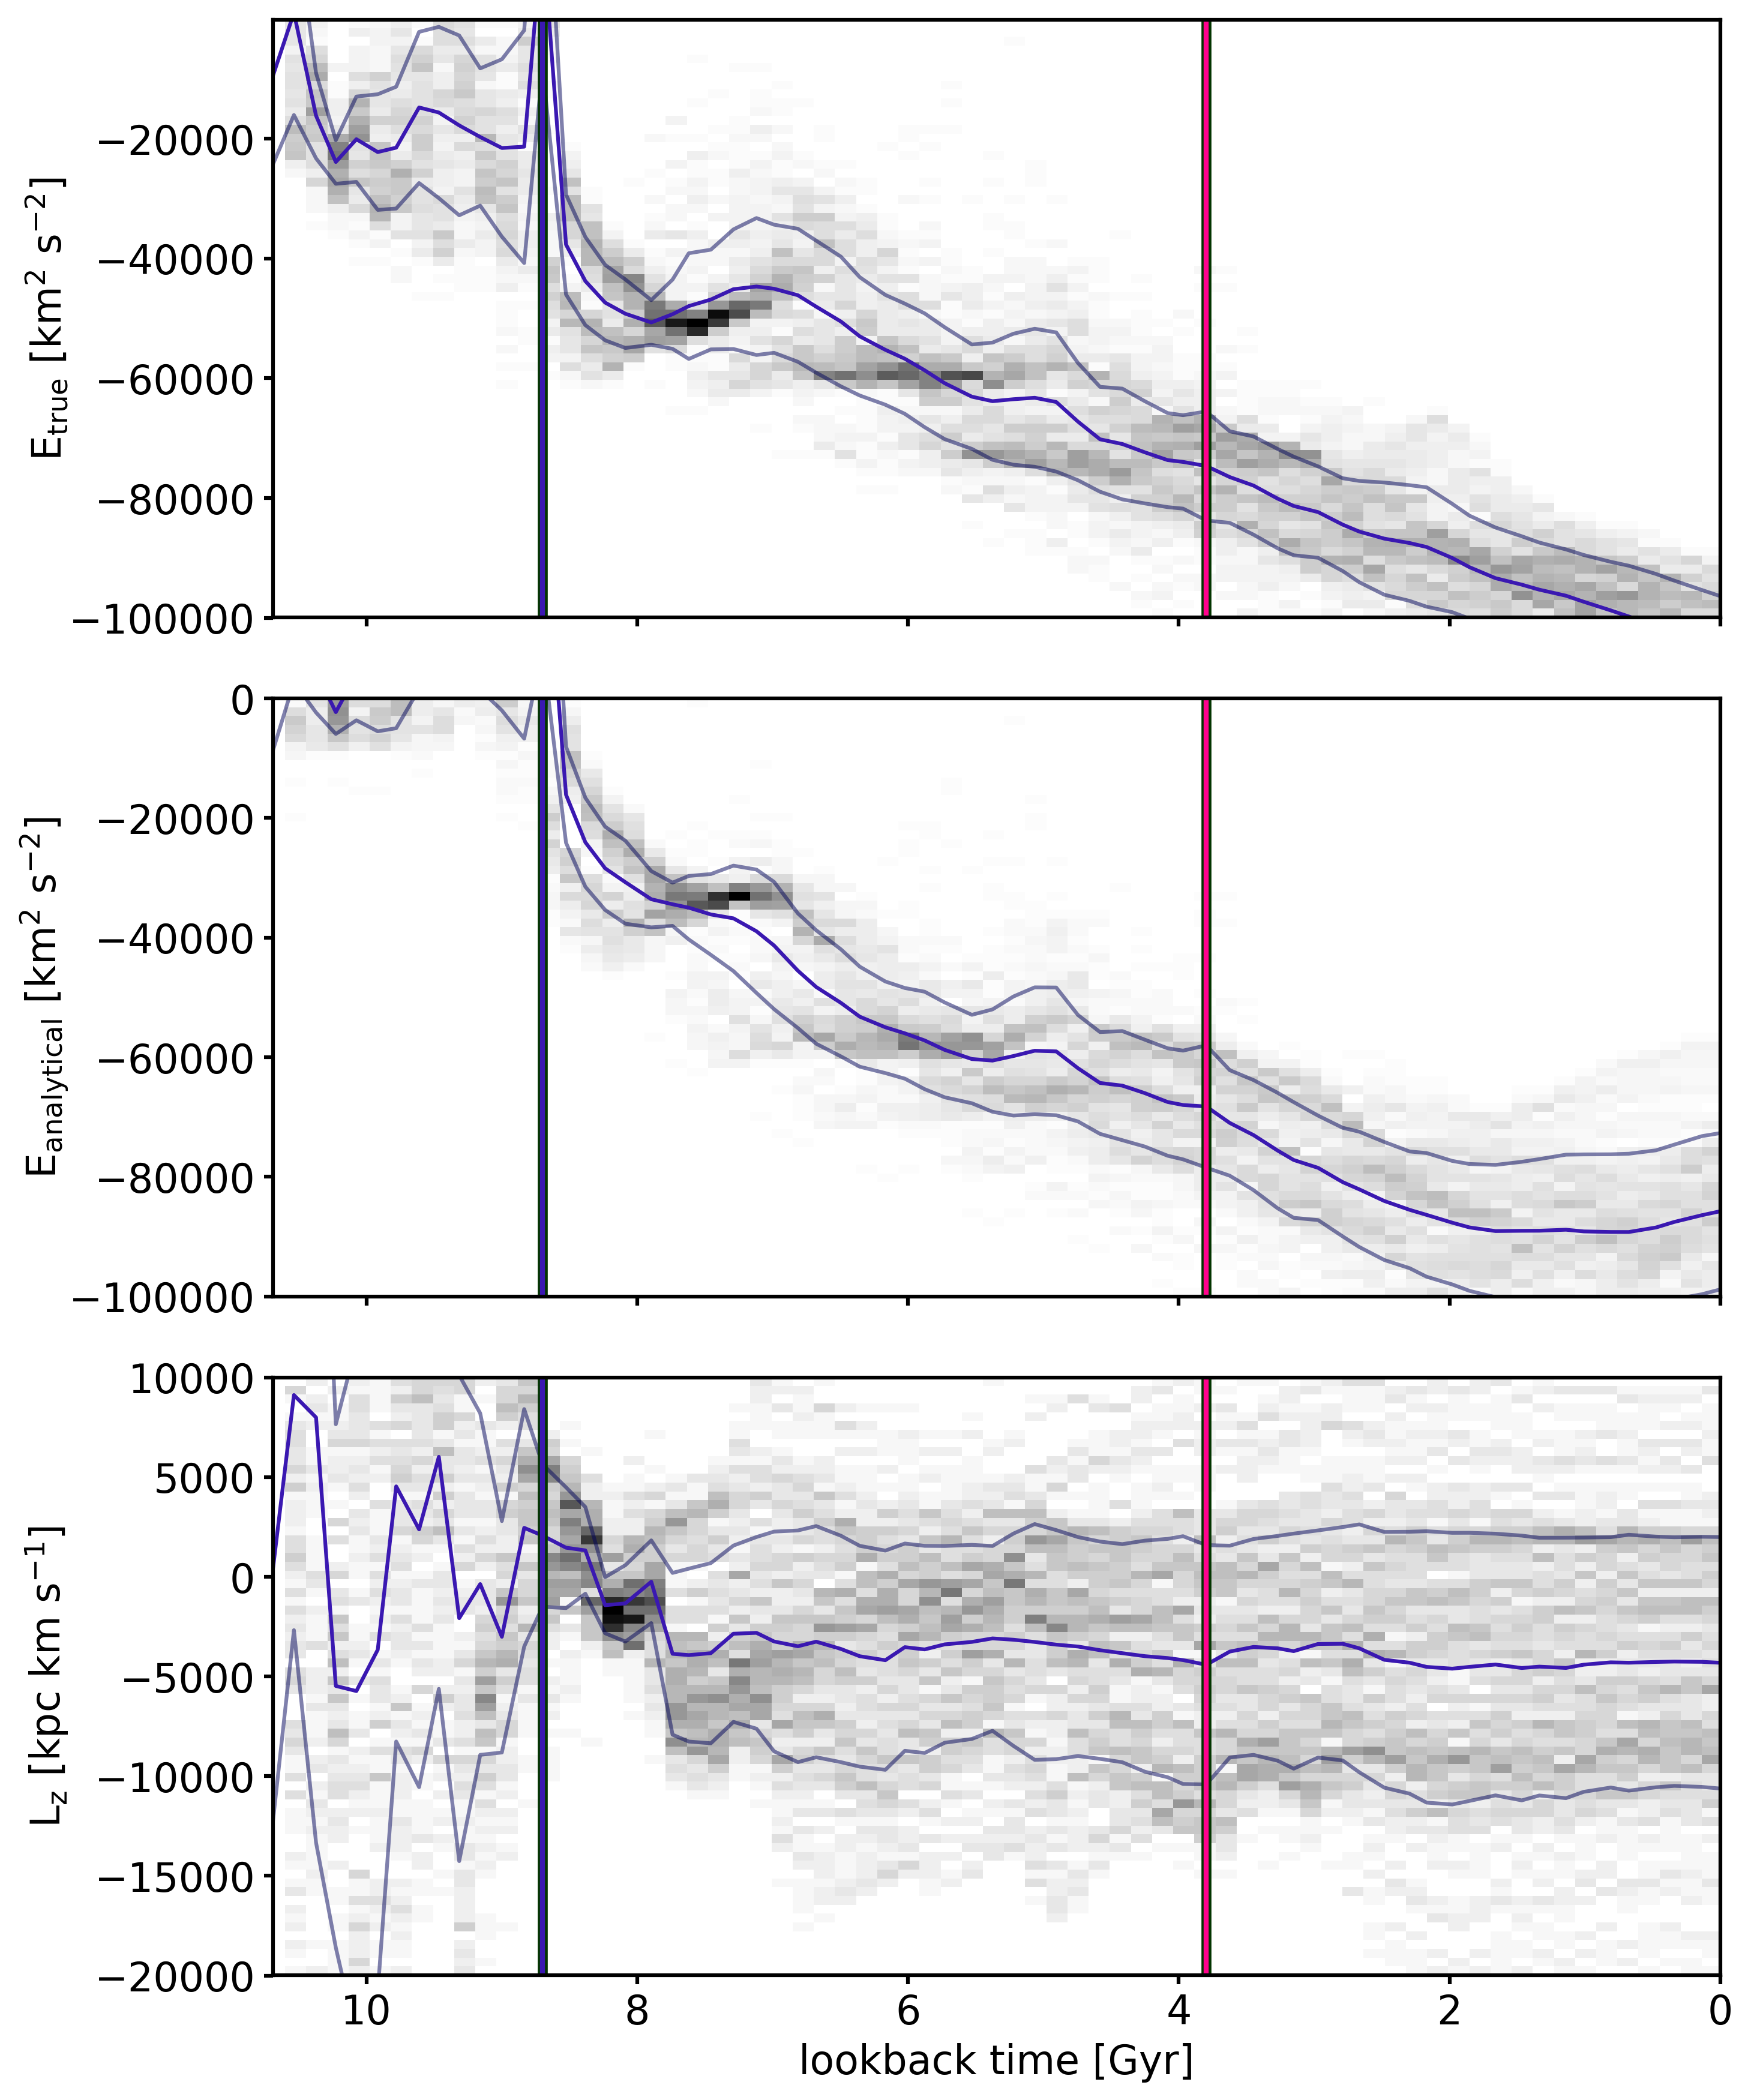
\includegraphics[width=\textwidth]{plots/Dynamics/prog3/energy_time_evolution_hist_mean.png}
    \caption{Same as \ref{fig:energy_time_evolution_prog2} but for prog3. }\label{fig:energy_time_evolution_prog3}
\end{figure}

\begin{figure}[htbp]
\captionsetup{format=plain}
    \centering
	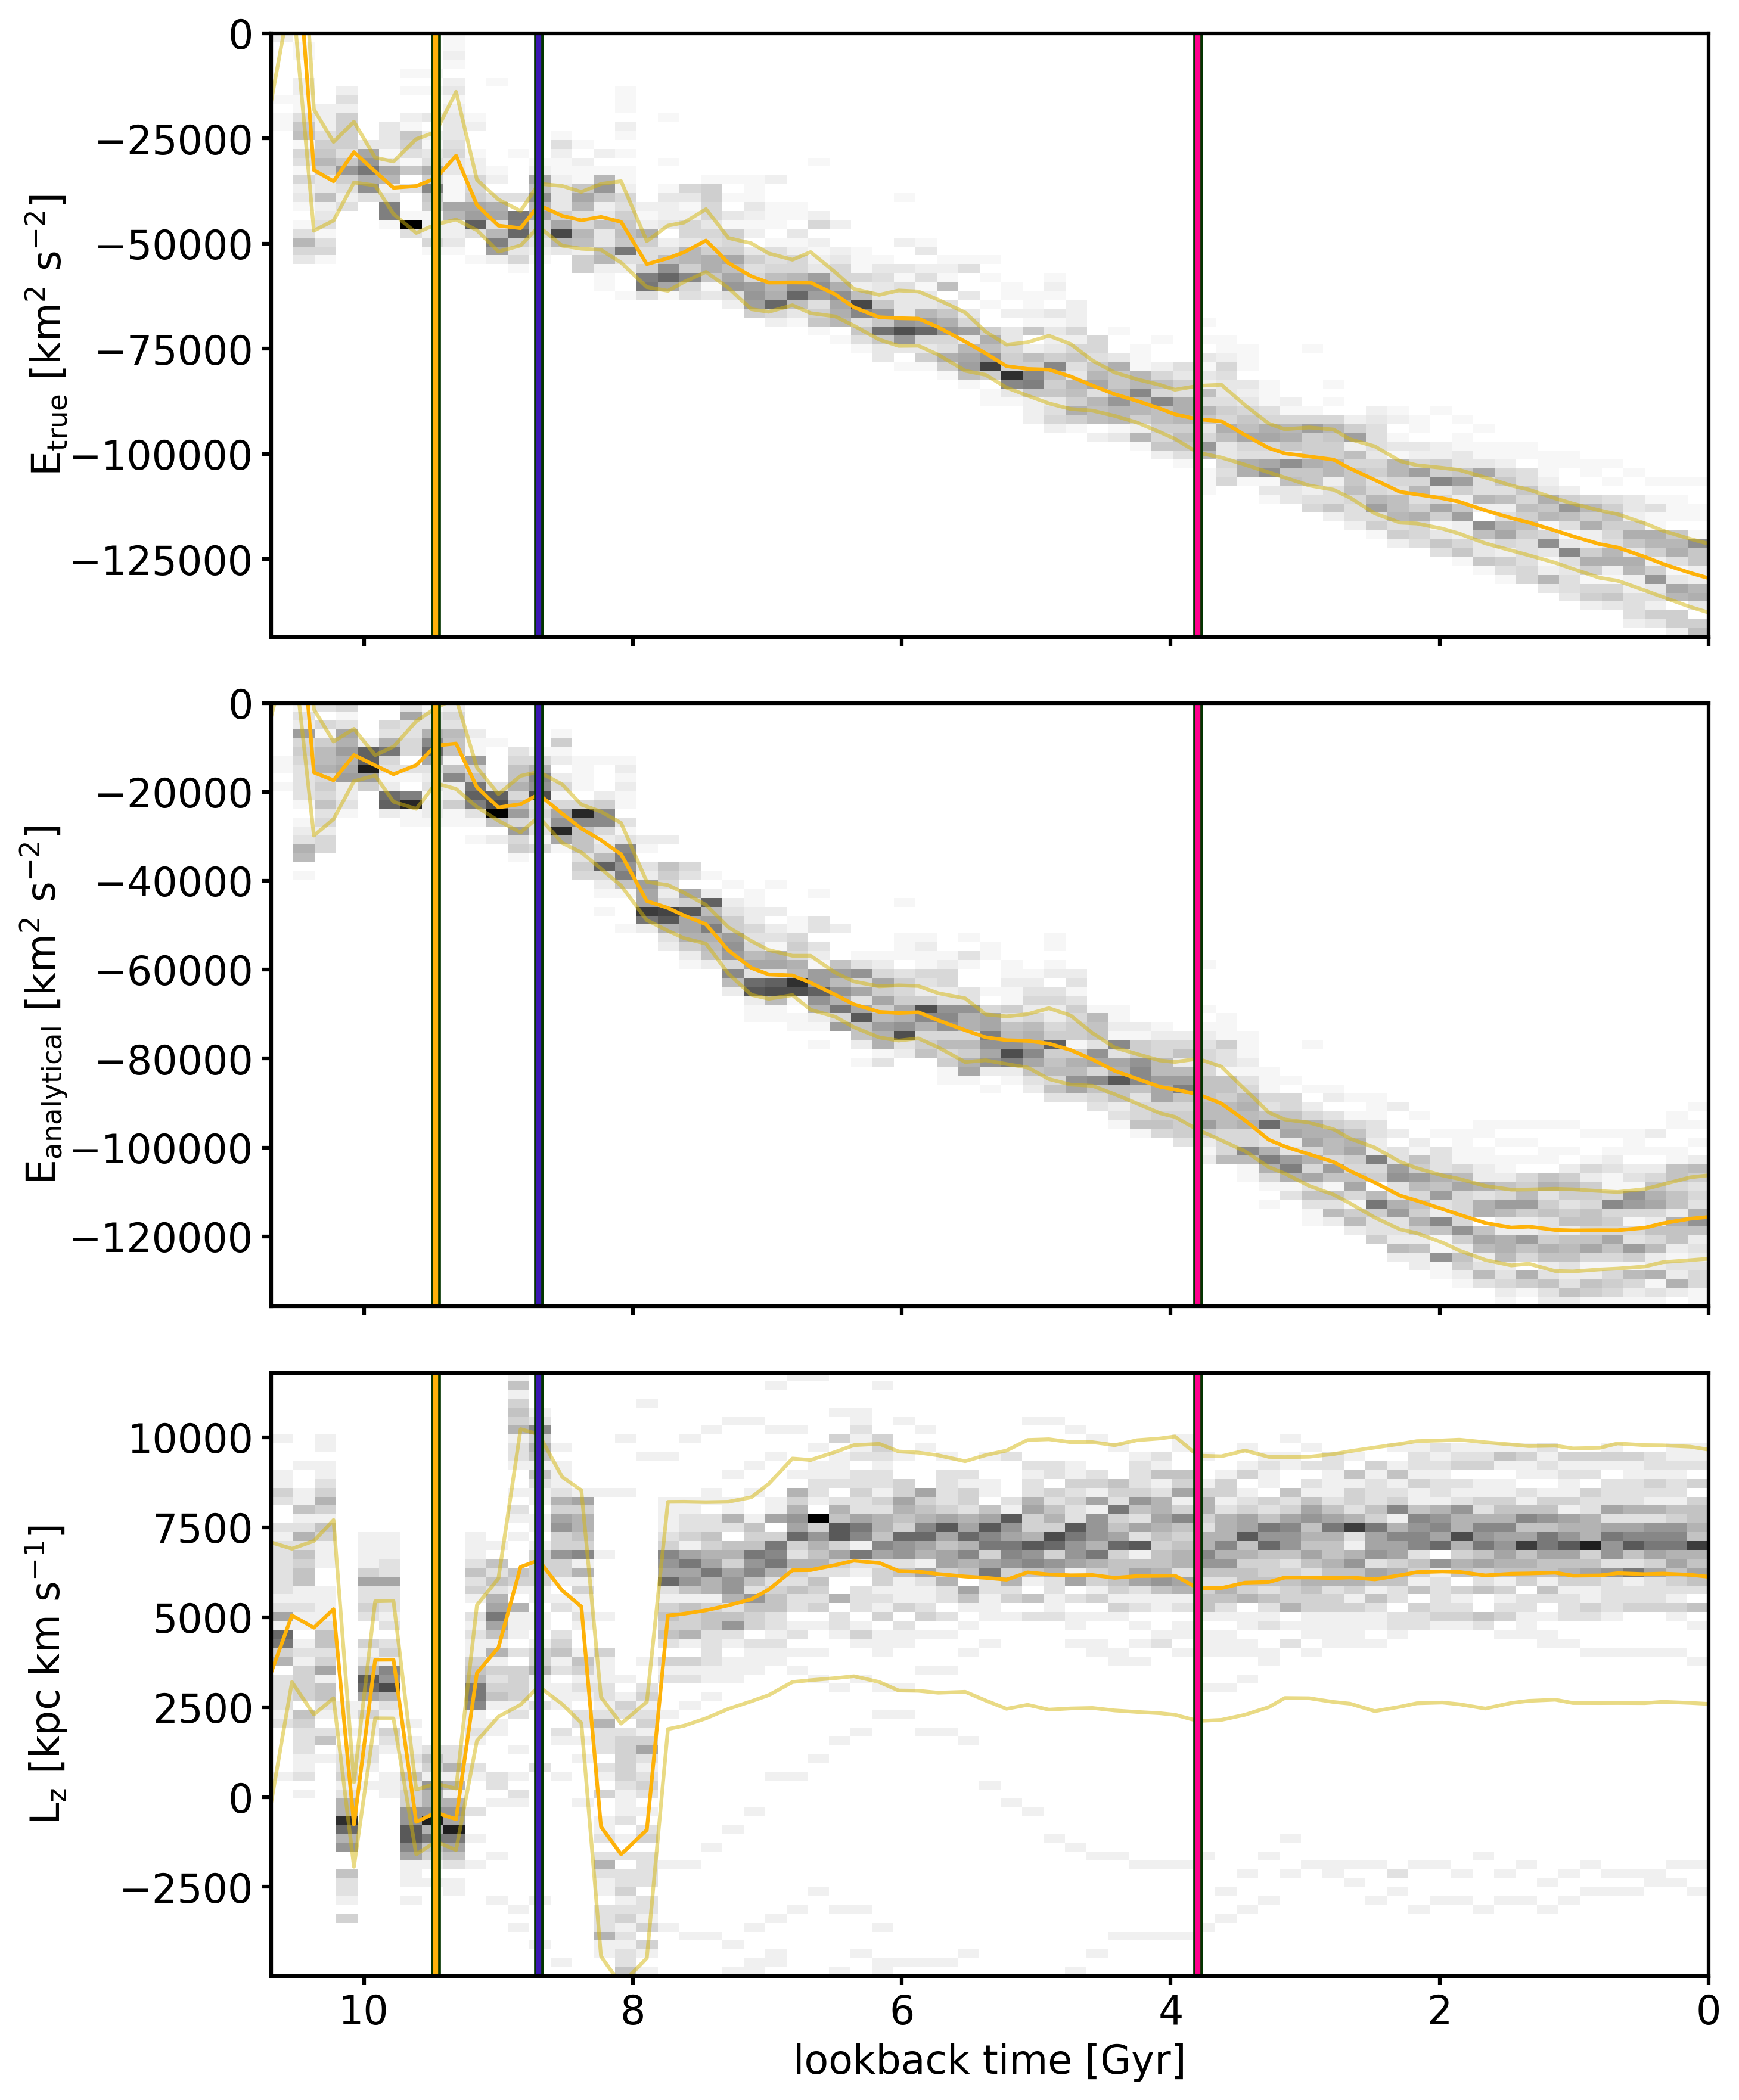
\includegraphics[width=\textwidth]{plots/Dynamics/prog4/energy_time_evolution_hist_mean.png}
    \caption{ame as \ref{fig:energy_time_evolution_prog2} but for prog4.}\label{fig:energy_time_evolution_prog4}
\end{figure}
\fi

\subsection{Test: evolution of globular clusters on same orbit at $z=0$}\label{subsec:box_GCs}
In Section \ref{subsec:GCs_action_space} we found that the overall \ac{GC} distribution in action space is not very clumped. In Section \ref{subsec:time_evo_actions} we saw a rather constant evolution of the actions but with a large scatter. Now we investigate \acp{GC} which actions are close together in the last snapshot. The selection of these 'box \acp{GC}' is made by taking the mean of each action and find all \acp{GC} within a cube centered on the means with a gradually increasing side length. For prog2, we want to look at a larger sample of 20 particles. To have 20 particles in this cube required a side length of \SI{650}{kpc.km.s^{-1}}. Since we have fewer particles accreted from prog3 and prog4, they needed bigger side lengths and therefore the orbits of their box particles are a priori not as close.  

\begin{figure}[htbp]
\captionsetup{format=plain}
    \centering
    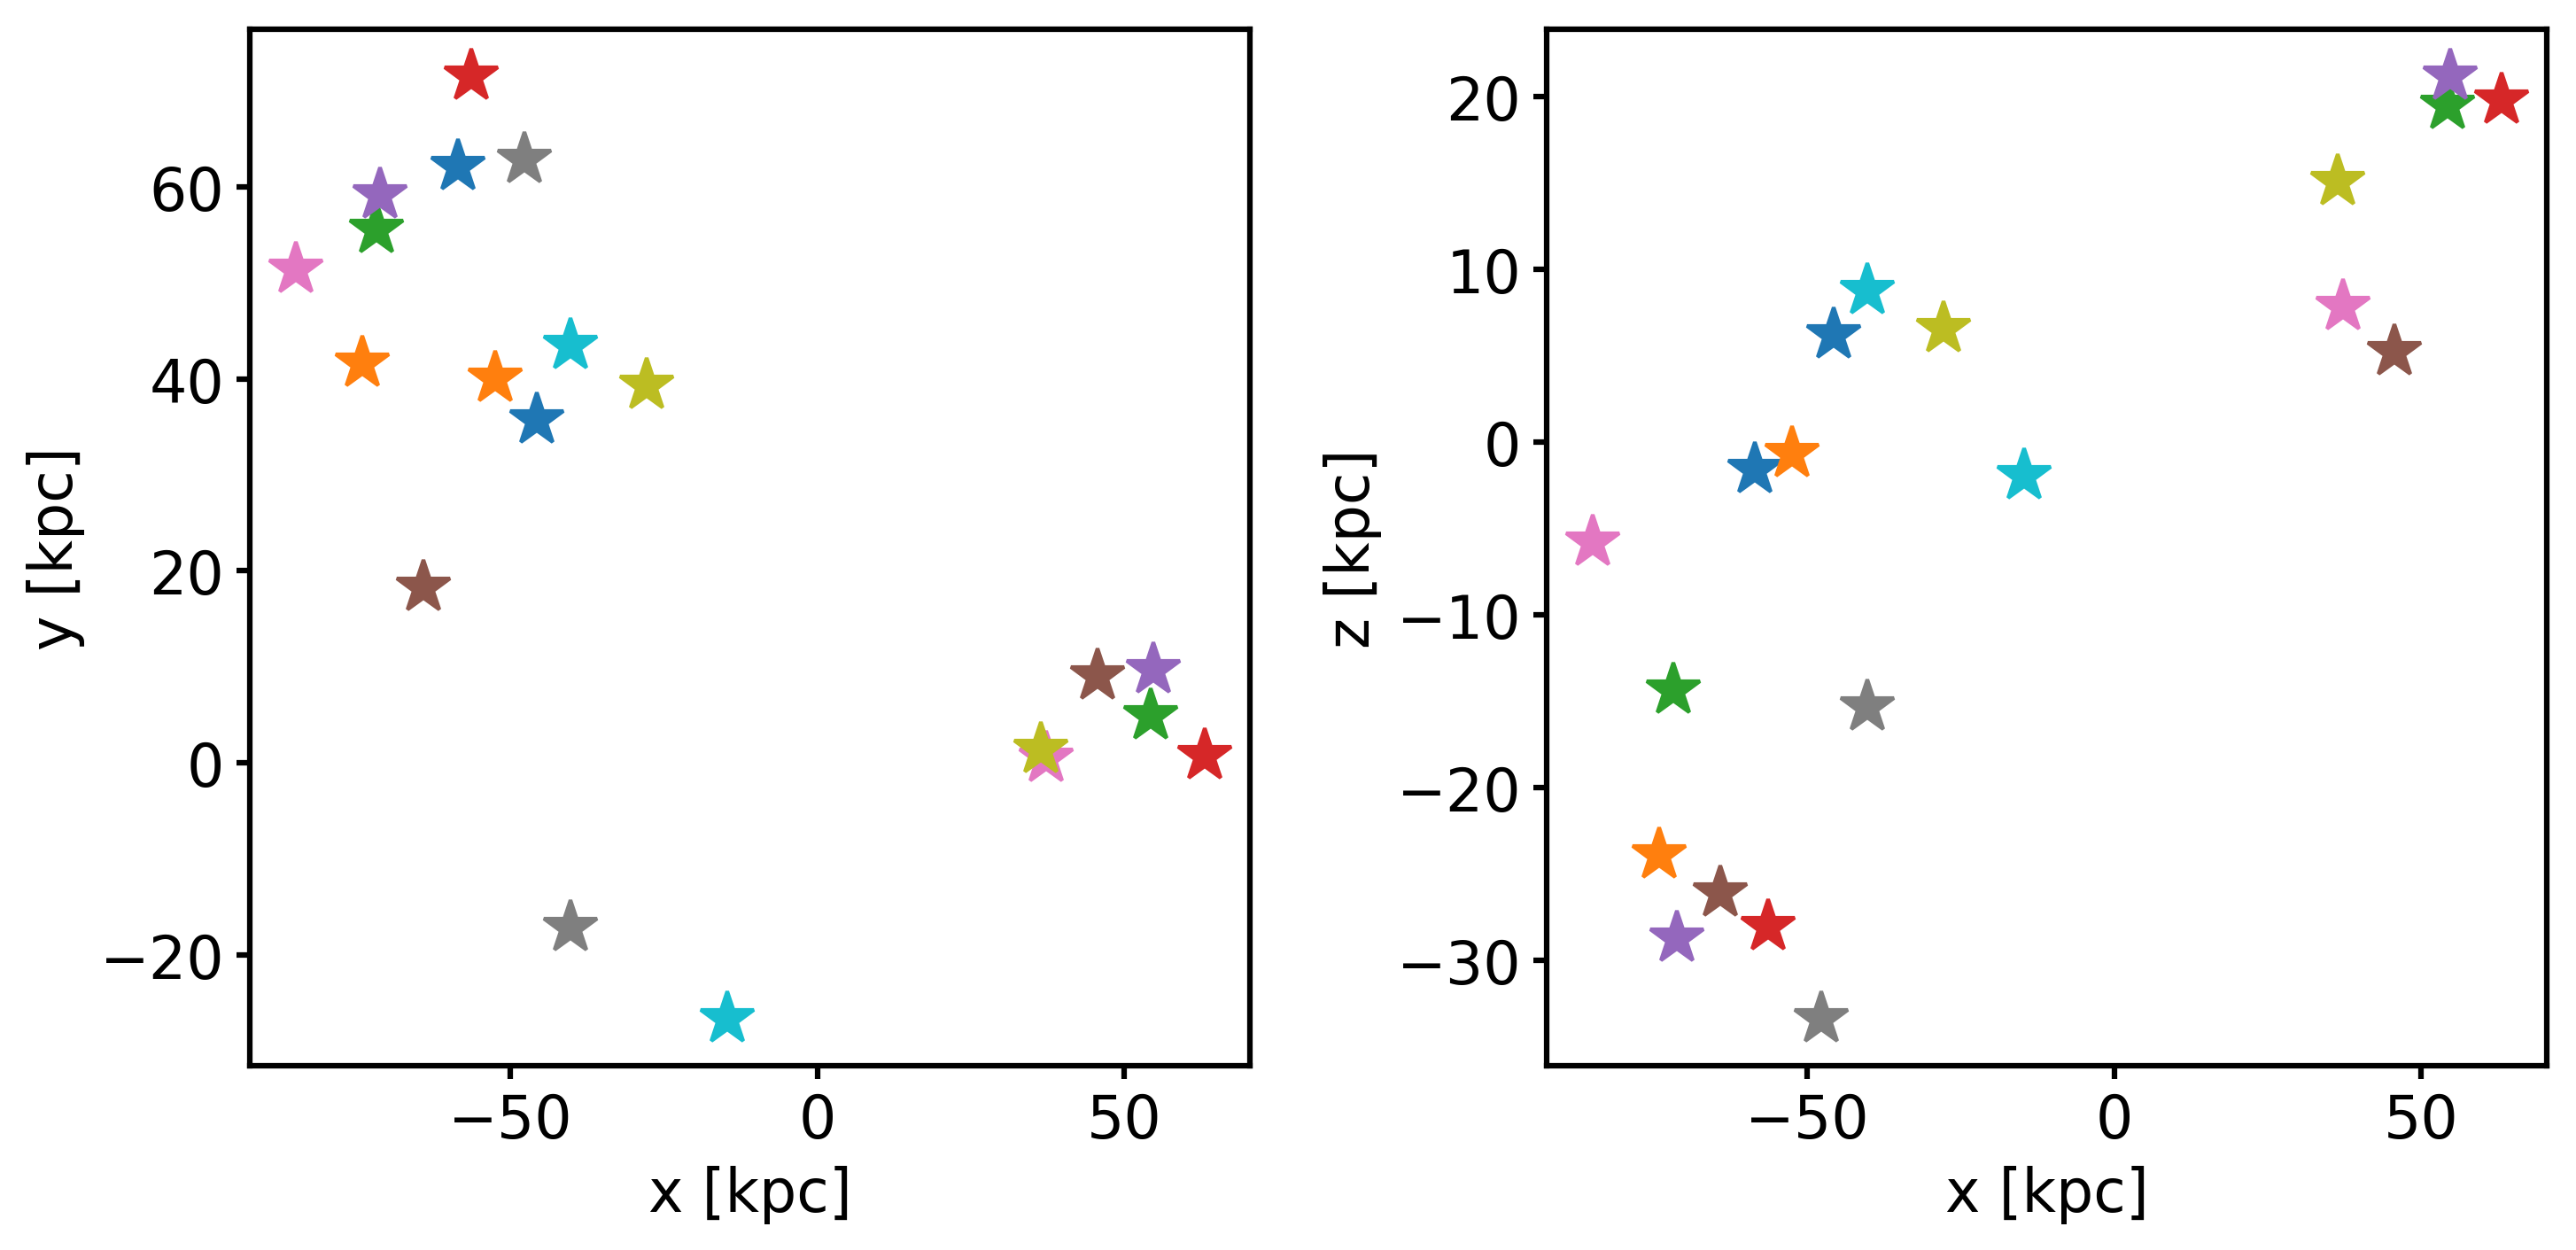
\includegraphics[width=0.9\textwidth]{plots/Dynamics/dist/progenitor2_box_distribution.png}
    \caption{Spatial distribution of selected box particles. \textcolor{red}{update with new selected GCs and therefore new boxcoming}}
    \label{fig:box_GCs_distr}
\end{figure}

Their spatial distribution is presented in Figure \ref{fig:box_GCs_distr}. There is a small clustering around $x = \SI{50}{kpc}$ but all other selected GCs are well distributed in phase-space. 


\begin{figure}[htbp]
\captionsetup{format=plain}
    \centering
	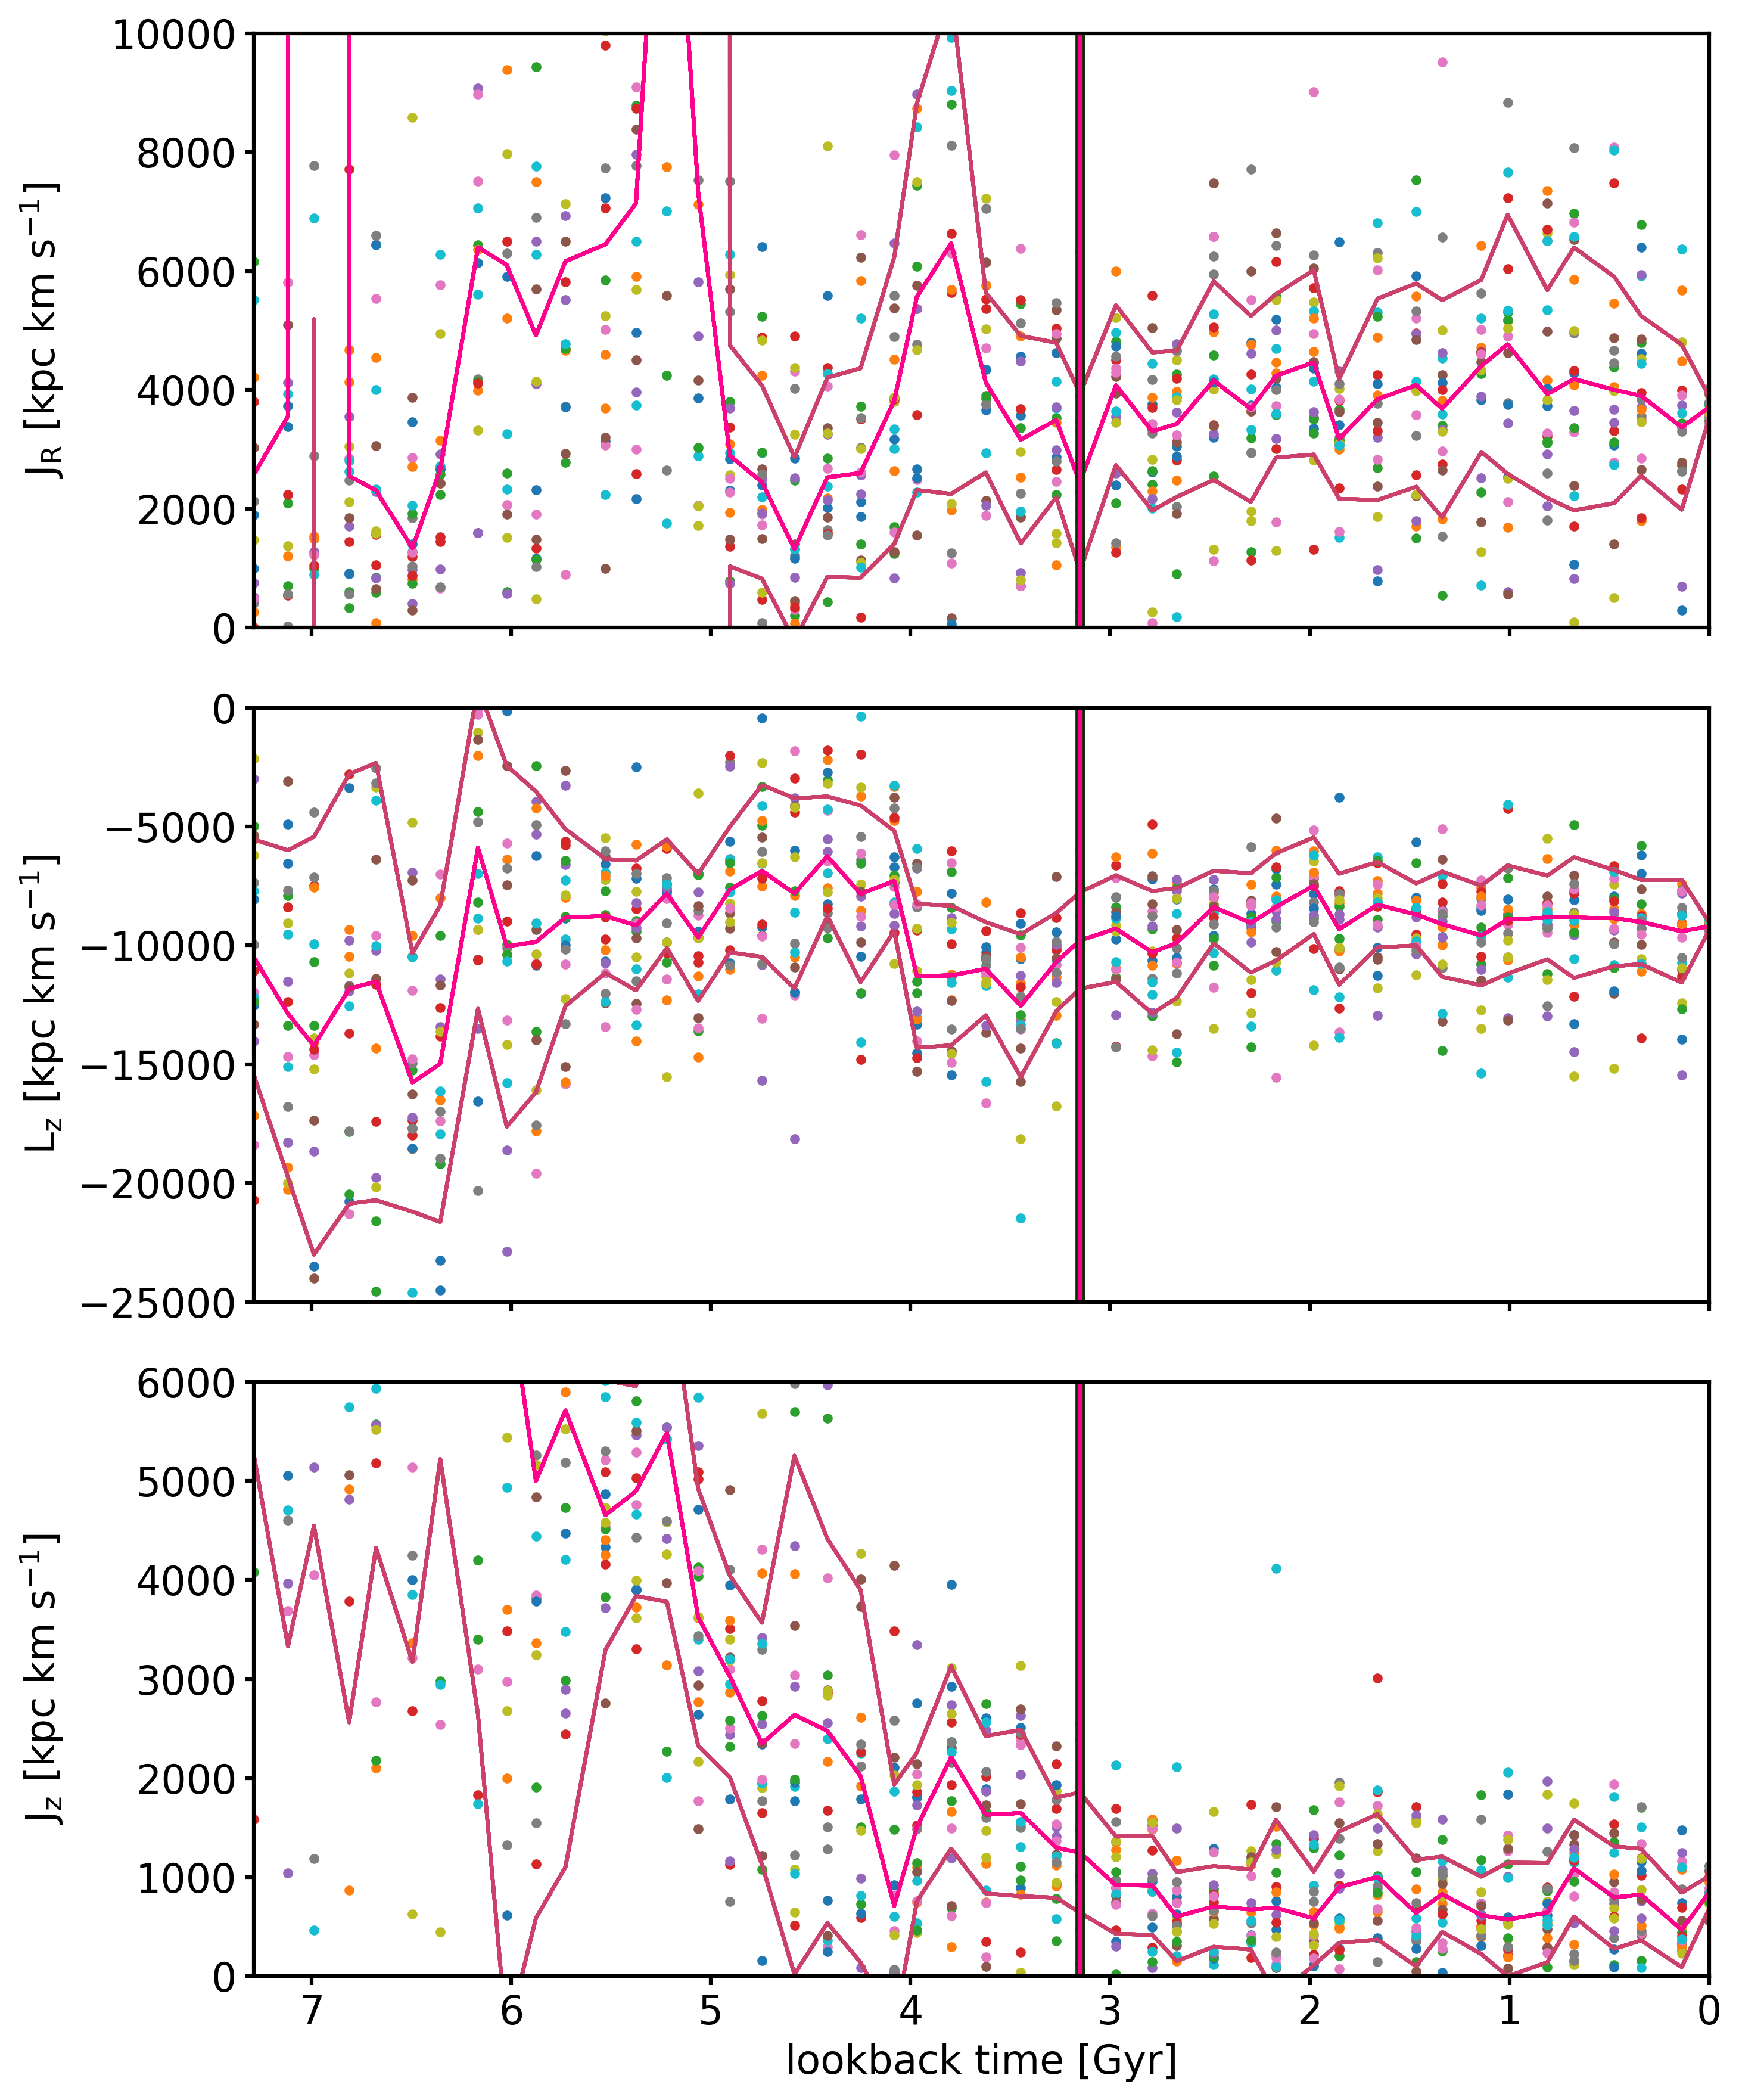
\includegraphics[width=\textwidth]{plots/Dynamics/prog2/action_time_evolution_box_hist_mean_prog2.png}

	\caption{Action time evolution of 17 particles of prog2 which are found to be on similar orbits in the $z=0$ snapshot. \textcolor{red}{update with new selected GCs and therefore new boxcoming} }\label{fig:actions_box_time_evolution_prog2}
\end{figure}
In Figure \ref{fig:actions_box_time_evolution_prog2}, we plot the evolution of these actions. At the last snapshot, we see how close they are in all three actions. But already one snapshot before, they spread out widely and do not have any connection. Going back in time, the spread approximately stays constant. So even though we find similar orbit parameters at the very end, they do not evolve similarly. If we found \acp{GC} clumped together in actions today, they could have a similar evolution and would just be on the same orbit now by chance.

\begin{figure}[htbp]
\captionsetup{format=plain}
    \begin{subfigure}[c]{0.48\textwidth}
    \centering
    	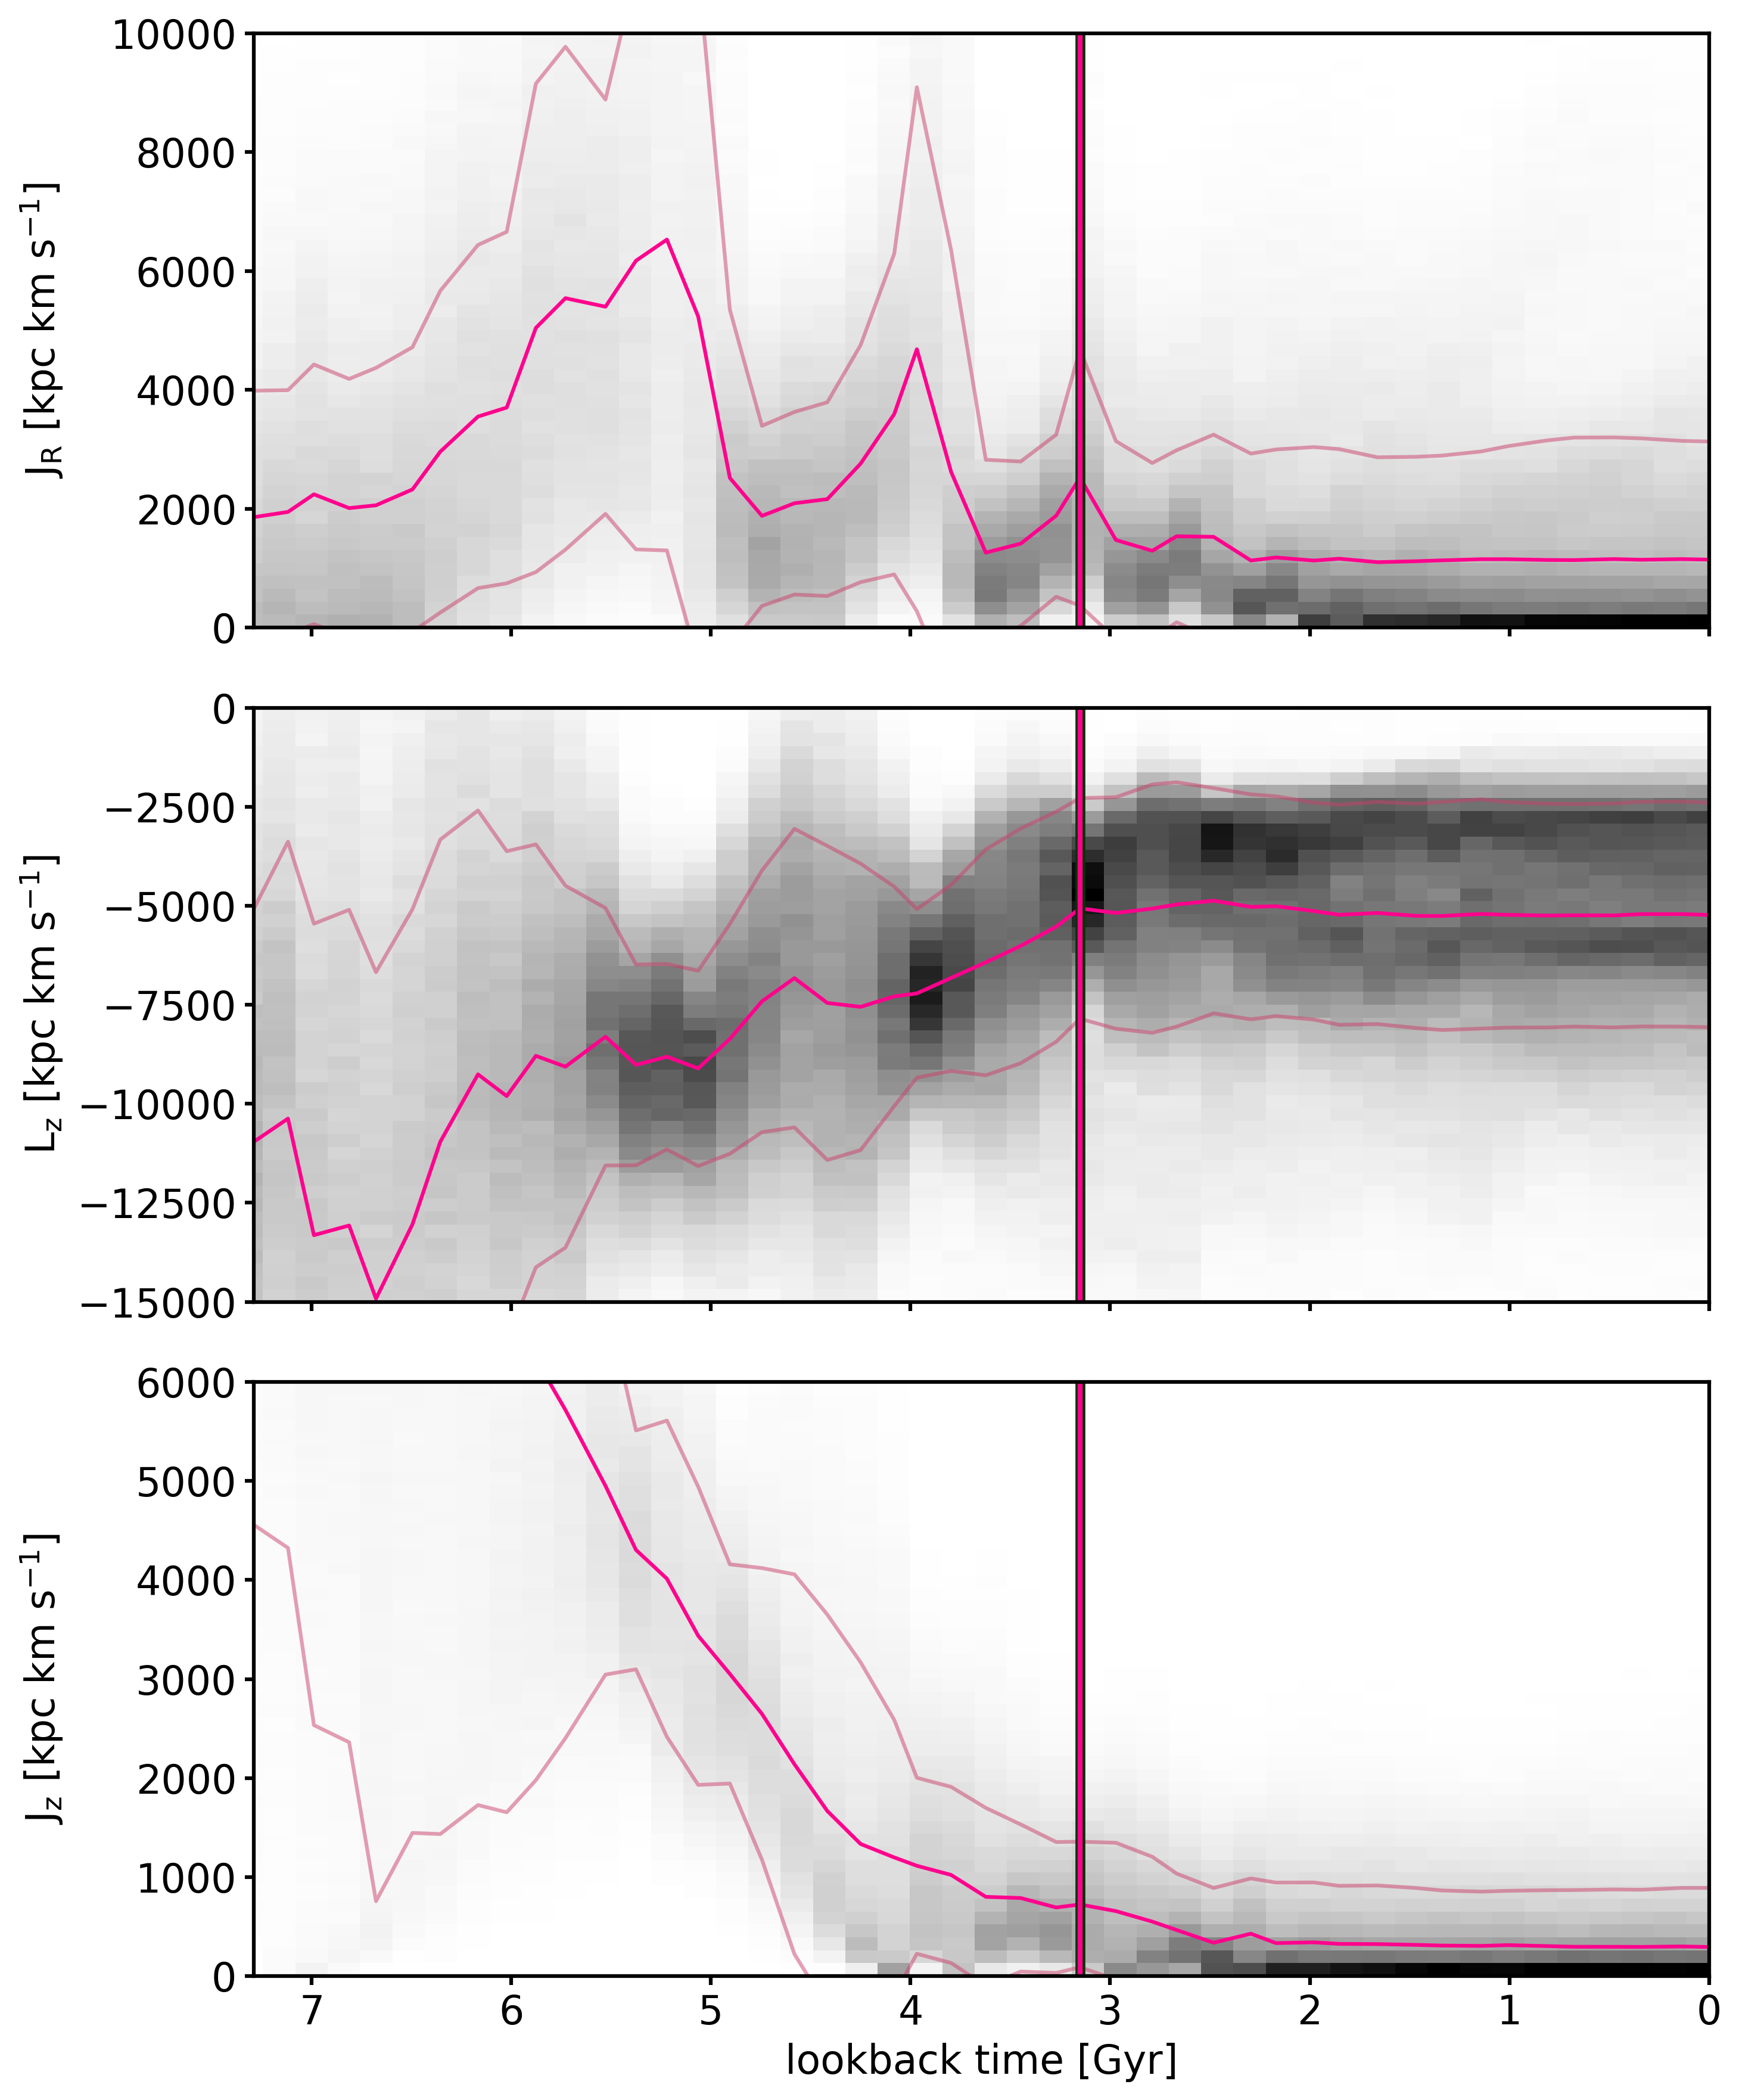
\includegraphics[width=\textwidth]{plots/Dynamics/prog2/action_time_evolution_wodisk_hist_mean.png}
    \end{subfigure}
    ~
    \begin{subfigure}[c]{0.48\textwidth}
    \centering
	    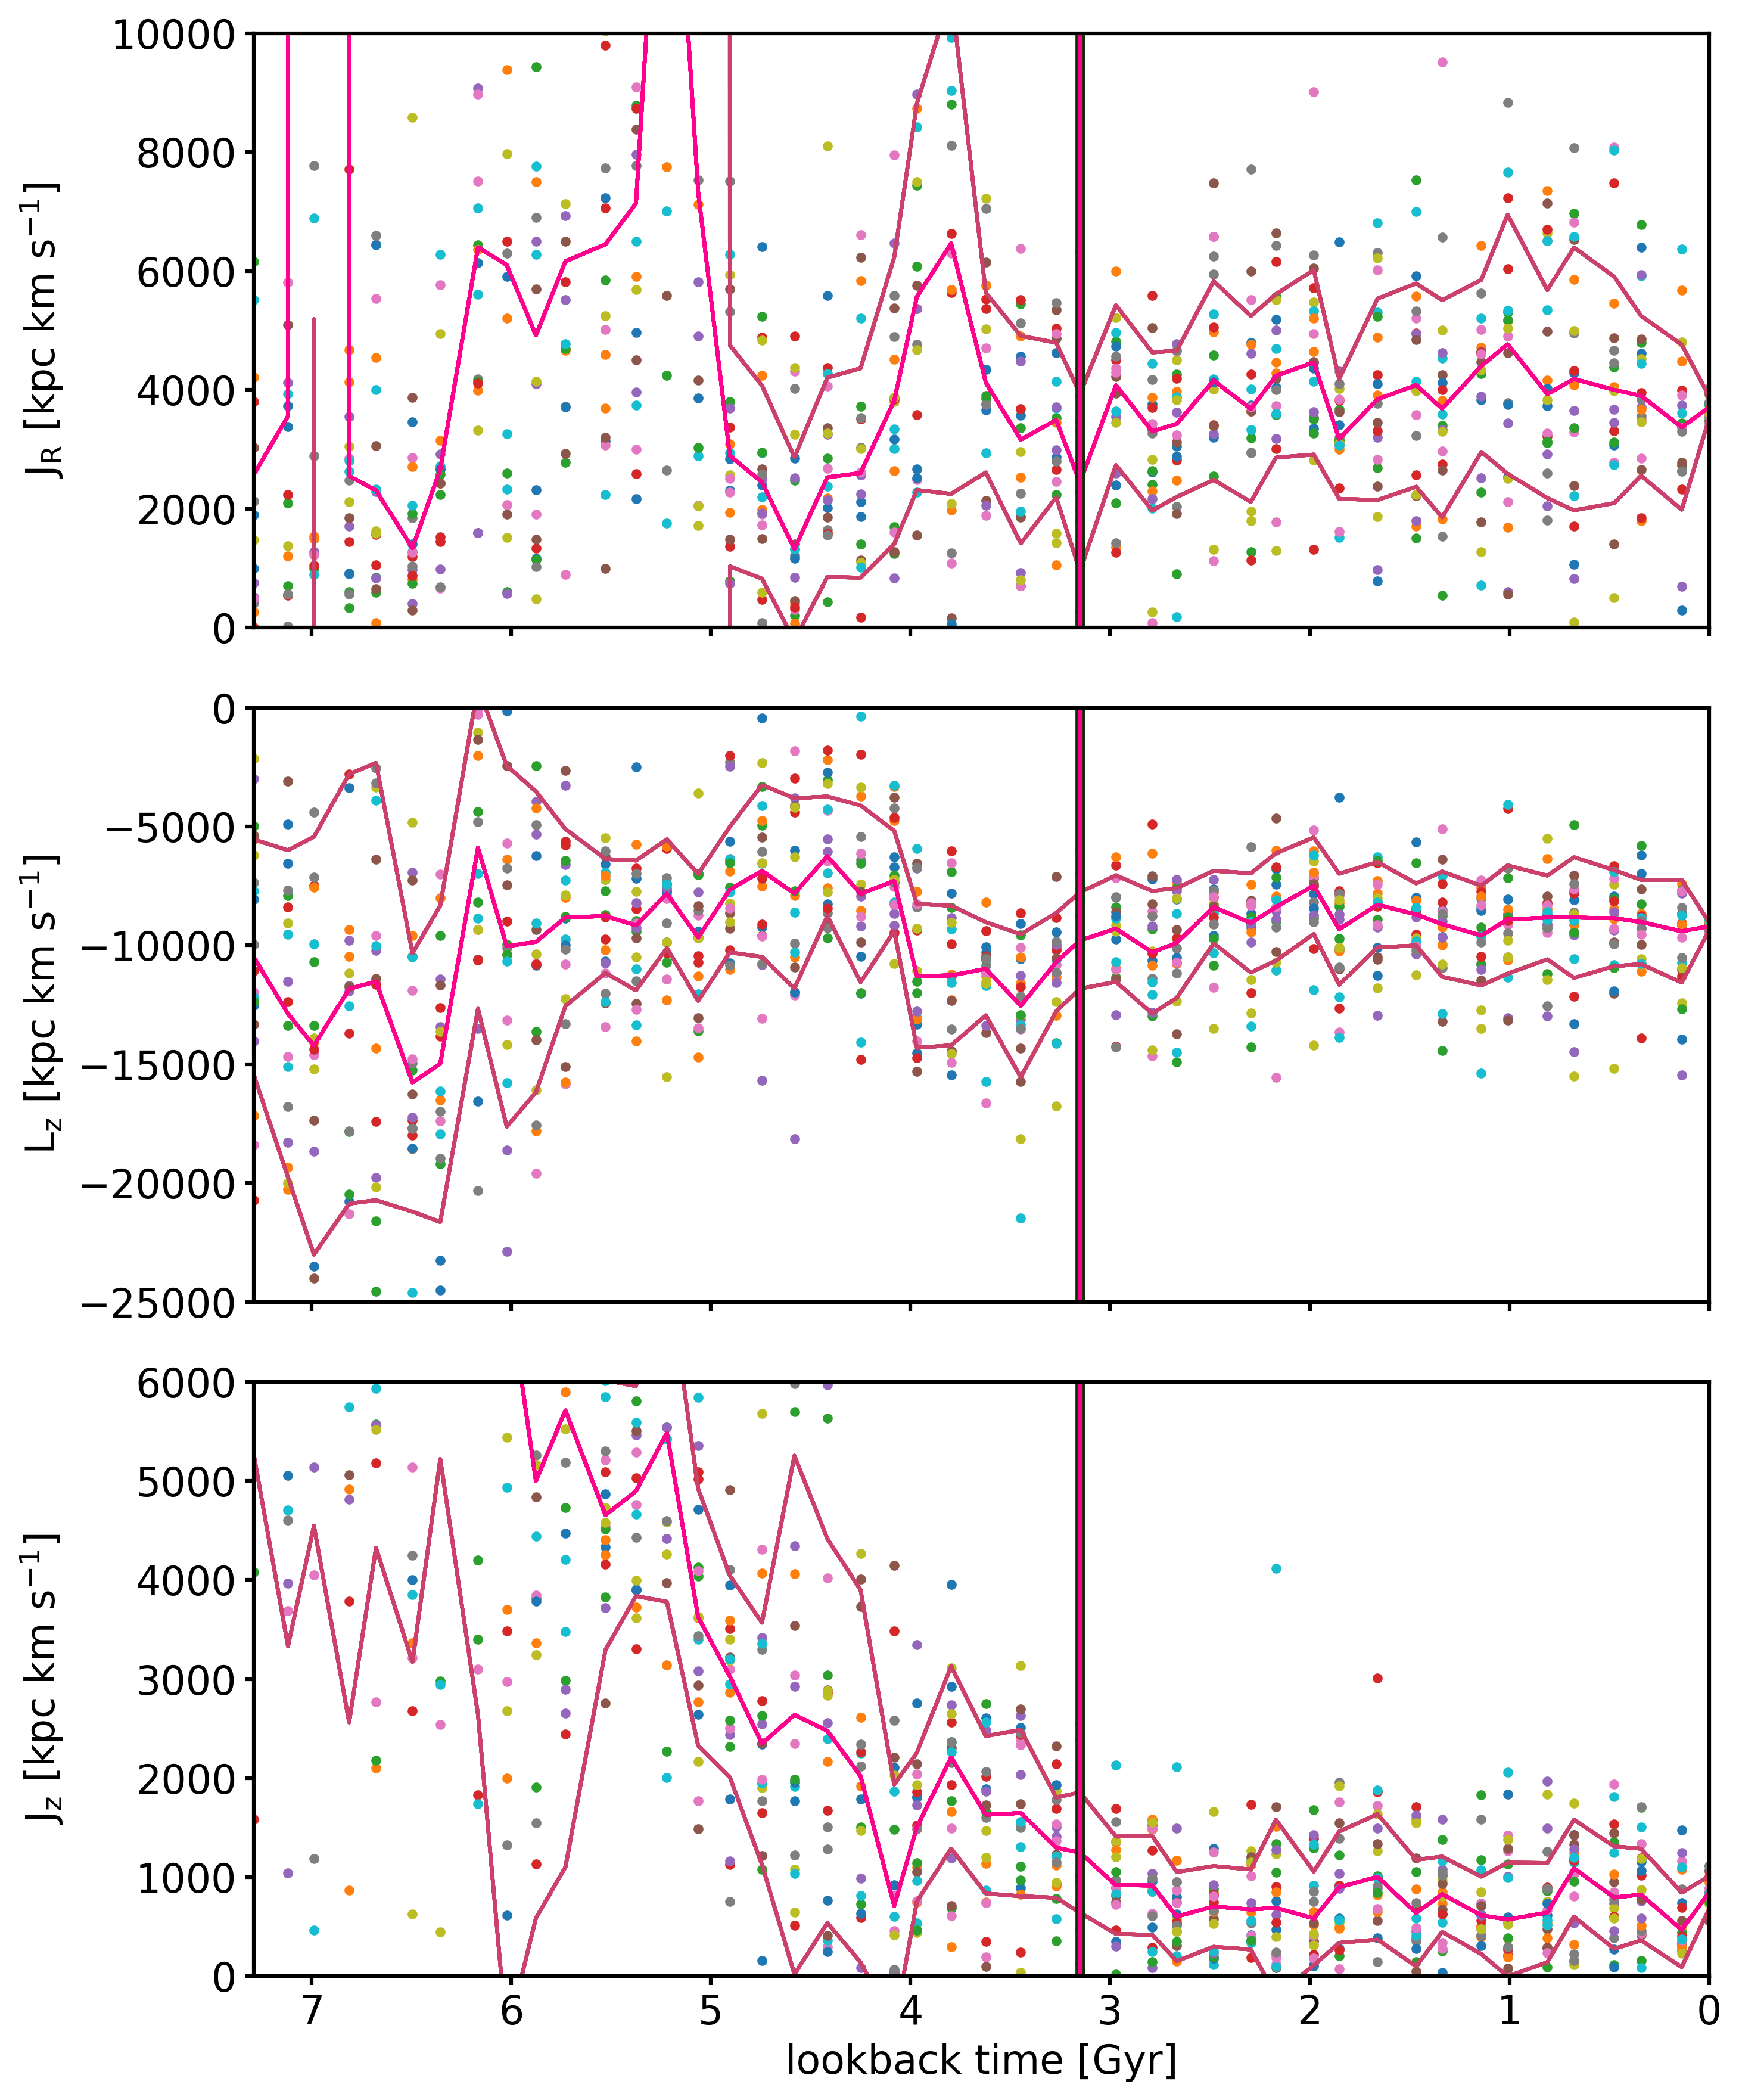
\includegraphics[width=\textwidth]{plots/Dynamics/prog2/action_time_evolution_box_hist_mean_prog2.png}
    \end{subfigure}
    \caption{\textcolor{red}{update with new selected GCs and therefore new boxcoming}}\label{fig:comparison_actions_time_evolution_box_prog2}
\end{figure}
We compare the evolution of the box particles to the evolution of all accreted particles from prog2 in Figure \ref{fig:comparison_actions_time_evolution_box_prog2}. The median and standard deviations evolve around the same values. This is another confirmation that at $z=0$ the box particles ave only by chance similar orbit parameters and evolve within the overall distribution over time. \\\\
We constructed a case in which we find a few \acp{GC} on similar orbits at the current time as we find them in observations. These could be used to constrain the potential by minimizing their spread. Looking at their time evolution leads to the conclusion that they are only on same orbits right now by chance and will have different properties soon again. So even if constraining the potential by minimizing the spread of accreted \acp{GC} in action would work we need to be careful in the selection of these \acp{GC}.
\iffalse
\begin{figure}
\captionsetup{format=plain}
    \centering
	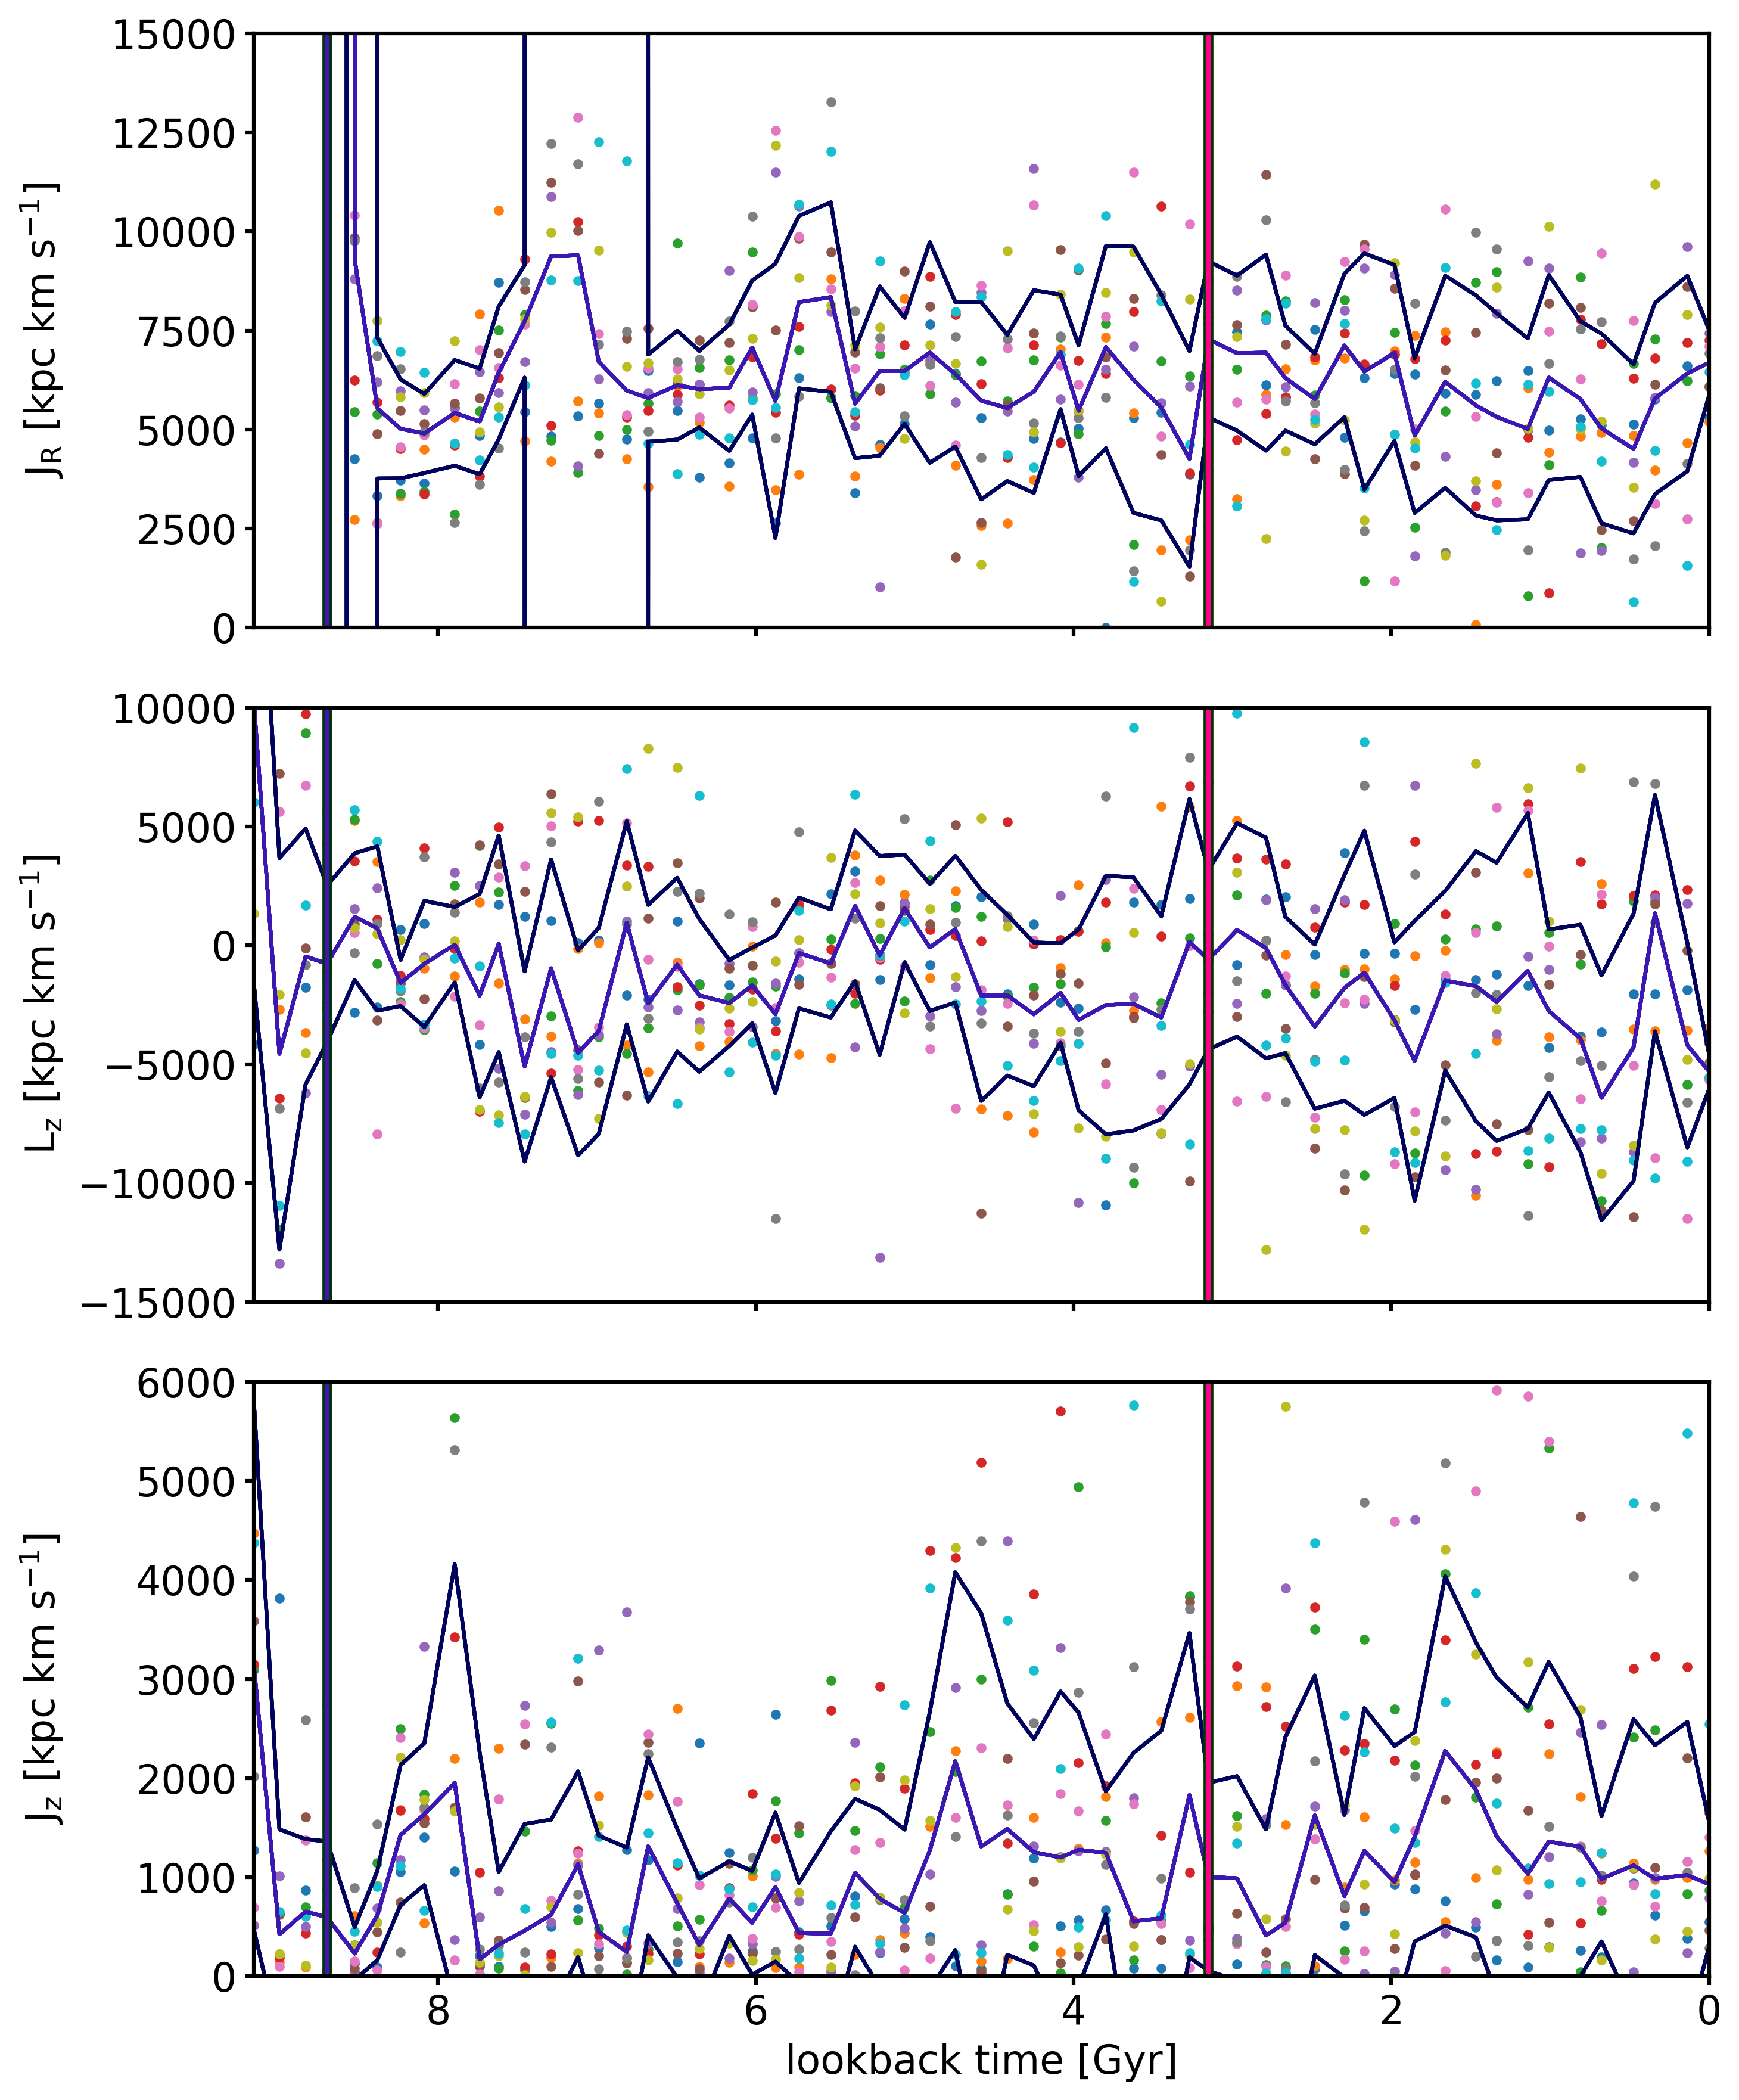
\includegraphics[width=\textwidth]{plots/Dynamics/prog3/action_time_evolution_box_hist_mean_prog3.png}
    \caption{Action time evolution of xx particles of prog3 which are found to be on similar orbits in the $z=0$ snapshot.}\label{fig:actions_box_time_evolution_prog3}
\end{figure}

\begin{figure}[htbp]
\captionsetup{format=plain}
    \centering
	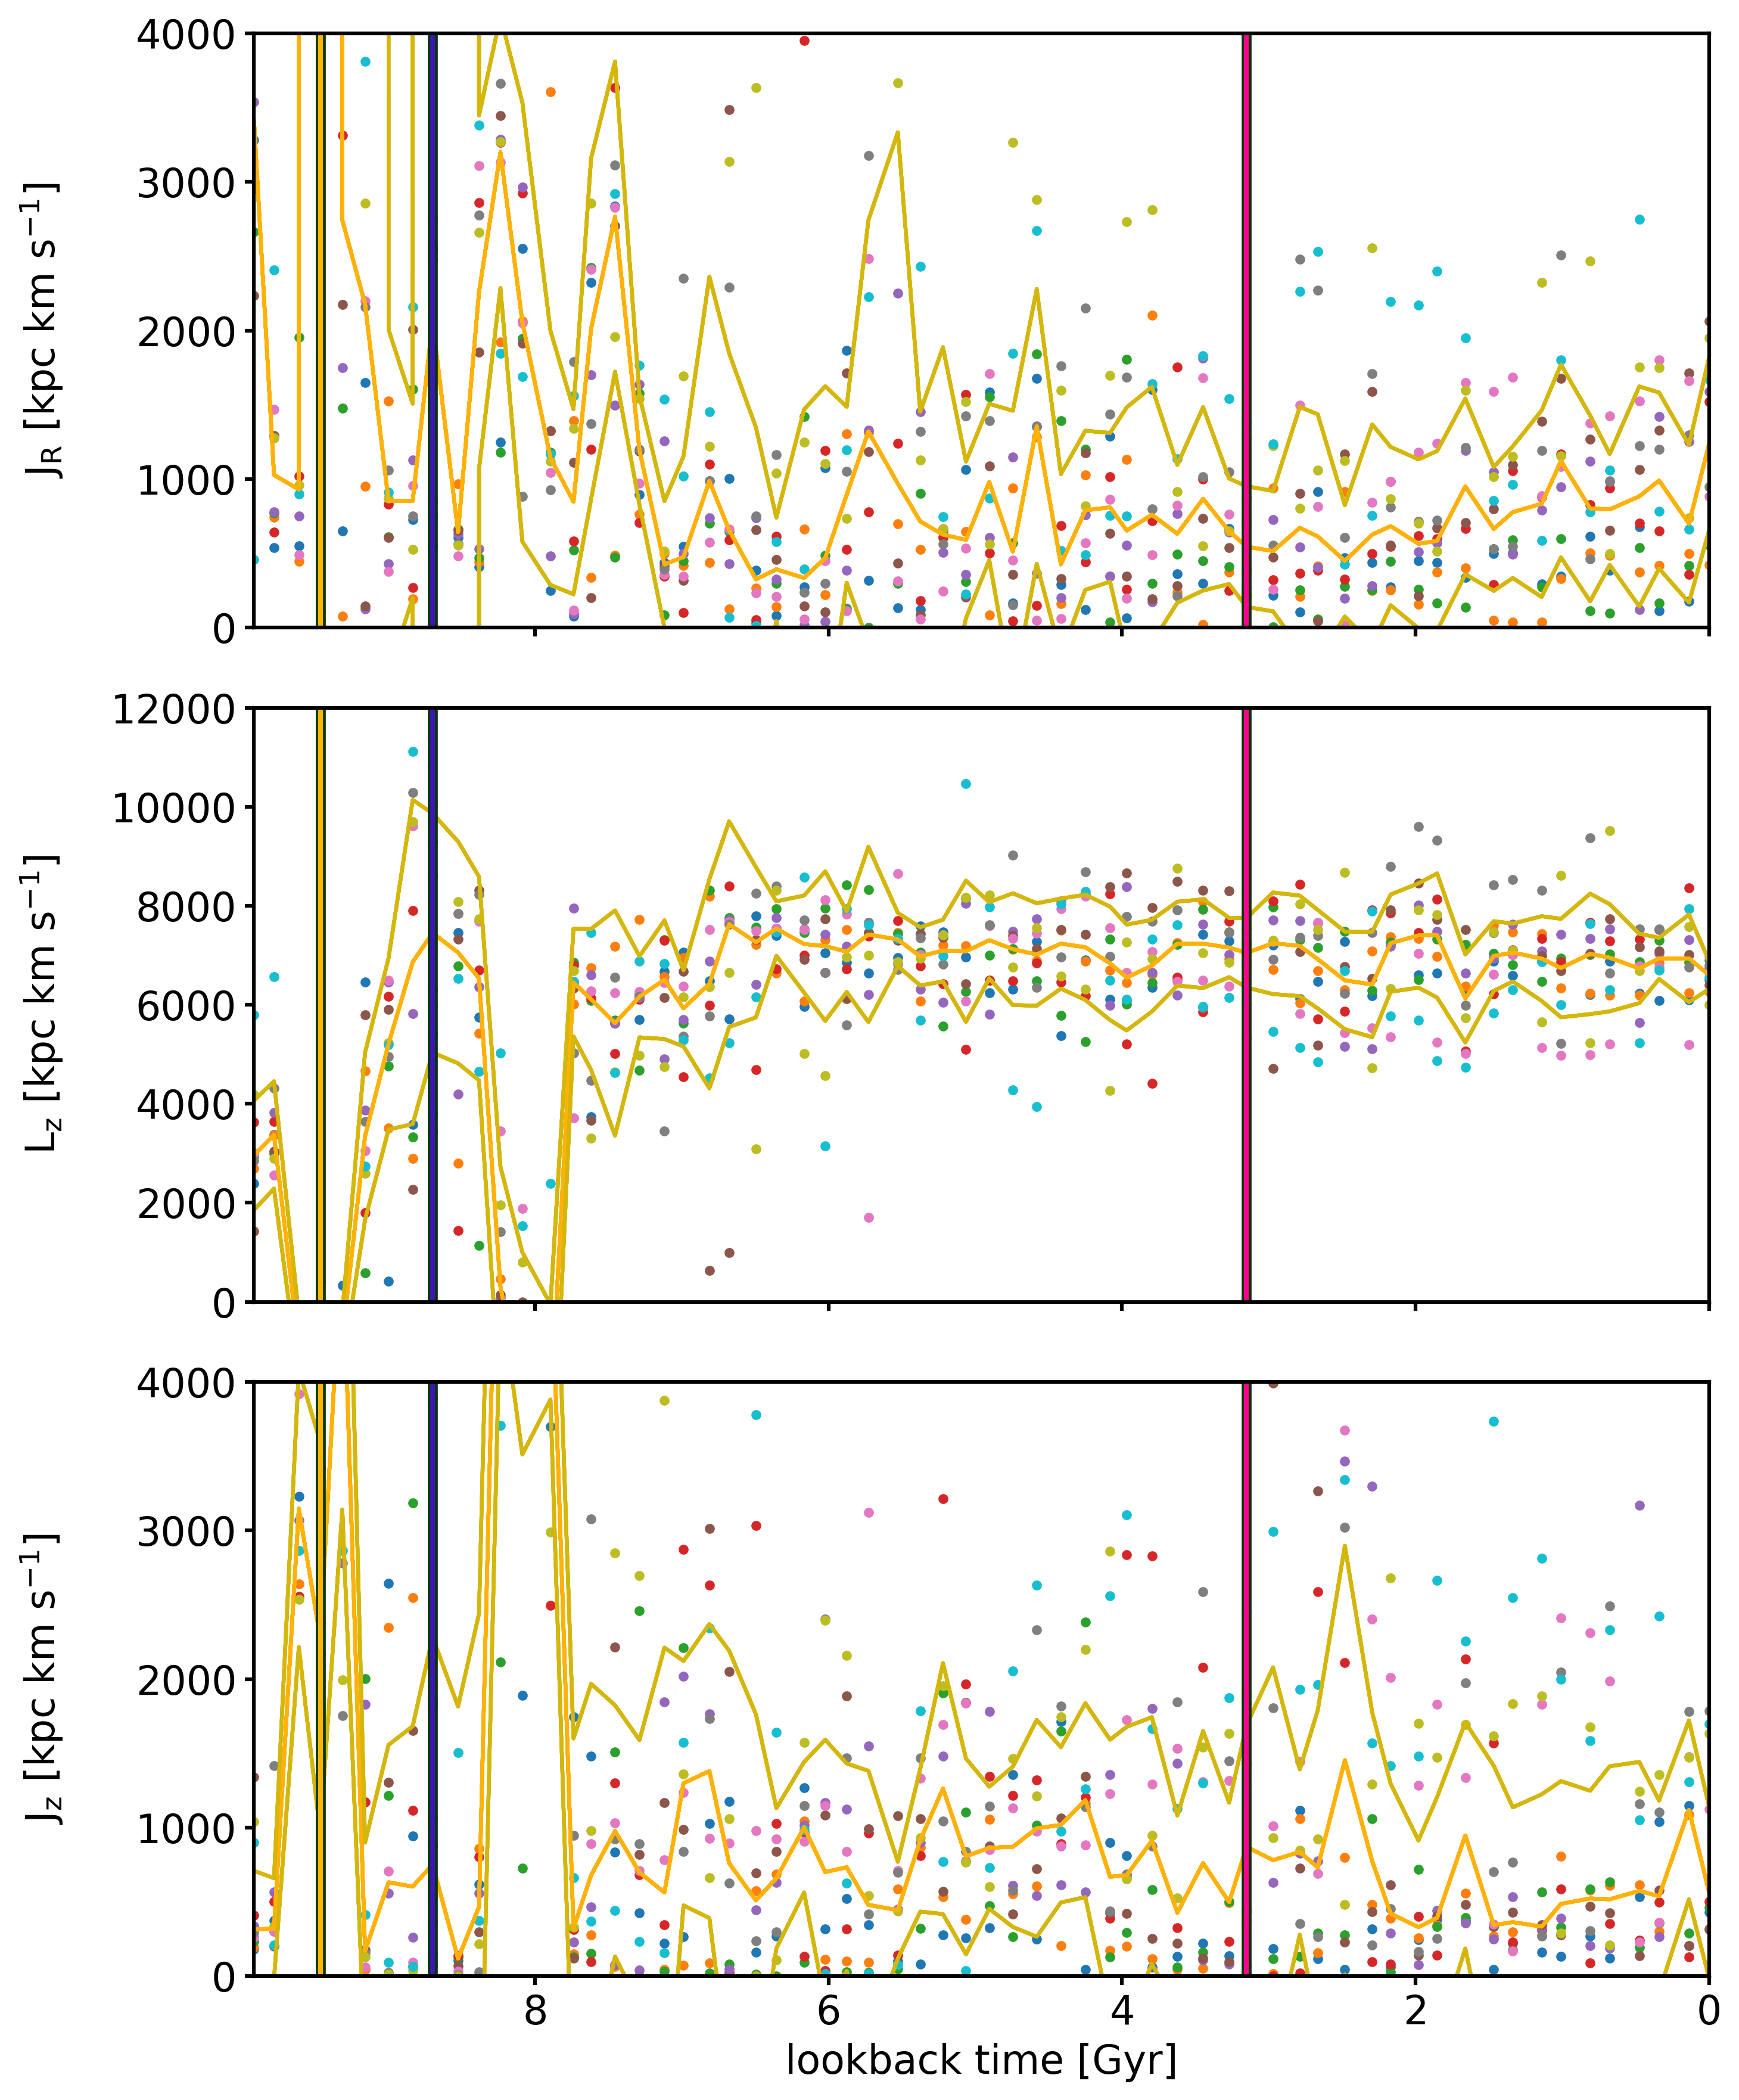
\includegraphics[width=\textwidth]{plots/Dynamics/prog4/action_time_evolution_box_hist_mean_prog4.png}
    \caption{Action time evolution of xx particles of prog4 which are on as similar orbits as possible. }\label{fig:actions_box_time_evolution_prog4}
\end{figure}
\fi

